% Generated by Sphinx.
\def\sphinxdocclass{report}
\documentclass[a4paper,12pt,oneside]{sphinxmanual}
\usepackage[utf8x]{inputenc}
\usepackage{cmap}
\usepackage[T1]{fontenc}
\usepackage[russian]{babel}
\usepackage{times}
\usepackage[Sonny]{fncychap}
\usepackage{longtable}
\usepackage{sphinx}
\usepackage{multirow}
\setkeys{Gin}{width=.80\textwidth}

\title{Blend4Web. User manual}
\date{March 21, 2014}
\release{14.03.21}
\author{Triumph LLC}
\newcommand{\sphinxlogo}{}
\renewcommand{\releasename}{Release}
\makeindex

\makeatletter
\def\PYG@reset{\let\PYG@it=\relax \let\PYG@bf=\relax%
    \let\PYG@ul=\relax \let\PYG@tc=\relax%
    \let\PYG@bc=\relax \let\PYG@ff=\relax}
\def\PYG@tok#1{\csname PYG@tok@#1\endcsname}
\def\PYG@toks#1+{\ifx\relax#1\empty\else%
    \PYG@tok{#1}\expandafter\PYG@toks\fi}
\def\PYG@do#1{\PYG@bc{\PYG@tc{\PYG@ul{%
    \PYG@it{\PYG@bf{\PYG@ff{#1}}}}}}}
\def\PYG#1#2{\PYG@reset\PYG@toks#1+\relax+\PYG@do{#2}}

\expandafter\def\csname PYG@tok@gd\endcsname{\def\PYG@tc##1{\textcolor[rgb]{0.63,0.00,0.00}{##1}}}
\expandafter\def\csname PYG@tok@gu\endcsname{\let\PYG@bf=\textbf\def\PYG@tc##1{\textcolor[rgb]{0.50,0.00,0.50}{##1}}}
\expandafter\def\csname PYG@tok@gt\endcsname{\def\PYG@tc##1{\textcolor[rgb]{0.00,0.27,0.87}{##1}}}
\expandafter\def\csname PYG@tok@gs\endcsname{\let\PYG@bf=\textbf}
\expandafter\def\csname PYG@tok@gr\endcsname{\def\PYG@tc##1{\textcolor[rgb]{1.00,0.00,0.00}{##1}}}
\expandafter\def\csname PYG@tok@cm\endcsname{\let\PYG@it=\textit\def\PYG@tc##1{\textcolor[rgb]{0.25,0.50,0.56}{##1}}}
\expandafter\def\csname PYG@tok@vg\endcsname{\def\PYG@tc##1{\textcolor[rgb]{0.73,0.38,0.84}{##1}}}
\expandafter\def\csname PYG@tok@m\endcsname{\def\PYG@tc##1{\textcolor[rgb]{0.13,0.50,0.31}{##1}}}
\expandafter\def\csname PYG@tok@mh\endcsname{\def\PYG@tc##1{\textcolor[rgb]{0.13,0.50,0.31}{##1}}}
\expandafter\def\csname PYG@tok@cs\endcsname{\def\PYG@tc##1{\textcolor[rgb]{0.25,0.50,0.56}{##1}}\def\PYG@bc##1{\setlength{\fboxsep}{0pt}\colorbox[rgb]{1.00,0.94,0.94}{\strut ##1}}}
\expandafter\def\csname PYG@tok@ge\endcsname{\let\PYG@it=\textit}
\expandafter\def\csname PYG@tok@vc\endcsname{\def\PYG@tc##1{\textcolor[rgb]{0.73,0.38,0.84}{##1}}}
\expandafter\def\csname PYG@tok@il\endcsname{\def\PYG@tc##1{\textcolor[rgb]{0.13,0.50,0.31}{##1}}}
\expandafter\def\csname PYG@tok@go\endcsname{\def\PYG@tc##1{\textcolor[rgb]{0.20,0.20,0.20}{##1}}}
\expandafter\def\csname PYG@tok@cp\endcsname{\def\PYG@tc##1{\textcolor[rgb]{0.00,0.44,0.13}{##1}}}
\expandafter\def\csname PYG@tok@gi\endcsname{\def\PYG@tc##1{\textcolor[rgb]{0.00,0.63,0.00}{##1}}}
\expandafter\def\csname PYG@tok@gh\endcsname{\let\PYG@bf=\textbf\def\PYG@tc##1{\textcolor[rgb]{0.00,0.00,0.50}{##1}}}
\expandafter\def\csname PYG@tok@ni\endcsname{\let\PYG@bf=\textbf\def\PYG@tc##1{\textcolor[rgb]{0.84,0.33,0.22}{##1}}}
\expandafter\def\csname PYG@tok@nl\endcsname{\let\PYG@bf=\textbf\def\PYG@tc##1{\textcolor[rgb]{0.00,0.13,0.44}{##1}}}
\expandafter\def\csname PYG@tok@nn\endcsname{\let\PYG@bf=\textbf\def\PYG@tc##1{\textcolor[rgb]{0.05,0.52,0.71}{##1}}}
\expandafter\def\csname PYG@tok@no\endcsname{\def\PYG@tc##1{\textcolor[rgb]{0.38,0.68,0.84}{##1}}}
\expandafter\def\csname PYG@tok@na\endcsname{\def\PYG@tc##1{\textcolor[rgb]{0.25,0.44,0.63}{##1}}}
\expandafter\def\csname PYG@tok@nb\endcsname{\def\PYG@tc##1{\textcolor[rgb]{0.00,0.44,0.13}{##1}}}
\expandafter\def\csname PYG@tok@nc\endcsname{\let\PYG@bf=\textbf\def\PYG@tc##1{\textcolor[rgb]{0.05,0.52,0.71}{##1}}}
\expandafter\def\csname PYG@tok@nd\endcsname{\let\PYG@bf=\textbf\def\PYG@tc##1{\textcolor[rgb]{0.33,0.33,0.33}{##1}}}
\expandafter\def\csname PYG@tok@ne\endcsname{\def\PYG@tc##1{\textcolor[rgb]{0.00,0.44,0.13}{##1}}}
\expandafter\def\csname PYG@tok@nf\endcsname{\def\PYG@tc##1{\textcolor[rgb]{0.02,0.16,0.49}{##1}}}
\expandafter\def\csname PYG@tok@si\endcsname{\let\PYG@it=\textit\def\PYG@tc##1{\textcolor[rgb]{0.44,0.63,0.82}{##1}}}
\expandafter\def\csname PYG@tok@s2\endcsname{\def\PYG@tc##1{\textcolor[rgb]{0.25,0.44,0.63}{##1}}}
\expandafter\def\csname PYG@tok@vi\endcsname{\def\PYG@tc##1{\textcolor[rgb]{0.73,0.38,0.84}{##1}}}
\expandafter\def\csname PYG@tok@nt\endcsname{\let\PYG@bf=\textbf\def\PYG@tc##1{\textcolor[rgb]{0.02,0.16,0.45}{##1}}}
\expandafter\def\csname PYG@tok@nv\endcsname{\def\PYG@tc##1{\textcolor[rgb]{0.73,0.38,0.84}{##1}}}
\expandafter\def\csname PYG@tok@s1\endcsname{\def\PYG@tc##1{\textcolor[rgb]{0.25,0.44,0.63}{##1}}}
\expandafter\def\csname PYG@tok@gp\endcsname{\let\PYG@bf=\textbf\def\PYG@tc##1{\textcolor[rgb]{0.78,0.36,0.04}{##1}}}
\expandafter\def\csname PYG@tok@sh\endcsname{\def\PYG@tc##1{\textcolor[rgb]{0.25,0.44,0.63}{##1}}}
\expandafter\def\csname PYG@tok@ow\endcsname{\let\PYG@bf=\textbf\def\PYG@tc##1{\textcolor[rgb]{0.00,0.44,0.13}{##1}}}
\expandafter\def\csname PYG@tok@sx\endcsname{\def\PYG@tc##1{\textcolor[rgb]{0.78,0.36,0.04}{##1}}}
\expandafter\def\csname PYG@tok@bp\endcsname{\def\PYG@tc##1{\textcolor[rgb]{0.00,0.44,0.13}{##1}}}
\expandafter\def\csname PYG@tok@c1\endcsname{\let\PYG@it=\textit\def\PYG@tc##1{\textcolor[rgb]{0.25,0.50,0.56}{##1}}}
\expandafter\def\csname PYG@tok@kc\endcsname{\let\PYG@bf=\textbf\def\PYG@tc##1{\textcolor[rgb]{0.00,0.44,0.13}{##1}}}
\expandafter\def\csname PYG@tok@c\endcsname{\let\PYG@it=\textit\def\PYG@tc##1{\textcolor[rgb]{0.25,0.50,0.56}{##1}}}
\expandafter\def\csname PYG@tok@mf\endcsname{\def\PYG@tc##1{\textcolor[rgb]{0.13,0.50,0.31}{##1}}}
\expandafter\def\csname PYG@tok@err\endcsname{\def\PYG@bc##1{\setlength{\fboxsep}{0pt}\fcolorbox[rgb]{1.00,0.00,0.00}{1,1,1}{\strut ##1}}}
\expandafter\def\csname PYG@tok@kd\endcsname{\let\PYG@bf=\textbf\def\PYG@tc##1{\textcolor[rgb]{0.00,0.44,0.13}{##1}}}
\expandafter\def\csname PYG@tok@ss\endcsname{\def\PYG@tc##1{\textcolor[rgb]{0.32,0.47,0.09}{##1}}}
\expandafter\def\csname PYG@tok@sr\endcsname{\def\PYG@tc##1{\textcolor[rgb]{0.14,0.33,0.53}{##1}}}
\expandafter\def\csname PYG@tok@mo\endcsname{\def\PYG@tc##1{\textcolor[rgb]{0.13,0.50,0.31}{##1}}}
\expandafter\def\csname PYG@tok@mi\endcsname{\def\PYG@tc##1{\textcolor[rgb]{0.13,0.50,0.31}{##1}}}
\expandafter\def\csname PYG@tok@kn\endcsname{\let\PYG@bf=\textbf\def\PYG@tc##1{\textcolor[rgb]{0.00,0.44,0.13}{##1}}}
\expandafter\def\csname PYG@tok@o\endcsname{\def\PYG@tc##1{\textcolor[rgb]{0.40,0.40,0.40}{##1}}}
\expandafter\def\csname PYG@tok@kr\endcsname{\let\PYG@bf=\textbf\def\PYG@tc##1{\textcolor[rgb]{0.00,0.44,0.13}{##1}}}
\expandafter\def\csname PYG@tok@s\endcsname{\def\PYG@tc##1{\textcolor[rgb]{0.25,0.44,0.63}{##1}}}
\expandafter\def\csname PYG@tok@kp\endcsname{\def\PYG@tc##1{\textcolor[rgb]{0.00,0.44,0.13}{##1}}}
\expandafter\def\csname PYG@tok@w\endcsname{\def\PYG@tc##1{\textcolor[rgb]{0.73,0.73,0.73}{##1}}}
\expandafter\def\csname PYG@tok@kt\endcsname{\def\PYG@tc##1{\textcolor[rgb]{0.56,0.13,0.00}{##1}}}
\expandafter\def\csname PYG@tok@sc\endcsname{\def\PYG@tc##1{\textcolor[rgb]{0.25,0.44,0.63}{##1}}}
\expandafter\def\csname PYG@tok@sb\endcsname{\def\PYG@tc##1{\textcolor[rgb]{0.25,0.44,0.63}{##1}}}
\expandafter\def\csname PYG@tok@k\endcsname{\let\PYG@bf=\textbf\def\PYG@tc##1{\textcolor[rgb]{0.00,0.44,0.13}{##1}}}
\expandafter\def\csname PYG@tok@se\endcsname{\let\PYG@bf=\textbf\def\PYG@tc##1{\textcolor[rgb]{0.25,0.44,0.63}{##1}}}
\expandafter\def\csname PYG@tok@sd\endcsname{\let\PYG@it=\textit\def\PYG@tc##1{\textcolor[rgb]{0.25,0.44,0.63}{##1}}}

\def\PYGZbs{\char`\\}
\def\PYGZus{\char`\_}
\def\PYGZob{\char`\{}
\def\PYGZcb{\char`\}}
\def\PYGZca{\char`\^}
\def\PYGZam{\char`\&}
\def\PYGZlt{\char`\<}
\def\PYGZgt{\char`\>}
\def\PYGZsh{\char`\#}
\def\PYGZpc{\char`\%}
\def\PYGZdl{\char`\$}
\def\PYGZhy{\char`\-}
\def\PYGZsq{\char`\'}
\def\PYGZdq{\char`\"}
\def\PYGZti{\char`\~}
% for compatibility with earlier versions
\def\PYGZat{@}
\def\PYGZlb{[}
\def\PYGZrb{]}
\makeatother

\begin{document}

\maketitle
\tableofcontents
\phantomsection\label{index::doc}



\chapter{Overview}
\label{about:about}\label{about::doc}\label{about:id1}
\index{{[}TODO{]}}

\section{What's Blend4Web}
\label{about:about-product}\label{about:blend4web}\label{about:index-0}
Blend4Web is {[}TODO{]}

{[}TODO{]}

{[}TODO{]}

{[}TODO{]}

\index{{[}TODO{]}}

\section{Engine}
\label{about:about-engine}\label{about:id2}\label{about:index-1}
{[}TODO{]}

{[}TODO{]}

\index{{[}TODO{]}}\index{{[}TODO{]}}

\section{Graphics Engine, Game Engine}
\label{about:about-graphics-engine}\label{about:id3}\label{about:index-2}
{[}TODO{]}
\begin{itemize}
\item {} 
{[}TODO{]}

\item {} 
{[}TODO{]}

\end{itemize}

{[}TODO{]}

\index{{[}TODO{]}}

\section{What's WebGL}
\label{about:webgl}\label{about:about-webgl}\label{about:index-3}
{[}TODO{]}

\index{{[}TODO{]}!{[}TODO{]}}

\section{WebGL support in browsers}
\label{about:index-4}\label{about:id4}\label{about:browser-webgl-support}
{[}TODO{]}


\subsection{Full support}
\label{about:id5}\begin{itemize}
\item {} 
{[}TODO{]}

\item {} 
{[}TODO{]}

\item {} 
{[}TODO{]}

\item {} 
{[}TODO{]}

\end{itemize}


\subsection{Experimental Support}
\label{about:id6}\begin{itemize}
\item {} 
{[}TODO{]}

\item {} 
{[}TODO{]}

\end{itemize}


\subsection{Mobile Platforms}
\label{about:id7}\begin{itemize}
\item {} 
{[}TODO{]}

\item {} 
{[}TODO{]}

\item {} 
{[}TODO{]}

\item {} 
{[}TODO{]}

\item {} 
{[}TODO{]}

\item {} 
{[}TODO{]}

\item {} 
{[}TODO{]}

\end{itemize}

\index{{[}TODO{]}!{[}TODO{]}}

\section{Advantages of WebGL}
\label{about:about-webgl-benefits}\label{about:index-5}\label{about:id8}\begin{itemize}
\item {} 
{[}TODO{]}

\item {} 
{[}TODO{]}

\item {} 
{[}TODO{]}

\item {} 
{[}TODO{]}

\item {} 
{[}TODO{]}

\item {} 
{[}TODO{]}

\end{itemize}

\index{{[}TODO{]}}

\section{What's Blender}
\label{about:index-6}\label{about:about-blender}\label{about:blender}
{[}TODO{]}

\index{3D modelling}

\section{3D modelling}
\label{about:about-modelling}\label{about:index-7}\label{about:d}
{[}TODO{]}

{[}TODO{]}
\begin{itemize}
\item {} 
{[}TODO{]}

\item {} 
{[}TODO{]}

\item {} 
{[}TODO{]}

\item {} 
{[}TODO{]}

\item {} 
{[}TODO{]}

\item {} 
{[}TODO{]}

\item {} 
{[}TODO{]}

\item {} 
{[}TODO{]}

\end{itemize}

{[}TODO{]}
\begin{itemize}
\item {} 
{[}TODO{]}

\item {} 
{[}TODO{]}

\item {} 
{[}TODO{]}

\item {} 
{[}TODO{]}

\item {} 
{[}TODO{]}

\item {} 
{[}TODO{]}

\end{itemize}

{[}TODO{]}

\index{{[}TODO{]}}\index{{[}TODO{]}}

\section{Browser technologies}
\label{about:id10}\label{about:index-8}\label{about:about-browser-tech}
{[}TODO{]}

{[}TODO{]}
\begin{itemize}
\item {} 
{[}TODO{]}

\item {} 
{[}TODO{]}

\item {} 
{[}TODO{]}

\item {} 
{[}TODO{]}

\item {} 
{[}TODO{]}

\item {} 
{[}TODO{]}

\item {} 
{[}TODO{]}

\item {} 
{[}TODO{]}

\item {} 
{[}TODO{]}

\end{itemize}

{[}TODO{]}
\begin{itemize}
\item {} 
{[}TODO{]}

\item {} 
{[}TODO{]}

\item {} 
{[}TODO{]}

\item {} 
{[}TODO{]}

\item {} 
{[}TODO{]}

\end{itemize}

\index{{[}TODO{]}}

\section{Interactive Graphics}
\label{about:about-interactive-graphics}\label{about:id12}\label{about:index-9}
{[}TODO{]}

{[}TODO{]}

{[}TODO{]}

\index{{[}TODO{]}}\index{{[}TODO{]}}

\section{Video Cards and Drivers}
\label{about:id13}\label{about:about-drivers-video-cards}\label{about:index-10}
{[}TODO{]}

{[}TODO{]}

{[}TODO{]}

\index{{[}TODO{]}!{[}TODO{]}}

\section{Examples of the use of 3D web technologies}
\label{about:index-11}\label{about:id14}\label{about:web3d-examples}

\subsection{Visualisation}
\label{about:id15}\begin{itemize}
\item {} 
{[}TODO{]}

\item {} 
{[}TODO{]}

\item {} 
{[}TODO{]}

\item {} 
{[}TODO{]}

\item {} 
{[}TODO{]}

\item {} 
{[}TODO{]}

\item {} 
{[}TODO{]}

\item {} 
{[}TODO{]}

\item {} 
{[}TODO{]}

\item {} 
{[}TODO{]}

\item {} 
{[}TODO{]}

\item {} 
{[}TODO{]}

\end{itemize}


\subsection{Games}
\label{about:id23}\begin{itemize}
\item {} 
{[}TODO{]}

\item {} 
{[}TODO{]}

\item {} 
{[}TODO{]}

\item {} 
{[}TODO{]}

\item {} 
{[}TODO{]}

\item {} 
{[}TODO{]}

\item {} 
{[}TODO{]}

\end{itemize}


\chapter{Функционал движка}
\label{features::doc}\label{features:features}\label{features:id1}

\section{Текстуры}
\label{features:id2}\begin{itemize}
\item {} 
текстурирование (texturing) - покрытие поверхности 3D объекта плоским изображением

\item {} 
мультитекстурирование (multitexturing) - использование для объекта нескольких текстур

\item {} 
рендеринг в текстуру (render-to-texture, RTT) для реализации вложения одной сцены в другую и постпроцессинговых эффектов

\item {} 
анизотропная фильтрация для улучшения качества обзора поверхности под косыми углами (anisotropic filtering, AF, использовано стандартное расширение WebGL)

\item {} 
поддержка текстурной компрессии (формат S3TC/DXT)

\end{itemize}


\section{Материалы}
\label{features:id3}\begin{itemize}
\item {} 
прозрачность материалов, сортировка по глубине при необходимости (z-sorting)

\item {} 
улучшенная детализация рельефных поверхностей текстурами (использован метод parallax offset mapping)

\item {} 
зависимость степени отражения от угла обзора - эффект Френеля (Fresnel)

\item {} 
динамическое отражение

\item {} 
поддержка нодовых материалов

\item {} 
гало материал для рендеринга источников света и звезд (Halo material)

\end{itemize}


\section{Освещение}
\label{features:id4}\begin{itemize}
\item {} 
освещение несколькими источниками света

\item {} 
типы источников света - прямой (directional), полусферический (hemisphere), точечный (point), конический (spot)

\item {} 
диффузное (т.е. рассеянное) освещение объектов (diffuse lighting)

\item {} 
рассеянное освещение от окружающей среды (ambient lighting)

\item {} 
зеркальное отражение света от поверхности объектов (specular lighting)

\item {} 
зеркальное отражение окружающей среды (environment mapping)

\item {} 
дополнительная детализация картами нормалей к поверхности (normal mapping)

\end{itemize}


\section{Тени}
\label{features:id5}\begin{itemize}
\item {} 
статические падающие тени (light mapping)

\item {} 
динамические падающие тени (использован метод shadow mapping)

\item {} 
собственные тени — объекты отбрасывают тени сами на себя (self-shadowing)

\item {} 
каскадные тени для больших сцен (cascaded shadow mapping, CSM)

\item {} 
мягкие тени

\end{itemize}


\section{Система частиц}
\label{features:id6}\begin{itemize}
\item {} 
система частиц (particle system) для реализации эффектов, таких как огонь, дым, брызги и т.д.

\item {} 
система частиц для расстановки (инстансинга) однородных объектов: трава, камни, листва деревьев и проч.

\end{itemize}


\section{Рендеринг наружных сцен}
\label{features:id7}\begin{itemize}
\item {} 
туман (fog)

\item {} 
купол неба/окружающего пространства (skydome)

\item {} 
эффект линз при направлении камеры на источник света (lens flares)

\item {} 
рендеринг воды

\end{itemize}


\section{Постпроцессинговые эффекты}
\label{features:id8}\begin{itemize}
\item {} 
размытие при движении (motion blur)

\item {} 
антиалиасинг - уменьшение зубчатости краев изображения в результате рендеринга в текстуру (использован метод fast approximate anti-aliasing, FXAA)

\item {} 
стерео-изображение (анаглифное, 3D очки)

\item {} 
рассеянное затенение от окружающей среды (ambient occlusion, используется метод SSAO)

\item {} 
глубина резкости для камеры (DOF)

\item {} 
сумеречные лучи (god rays)

\item {} 
эффект засветки ярких объектов (bloom)

\item {} 
огибание объектов светом (glow)

\end{itemize}


\section{Анимация}
\label{features:id9}\begin{itemize}
\item {} 
скиннинг (skinning) - деформация объекта с помощью системы костей

\item {} 
анимация перемещения, вращения, масштабирования объектов, камер и источников света

\item {} 
скелетная анимация (например, для тела персонажа)

\item {} 
вертексная анимация (например, для симуляции ткани)

\item {} 
процедурная анимация (например, изгибание растений на ветру)

\item {} 
анимация текстурных координат (например, для визуализации волн воды)

\end{itemize}


\section{Оптимизация}
\label{features:id10}\begin{itemize}
\item {} 
оптимизация отсечением по зоне видимости (frustum culling)

\item {} 
оптимизация уменьшением количества вызовов WebGL — батчинг, текстурные атласы (batching, texture atlases)

\item {} 
оптимизация уменьшением уровня детализации объектов на удалении (level of detail, LOD)

\end{itemize}


\section{Звук}
\label{features:id11}\begin{itemize}
\item {} 
звуковой движок, основанный на Web Audio API

\item {} 
поддержка различных форматов файлов с учётом различий браузеров

\item {} 
гибкое управление воспроизведением, возможность приостановки звука

\item {} 
позиционирование источников в трёхмерном пространстве

\item {} 
эффект Допплера для движущихся объектов с возможностью отключения и
компенсацией скачков в пространстве

\item {} 
управление громкостью, скоростью и задержкой воспроизведения

\item {} 
эффекты плавного перехода громкости (fade-in, fade-out, duck)

\item {} 
качественное зацикливание звуков (looping)

\item {} 
рандомизация звуковых параметров для улучшения восприятия повторяющихся звуков

\item {} 
поддержка кроссфейдерной звуковой анимации

\item {} 
динамический компрессор

\item {} 
эффективное хранение и воспроизведение длинных музыкальных композиций

\item {} 
инструменты для сведения (микширования) звуковой картины в реальном времени

\end{itemize}


\section{Физика}
\label{features:id12}\begin{itemize}
\item {} 
физика жестких тел - определение столкновений, движение, гравитация, определение высоты, опрокидывание

\item {} 
система соединителей (ограничителей) - жёсткие, гибкие, пружинящие, поворотные, скользящие итд.

\item {} 
система трассировки лучей

\item {} 
физика плавания объектов и движения в толще воды

\item {} 
физика колёсных транспортных средств

\item {} 
физика плавучих транспортных средств

\end{itemize}


\section{Событийная модель}
\label{features:id13}\begin{itemize}
\item {} 
асинхронный фреймворк для написания логики приложений

\item {} 
управление анимацией и искусственный интеллект животных и персонажей

\end{itemize}


\section{Прочее}
\label{features:id14}\begin{itemize}
\item {} 
поддержка математических кривых для моделирования удлиненных объектов (дороги, провода, река)

\item {} 
выбор пользователем объектов на 3D сцене (picking)

\item {} 
минификация (уменьшение объема) и обфускация (сокрытие) кода, необходимые для коммерческого использования движка

\item {} 
использование распределенной системы контроля версий git

\item {} 
модульная структура исходного кода

\item {} 
мощный шейдерный препроцессор с поддержкой модулей и функциональных блоков (нод)

\item {} 
удобная система для быстрого развертывания новых 3D приложений

\item {} 
тесная интеграция с системой моделирования и анимации Blender

\item {} 
опции для поддержки работы на широком спектре оборудования

\item {} 
руководство пользователя и документация для программистов

\item {} 
взаимодействие с пользователем — управление камерой, персонажем, действиями

\end{itemize}


\chapter{Экспресс-установка}
\label{first_steps:first-steps}\label{first_steps::doc}\label{first_steps:id1}

\section{Установка программы Blender}
\label{first_steps:first-steps-blender}\label{first_steps:blender}
Создание 3D сцен осуществляется в графическом пакете \href{http://ru.wikipedia.org/wiki/Blender}{Blender}, который является программным продуктом с открытым исходным кодом и распространяется бесплатно.

Должна использоваться текущая стабильная версия Blender. Загрузить Blender можно с \href{http://www.blender.org/download}{официального сайта}.

{\hfill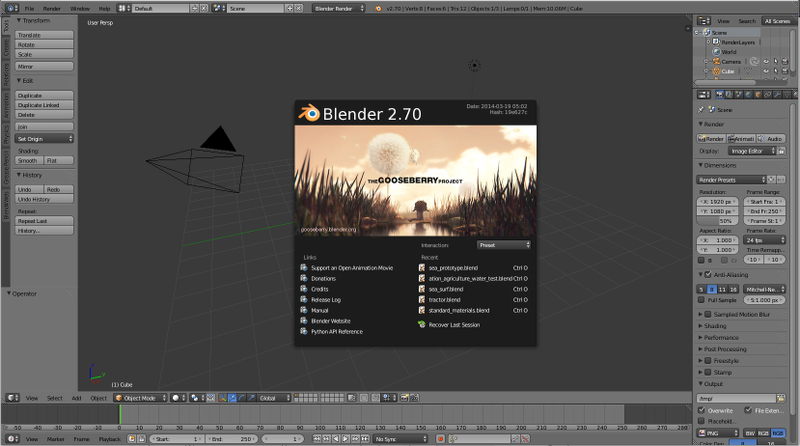
\includegraphics[width=1.000\linewidth]{blender_first_run.jpg}\hfill}

\index{экспорт!установка программы Blender}

\section{Установка аддона движка}
\label{first_steps:index-0}\label{first_steps:id4}\label{first_steps:first-step-addon}
Запустить Blender, загрузить сцену по умолчанию \code{File \textgreater{} New}.
Вызвать окно пользовательских настроек \code{File \textgreater{} User Preferences...}. Во вкладке \code{Addons} нажать \code{Install from File...} и затем выбрать zip-архив с файлами аддона. После этого необходимо отметить галочку напротив \code{Import-Export: Blend4Web}.

{\hfill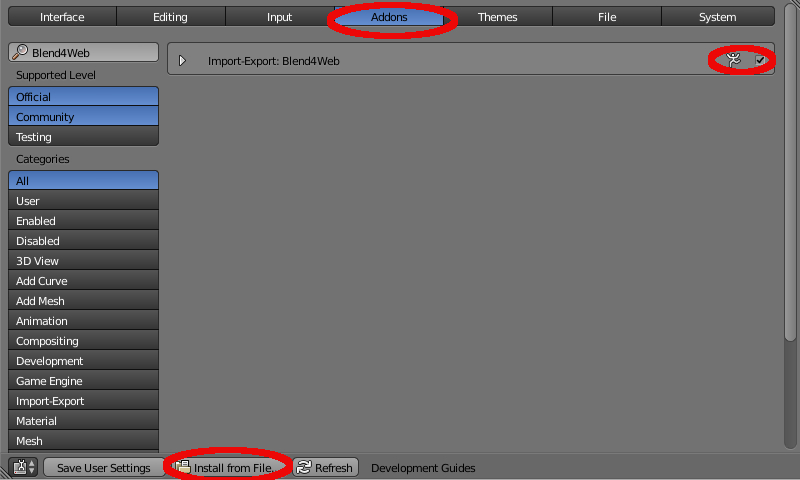
\includegraphics[width=1.000\linewidth]{user_preferences_install_b2w.jpg}\hfill}

Далее нажать \code{Save User Settings} и закрыть окно пользовательских настроек.

\index{экспорт!установка аддона}

\section{Экспорт и просмотр сцены}
\label{first_steps:first-step-export-view}\label{first_steps:id5}\label{first_steps:index-1}
Созданную сцену можно экспортировать в формате HTML. Для этого нужно выбрать опцию \code{Export \textgreater{} Blend4Web (.html)} и указать путь экспорта. Полученный HTML файл можно открыть любым браузером, поддерживающим технологию WebGL.


\strong{See also:}


{\hyperref[about:browser-webgl-support]{\emph{WebGL support in browsers}}}



\index{экспорт!просмотр сцены}

\chapter{Развёртывание среды разработки}
\label{setup:setup}\label{setup::doc}\label{setup:index-2}\label{setup:id1}
Для работы необходим дистрибутив движка, браузер (настроенный для локального
просмотра) и Blender (с установленным аддоном).


\section{Установка дистрибутива}
\label{setup:getting-started-distribution}\label{setup:id2}
Стабильные версии дистрибутива поставляются в виде архива \code{blend4web\_pro.zip}.
Для установки достаточно распаковать данный архив в любое место на диске.

Для установки дистрибутива участнику группы разработки необходимо клонировать
репозиторий (хранилище) командой:

\begin{Verbatim}[commandchars=\\\{\}]
\PYGZgt{} git clone gfxteam@192.168.89.108:blend4web.git b4w
\end{Verbatim}

В дистрибутиве находятся исходный код движка, компактная версия для приложений,
скрипты к Blender'у, исходные blend-файлы группы разработки, экспортированные
сцены, текстуры и звуковые файлы (см. подробную {\hyperref[developers:repo-file-structure]{\emph{структуру репозитория}}}).

\index{браузер!настройка}

\section{Настройка браузера}
\label{setup:index-0}\label{setup:getting-started-browser}\label{setup:id3}
Для работы движка требуется браузер с поддержкой WebGL (например, Chrome или
Firefox). Для проверки можно перейти на страницу \href{http://get.webgl.org/}{http://get.webgl.org/}. Должна
появиться надпись зеленого цвета и вращающийся куб:

{\hfill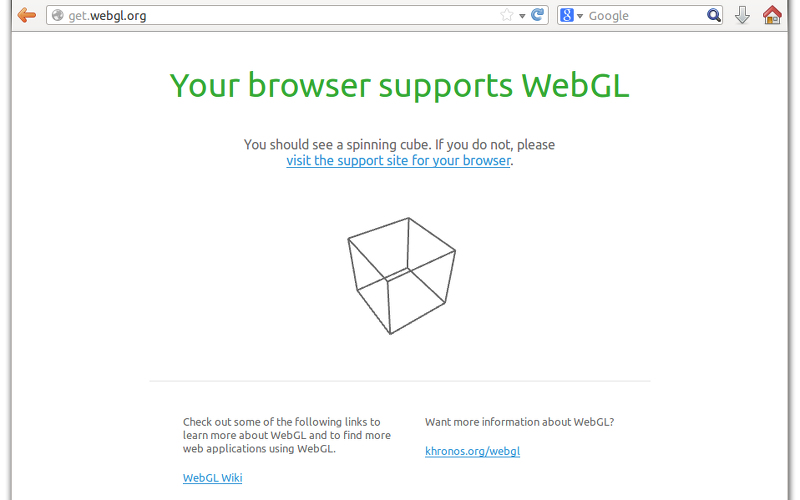
\includegraphics[width=1.000\linewidth]{browser_supports_webgl.jpg}\hfill}

\index{Blend4Web!установка}
Браузер должен быть настроен для загрузки ресурсов из локальной файловой системы. Для этого нужно указать в запускном ярлыке Chrome опцию \code{-{-}allow-file-access-from-files} (подробнее {\hyperref[problems_and_solutions:browser-for-local-loading]{\emph{о настройке}}}).

\index{просмотрщик!запуск}

\section{Запуск просмотрщика сцен}
\label{setup:id4}\label{setup:getting-started-launching-viewer}\label{setup:index-2}
Откройте файл \code{apps\_dev/viewer/viewer\_dev.html} в настроенном браузере. Должна отобразиться страница с окном рендерера и элементами интерфейса.

{\hfill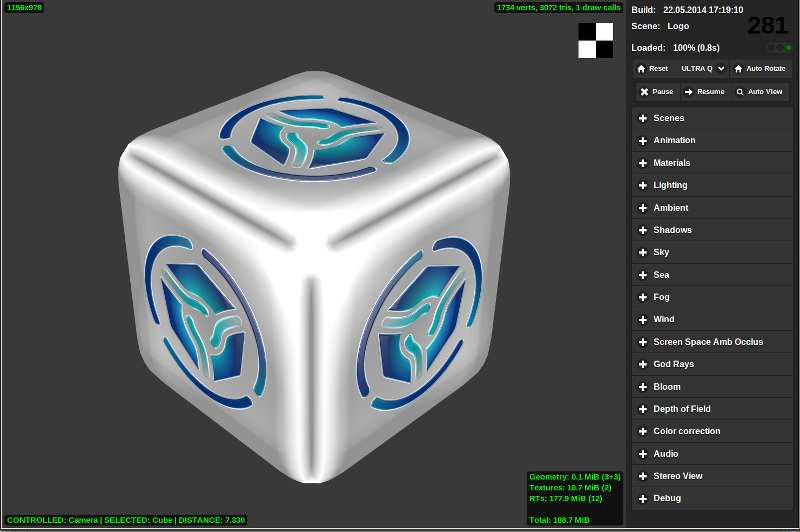
\includegraphics[width=1.000\linewidth]{default_page.jpg}\hfill}

\begin{DUlineblock}{0em}
\item[] 
\end{DUlineblock}

\begin{notice}{note}{Note:}
Если страница не отображается корректно, или появляются сообщения об ошибках, необходимо предпринять действия, описанные в разделе {\hyperref[problems_and_solutions:renderer-not-working]{\emph{Проблемы при запуске рендерера}}}.
\end{notice}

\index{Blender!установка}

\section{Установка аддона движка}
\label{setup:getting-started-addon}\label{setup:id5}\label{setup:index-3}
Запустить Blender, загрузить сцену по умолчанию \code{File \textgreater{} New} (горячие клавиши \code{Ctrl-N}).
Вызвать окно пользовательских настроек \code{File \textgreater{} User Preferences...} (горячие клавиши \code{Ctrl-Alt-U}). Во вкладке  \code{File} в поле  \code{Scripts} выбрать путь к директории \code{blender\_scripts}.

{\hfill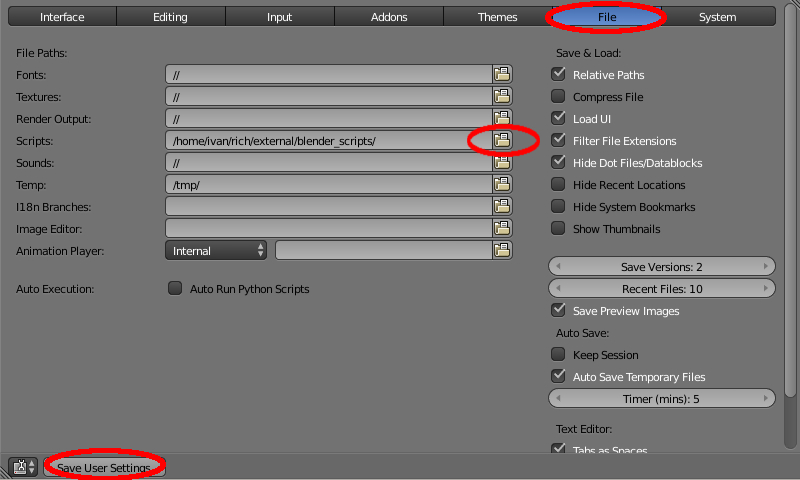
\includegraphics[width=1.000\linewidth]{user_preferences_scripts_path.jpg}\hfill}

Нажать \code{Save User Settings} и перезапустить Blender.

\emph{Примечание:}

Вместо этого можно скопировать директорию со скриптами \code{blender\_scripts/addons/blend4web} в уже используемую пользовательскую директорию для скриптов или даже в установочную директорию, например:

\code{C:\textbackslash{}Program Files\textbackslash{}Blender Foundation\textbackslash{}Blender\textbackslash{}2.69\textbackslash{}scripts\textbackslash{}addons\textbackslash{}blend4web}.

Повторно загрузить сцену по умолчанию, вызвать окно пользовательских настроек, перейти на вкладку \code{Addons} и выбрать категорию \code{Import-Export}. Отметить галочку напротив \code{Import-Export: Blend4Web}.
Также можно указать, где находятся исходные файлы для экспорта сцены в формате html (поле \code{Path to b4w source}). Стандартный путь для них (относительно корня движка): \code{external/deploy/apps/embed}.

{\hfill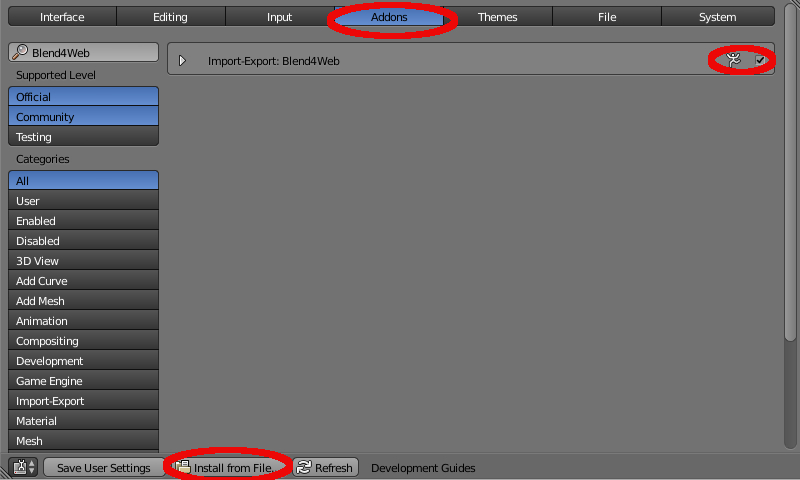
\includegraphics[width=1.000\linewidth]{user_preferences_enable_addon.jpg}\hfill}

Нажать \code{Save User Settings}. Перезапуск Blender не требуется.

\emph{Для проверки:}

В меню \code{File \textgreater{} Export} должны появиться опции \code{Blend4Web (.json)} и \code{Blend4Web (.html)}. Кроме того должны появиться операторы при выполнении поиска по ``B4W'' (горячая клавиша \code{ПРОБЕЛ}).


\chapter{Рабочий процесс}
\label{working_process_stages::doc}\label{working_process_stages:working-process-stages}\label{working_process_stages:id1}
Создание любого продукта является творческим процессом, в котором могут
участвовать множество людей, с различными навыками и опытом. Однако вне
зависимости от его сложности и конечного результата, всегда можно выделить
стадию производства, на которой создаётся основной объём ресурсов (ассетов) и
исходного кода.

При использовании Blend4Web, производственный процесс можно представить
следующим образом:
\begin{enumerate}
\item {} 
Подготовка трёхмерной сцены в программе Blender.

\item {} 
Экспорт ресурсов в формате, пригодном для использования движком.

\item {} 
Запуск, настройка и отладка сцены в программе-просмоторщике.

\item {} 
Создание целевого приложения.

\end{enumerate}


\section{Подготовка сцен}
\label{working_process_stages:id2}
Помимо обычных операций по моделированию, текстурированию, анимации и т.д.
должна быть осуществлена подготовка сцены для работы в движке.

Общие рекомендации:
\begin{enumerate}
\item {} 
Blend-файлы должны находиться в директории \code{external/blender/имя\_проекта}.

\item {} 
Файлы текстур должны быть внешними и находиться в директории \code{external/deploy/assets/имя\_проекта}.

\item {} 
Вспомогательные файлы, не предназначенные для загрузки в движок (например, референсы), должны находиться в директории \code{external/blender/имя\_проекта}.

\item {} 
Файл, из которого будет осуществляться экспорт, должен содержать только необходимые в разрабатываемом приложении модели.

\item {} 
Объект, меш, материал, текстура, арматура должны иметь отличающие названия (на англ. языке). Они не должны называться ``Cube.001'', ``Material'', ``Armature''.

\item {} 
Допускается добавление по ссылке (linking) компонентов из других файлов (библиотек).

\end{enumerate}

\index{экспорт}

\section{Экспорт сцен}
\label{working_process_stages:index-0}\label{working_process_stages:id3}
Для загрузки сцен, созданных с помощью пакета Blender, в движок, необходимо перевести их в формат, пригодный для чтения браузером. На данный момент используются текстовые файлы с расширением \code{.json}, в которые сохраняются экспортируемые структуры данных в формате JSON (JavaScript Object Notation).

Экспорт производится выбором в меню \code{File \textgreater{} Export} опции \code{Blend4Web (.json)}. Быстрый доступ - поиск по \code{b4w export} (горячая клавиша \code{ПРОБЕЛ}).

Экспортные файлы должны находиться в директории \code{external/deploy/assets/имя\_проекта}.

Необходимо использовать относительные пути для изображений (как правило, это происходит по умолчанию). В случаях, когда это не так, необходимо выполнить команду \code{File \textgreater{} External Data \textgreater{} Make All Paths Relative} (т.е. сделать все пути относительными). Использование абсолютных путей вместо относительных может приводить к ошибкам при попытках загрузки \code{.blend} и \code{.json} файлов на других компьютерах.

В момент экспорта происходит проверка сцены на предмет использования не поддерживаемых движком возможностей Blender'a. В таких случаях генерируется сообщение об ошибке:

{\hfill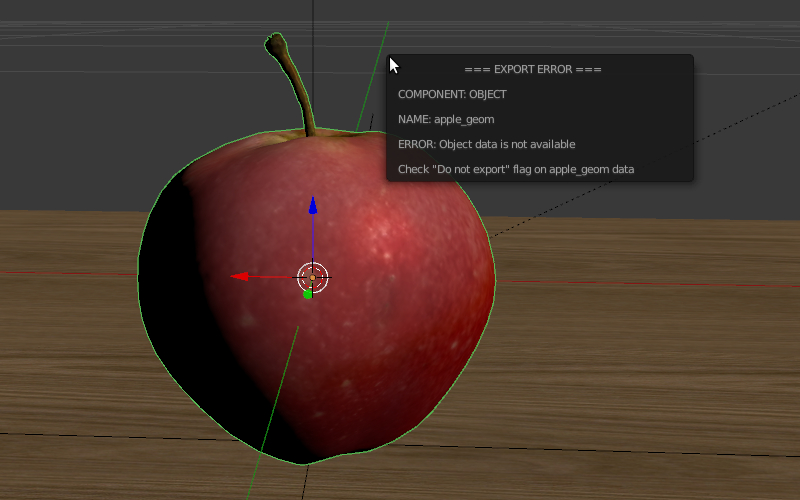
\includegraphics[width=1.000\linewidth]{error_message.jpg}\hfill}

\begin{DUlineblock}{0em}
\item[] 
\end{DUlineblock}

Перечень возможных ошибок экспорта перечислен в {\hyperref[export_errors:export-errors]{\emph{соответствующем разделе}}}.


\subsection{Опции экспорта}
\label{working_process_stages:id4}\begin{description}
\item[{\emph{Autosave main file}}] \leavevmode
Автосохранение файла, из которого осуществляется экспорт. \textbf{Включено по умолчанию}. Осуществляется непосредственно после экспорта с целью поддержки соответствия между текущим содержимым blend-файла и экспортного файла. Кроме того, для удобства в blend-файле сохраняется относительный путь к экспортному файлу.

\item[{\emph{Filepath}}] \leavevmode
Путь для экспортного файла. Используется в режиме экспорта из командой строки. В оконном режиме не используется.

\end{description}

\index{просмотрщик!добавление сцен}

\section{Отображение сцен в просмоторщике}
\label{working_process_stages:id5}\label{working_process_stages:index-1}
Для того, чтобы сцена появилась в списке сцен просмотрщика, нужно добавить запись в текстовой файл \code{external/deploy/assets/assets.js}.

Для добавления новой сцены нужно знать категорию, в которой она должна отображаться. Категория обычно соответствует названию проекта и имени директории, где хранятся соответствующие файлы.


\subsection{Пример}
\label{working_process_stages:id6}
Ниже приведена примерная часть файла \code{assets.js}, в которой находятся два проекта ``Capri'' и ``Fridge'' с соответствующими сценами в каждом проекте:

\begin{Verbatim}[commandchars=\\\{\}]
\PYG{p}{\PYGZob{}}
    \PYG{n}{name}\PYG{p}{:} \PYG{l+s}{\PYGZdq{}}\PYG{l+s}{Capri}\PYG{l+s}{\PYGZdq{}}\PYG{p}{,}
    \PYG{n}{items}\PYG{p}{:} \PYG{p}{[}
        \PYG{p}{\PYGZob{}}
            \PYG{n}{name}\PYG{p}{:} \PYG{l+s}{\PYGZdq{}}\PYG{l+s}{Baken}\PYG{l+s}{\PYGZdq{}}\PYG{p}{,}
            \PYG{n}{load\PYGZus{}file} \PYG{p}{:} \PYG{l+s}{\PYGZdq{}}\PYG{l+s}{capri/props/baken/baken.json}\PYG{l+s}{\PYGZdq{}}
        \PYG{p}{\PYGZcb{}}\PYG{p}{,}
        \PYG{p}{\PYGZob{}}
            \PYG{n}{name}\PYG{p}{:} \PYG{l+s}{\PYGZdq{}}\PYG{l+s}{Terrain}\PYG{l+s}{\PYGZdq{}}\PYG{p}{,}
            \PYG{n}{load\PYGZus{}file} \PYG{p}{:} \PYG{l+s}{\PYGZdq{}}\PYG{l+s}{capri/landscape/terrain/terrain.json}\PYG{l+s}{\PYGZdq{}}
        \PYG{p}{\PYGZcb{}}
    \PYG{p}{]}
\PYG{p}{\PYGZcb{}}\PYG{p}{,}
\PYG{p}{\PYGZob{}}
    \PYG{n}{name}\PYG{p}{:} \PYG{l+s}{\PYGZdq{}}\PYG{l+s}{Fridge}\PYG{l+s}{\PYGZdq{}}\PYG{p}{,}
    \PYG{n}{items}\PYG{p}{:} \PYG{p}{[}
        \PYG{p}{\PYGZob{}}
            \PYG{n}{name}\PYG{p}{:} \PYG{l+s}{\PYGZdq{}}\PYG{l+s}{Apple}\PYG{l+s}{\PYGZdq{}}\PYG{p}{,}
            \PYG{n}{load\PYGZus{}file} \PYG{p}{:} \PYG{l+s}{\PYGZdq{}}\PYG{l+s}{fridge/fruits/apple/apple.json}\PYG{l+s}{\PYGZdq{}}
        \PYG{p}{\PYGZcb{}}\PYG{p}{,}
        \PYG{p}{\PYGZob{}}
            \PYG{n}{name}\PYG{p}{:} \PYG{l+s}{\PYGZdq{}}\PYG{l+s}{Mango}\PYG{l+s}{\PYGZdq{}}\PYG{p}{,}
            \PYG{n}{load\PYGZus{}file} \PYG{p}{:} \PYG{l+s}{\PYGZdq{}}\PYG{l+s}{fridge/fruits/mango/mango.json}\PYG{l+s}{\PYGZdq{}}
        \PYG{p}{\PYGZcb{}}
    \PYG{p}{]}
\PYG{p}{\PYGZcb{}}
\end{Verbatim}

Добавление можно осуществить копированием и вставкой описания похожей сцены в нужной категории и последующим редактированием ее названия и пути к экспортному файлу.

В случае успешного добавления сцена должна появиться в списке сцен просмотрщика в нужной категории.

{\hfill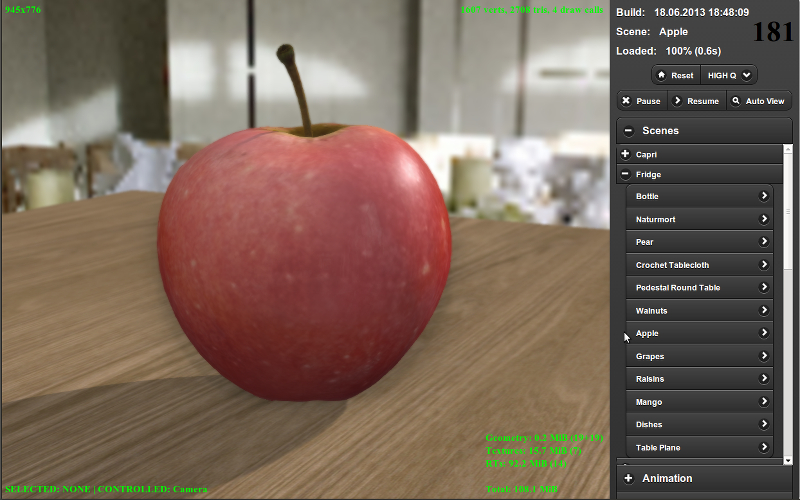
\includegraphics[width=1.000\linewidth]{viewer_apple_scene.jpg}\hfill}


\section{Создание приложения}
\label{working_process_stages:id7}
На этой стадии создаётся общий вид приложения и пишется исходный код. Документация для разработчиков приложений приведена в {\hyperref[developers:developers]{\emph{соответствующем разделе}}}.

\index{просмотрщик}

\chapter{Просмотрщик сцен}
\label{viewer:viewer}\label{viewer:index-0}\label{viewer::doc}\label{viewer:id1}
{\hyperref[setup:getting-started-launching-viewer]{\emph{Запуск просмотрщика сцен}}}.


\section{Навигация}
\label{viewer:id2}
Вращение камеры осуществляется клавишами \code{W}, \code{A}, \code{S}, \code{D}, \code{R}, \code{F}: вперед, влево, назад, вправо, вверх, вниз. Также поддерживаются стрелки и клавиши \code{numpad}. В зависимости от настроек камеры (режим движения Target) возможно целеуказание на выделенный объект, для чего используется клавиша \code{Z} или \code{.(точка)}.


\section{Боковая панель}
\label{viewer:id3}
Боковая панель содержит в себе три области: информационное табло, базовые кнопки
управления и список выпадающих панелей, содержащий дополнительные элементы управления, разделённые по функциональному признаку.

{\hfill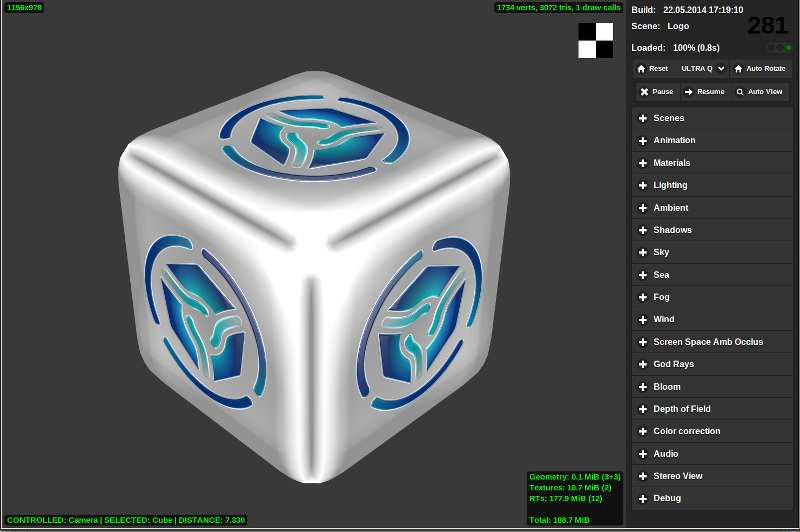
\includegraphics[width=1.000\linewidth]{default_page.jpg}\hfill}

\begin{DUlineblock}{0em}
\item[] 
\end{DUlineblock}

Список элементов управления сверху вниз:
\begin{description}
\item[{\textbf{Build}}] \leavevmode
Дата и время сборки движка.

\item[{\textbf{Scene}}] \leavevmode
Название загруженной сцены, взятое из файла \code{assets.js}. При наведении курсора мыши всплывает путь к файлу.

\item[{\textbf{Loaded}}] \leavevmode
Процент и время загрузки.

\item[{\textbf{Reset}}] \leavevmode
Кнопка сброса настроек и возврата к базовой сцене.

\item[{\textbf{HIGH Q - LOW Q - COMPAT}}] \leavevmode
Выпадающее меню выбора профиля работы движка: высокое качество (максимальный набор функций), среднее качество (отключен ряд функций, размер текстур уменьшен вдвое), режим совместимости (минимум функций).

\item[{\textbf{Pause}}] \leavevmode
Приостановка рендеринга.

\item[{\textbf{Resume}}] \leavevmode
Возобновление рендеринга.

\item[{\textbf{Auto View}}] \leavevmode
Активация режима автоматического переключения сцен.

\item[{\textbf{Scenes}}] \leavevmode
Список категорий и сцен из файла \code{assets.js}.

\item[{\textbf{Animation}}] \leavevmode
Управление анимацией. При просмотре анимированных моделей можно переключать анимацию с помощью выпадающего меню, останавливать и возобновлять анимацию, выставлять кадр, отключать циклическую анимацию.

\item[{\textbf{Sound}}] \leavevmode
Управление звуком. Содержит упрощённый микшер для управления всеми источниками звука.

\item[{\textbf{Materials}}] \leavevmode
Настройка свойств материалов.

\item[{\textbf{Ambient}}] \leavevmode
Управление освещением от окружающей среды.

\item[{\textbf{Lighting}}] \leavevmode
Управление прямым освещением.

\item[{\textbf{Sky}}] \leavevmode
Настройка параметров динамического неба.

\item[{\textbf{Shadows}}] \leavevmode
Настройка теней.

\item[{\textbf{Screen Space Amb Occlus}}] \leavevmode
Настройка параметров взаимного затенения.

\item[{\textbf{Fog}}] \leavevmode
Настройка тумана.

\item[{\textbf{Depth of Field}}] \leavevmode
Настройка глубины резкости.

\item[{\textbf{God Rays}}] \leavevmode
Настройка сумеречных лучей.

\item[{\textbf{Color correction}}] \leavevmode
Цветовая коррекция.

\item[{\textbf{Anti-aliasing}}] \leavevmode
Настройка параметров сглаживания.

\item[{\textbf{Stereo View}}] \leavevmode
Управление режимом стерео-изображения.

\item[{\textbf{Wind}}] \leavevmode
Настройка ветра.

\end{description}


\section{Индикаторы}
\label{viewer:id4}\begin{description}
\item[{\textbf{Счетчик количества кадров в секунду}}] \leavevmode
Находится в правом верхнем углу. Выводит усредненные и округленные значения для процесса рендеринга и симуляции физики соответственно.

\item[{\textbf{Размер области рендеринга}}] \leavevmode
Находится в левом верхнем углу. Выводит размер области рендеринга в пикселах.

\item[{\textbf{Выбранный объект и контролируемый объект}}] \leavevmode
Находится в левом нижнем углу. Выводит название выбранного объекта и контролируемого объекта. Выбор объекта осуществляется мышью. Для получения прямого контроля над объектом (обычно в целях проверки физики) нужно нажать \code{Q} и выбрать объект. Движение объекта осуществляется клавишами \code{W}, \code{A}, \code{S}, \code{D}. Для выхода из режима контроля нужно нажать \code{Q} и ``кликнуть'' на пустом пространстве.

\item[{\textbf{Индикатор сложности сцены}}] \leavevmode
Находится в правом верхнем углу области рендеринга. Выводит количество вертексов, треугольников и WebGL вызовов.

\item[{\textbf{Индикатор памяти}}] \leavevmode
Находится в правом нижнем углу области рендеринга. Выводит количество памяти, занимаемой геометрией, текстурами, буферами с результатами рендеринга (render targets), а также суммарное количество занимаемой памяти.

\end{description}

{\hfill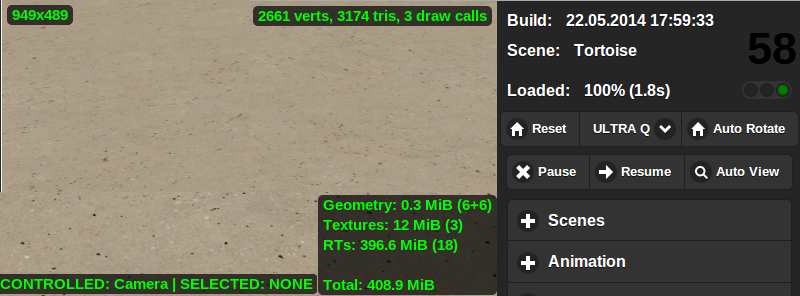
\includegraphics[width=1.000\linewidth]{indicators.jpg}\hfill}

\index{экспорт!ошибки}

\chapter{Ошибки экспорта}
\label{export_errors:index-0}\label{export_errors:export-errors}\label{export_errors::doc}\label{export_errors:id1}
При возникновении ошибок во время экспорта появляется диалоговое окно \code{BLEND2WEB EXPORT ERROR} с описанием проблемы:
\begin{quote}

\code{COMPONENT} - тип компонента (объект, меш, материал, текстура и т.д.), при экспорте которого произошла ошибка.

\code{NAME} - имя компонента.

\code{ERROR} - краткое описание возникшей проблемы на англ. языке.
\end{quote}

{\hfill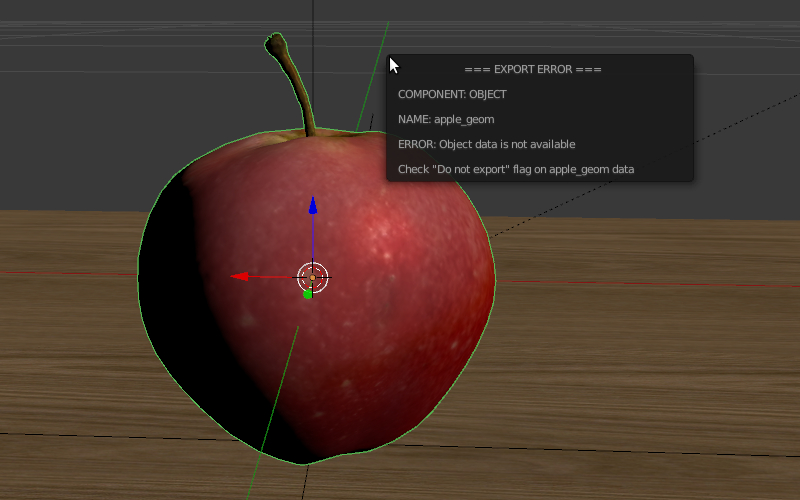
\includegraphics[width=1.000\linewidth]{error_message.jpg}\hfill}

\begin{DUlineblock}{0em}
\item[] 
\end{DUlineblock}

\begin{tabulary}{\linewidth}{|L|L|}
\hline
\textsf{\relax 
Сообщение об ошибке
} & \textsf{\relax 
Причина
}\\
\hline
Dupli group error; Objects from
dupli group GROUP\_NAME on object
OBJECT\_NAME don't export
 & 
Ни один из объектов группы GROUP\_NAME,
выбранной для дублирования на объекте
OBJECT\_NAME, не экспортируется. Требуется
разрешить экспорт хотя бы одного из
объектов группы, либо убрать дублирование
группой.
\\

Incompatible meshes; Check
MESH\_NAME1 and MESH\_NAME2 UV Maps/
Vertex colors
 & 
Имеется два меша с одинаковом материалом.
Такие меши автоматически сливаются в один
движком в целях оптимизации, и поэтому
должны иметь одинаковое число текстурных
развёрток (\code{UV Maps}) и слоёв
вертексных цветов (\code{Vertex Colors}).
\\

Incompatible objects with
shared mesh; Object OBJECT\_NAME
has vertex groups and shared mesh
 & 
Несовместимые объекты с общим мешем.
Не допускается экспорт объекта с общим
мешем и вертексными группами. Исключения:
экспорт возможен, если
на объекте включены опции
\code{Apply modifiers},
\code{Export vertex animation},
\code{Export edited normals}
(т.к. в этом случае при экспорте
происходит полное копирование мешей).
\\

Incomplete mesh; Dynamic grass
vertex colors required
by material settings
 & 
Неполный меш: специальный материал для
ландшафта использует опции
\code{Dynamic grass size} и/или
\code{Dynamic grass color}, но у меша нет
слоев вертексного цвета с такими именами.
\\

Incomplete mesh; Material slot is
empty
 & 
Неполный меш: пустой слот материала.
\\

Incomplete mesh; No UV in mesh
with UV-textured material
 & 
Неполный меш: в материале меша
используются текстуры с типом координат
\code{UV}, но у меша нет текстурной
развертки.
\\

Incomplete mesh; Vertex colors
required by material settings
 & 
Неполный меш: материал меша имеет
включенную опцию вертексного цвета
(\code{Vertex Color Paint}), но у меша нет
слоя вертексного цвета.
\\

Incorrect mesh; Wrong group indices
 & 
Меш содержит вершины, привязанные к
несуществующей группе.
\\

Incorrect vertex animation; Mesh
hasn't any vertex animation
 & 
Включен экспорт вертексной анимации для
меша, но ни одной анимации не имеется.
\\

Incorrect vertex animation; Unbaked
vertex animation ``ANIM\_NAME''
 & 
Включен экспорт вертексной анимации для
меша, но анимация ANIM\_NAME не содержит
ни одного кадра.
\\

Material has normalmap but doesn't
have material node
 & 
Нодовый материал использует
\code{Normal Mapping}, но не имеет ноды
\code{Material}.
\\
\hline\end{tabulary}


\begin{tabulary}{\linewidth}{|L|L|}
\hline

Mesh has UV map but lacks any
exported material
 & 
Меш имеет текстурную развертку, но не
имеет материала, который бы
экспортировался.
\\

Mesh has vertex color layer but
lacks any exported material
 & 
Меш имеет слой вертексного цвета, но не
имеет материала, который бы
экспортировался.
\\

Missing active camera
 & 
На сцене отсутствует активная камера
(свойство \code{Camera} на вкладке
\code{Scene}).
\\

Missing lamp
 & 
На сцене должен быть хотя бы один
источник света.
\\

Missing world
 & 
На сцене должен быть хотя бы один мир.
\\

No image
 & 
У текстуры отсутствует изображение.
\\

No such file or directory
 & 
Данная директория не существует.
\\

No texture in texture slot
 & 
В текстурном слоте материала отсутствует
текстура.
\\

Node material is invalid; Check
sockets compatibility: FROM\_NODE to
TO\_NODE
 & 
Ошибка нодового материала. Типы входа и
выхода связи между нодами \code{FROM\_NODE} и
\code{TO\_NODE} не соответствуют друг другу.
\\

Object constraint has no target
 & 
Для ограничителя объекта
(вкладка \code{Object Constraints})
не установлено свойство
\code{Target Object}.
\\

Object data is not available;
Check ``Do not export'' flag
on OBJECT\_NAME data
 & 
Не доступны данные для объекта.
Ошибка, в частности, проявляется,
когда у экспортируемого объекта
во вкладке \code{Object Data} установлено
свойство \code{Do not export}.
\\

Object-parent relation is not
supported; Clear parent inverse
transform
 & 
При использовании отношения
родитель-потомок для объекта-потомка
требуется сбросить перемещение
командой
\code{Object \textgreater{} Parent \textgreater{} Clear Parent Inverse}
(Alt-P).
\\

Only 2 UV textures are allowed for
mesh; Mesh has N UVs
 & 
Движком поддерживаются только 2 UV
текстуры на каждый меш. Меш содержит UV
текстуры в количестве N.
\\

Particle system error; Dupli group
isn't specified
 & 
Ошибка системы частиц. Не выбрана группа,
используемая в качестве частицы.
\\

Particle system error; Dupli object
isn't specified
 & 
Ошибка системы частиц. Не выбран объект,
используемый в качестве частицы.
\\

Particle system error; Dupli object
OBJECT\_NAME doesn't export
 & 
Ошибка системы частиц. Объект
OBJECT\_NAME, выбранный в качестве
частицы, не экспортируется (на нем
выбрана опция \code{Do not export}).
\\
\hline\end{tabulary}


\begin{tabulary}{\linewidth}{|L|L|}
\hline

Particle system error; No one valid
object exports from dupli group
GROUP\_NAME
 & 
Ошибка системы частиц. Ни один подходящий
объект из группы GROUP\_NAME, выбранной в
качестве частицы, не экспортируется.
Либо на таких объектах выбрана опция
\code{Do not export}, либо объекты имеют
неподходящий тип.
Поддерживаемые типы: \code{MESH}.
\\

Particle system error; Vertex color
``NAME''(from\_name) missing in object
OBJECT\_NAME
 & 
Ошибка системы частиц. Вертексный цвет
NAME указанный в поле \code{from},
отсутствует в эмиттере OBJECT\_NAME.
\\

Particle system error; Vertex color
``NAME''(to\_name) missing in object
``OBJECT\_NAME'' in dupli group
``GROUP\_NAME''
 & 
Ошибка системы частиц. Вертексный цвет
NAME указанный в поле \code{to}, не
присутствует в объекте OBJECT\_NAME группы
GROUP\_NAME, выбранной в качестве частицы.
\\

Particle system error; Vertex color
``NAME''(to\_name) missing in object
OBJECT\_NAME
 & 
Ошибка системы частиц. Вертексный цвет
NAME указанный в поле \code{to}, отсутствует
в объекте OBJECT\_NAME, выбранном в
качестве частицы.
\\

Particle system error; Wrong dupli
object type TYPE\_NAME
 & 
Ошибка системы частиц. В качестве частицы
выбран объект неподходящего типа.
Поддерживаемые типы: \code{MESH}.
\\

Permission denied
 & 
Нет прав доступа к текушей директории.
\\

Wind bending: vertex colors weren't
properly assigned
 & 
Настройки процедурной анимации деревьев;
должны быть указаны названия слоев
вертексных цветов, либо только главного:
\code{Main stiffness (A)},
либо всех сразу:
\code{Main stiffness (A)},
\code{Leaves stiffness (R)},
\code{Leaves phase (G)},
\code{Overall stiffness (B)},
либо ни одного из них.
\\

Wind bending: not all
vertex colors exist
 & 
Настройки процедурной анимации деревьев:
должны существовать все указанные
слои вертексных цветов.
\\

Wrong edited normals count; It
doesn't match with mesh vertices
count
 & 
Число редактируемых нормалей не
совпадает с числом вершин меша.
Требуется сделать \code{Clean Up} либо
\code{Save} в панели
\code{B4W Vertex Normals Editor}.
\\

Wrong overrided bounding box; Check
mesh's bounding box values
 & 
Указаны неверные размеры при
переопределении \code{BoundingBox} для меша:
минимальное значение больше максимального
для хотя бы одного из измерений.
\\

Wrong texture coordinates type
 & 
Для текстур с изображением (image)
поддерживаются следующие типы координат:
\code{UV}, \code{Normal}.
\\

Wrong vertex animation vertices
count; It doesn't match with mesh
vertices count for ``ANIM\_NAME''
 & 
Включен экспорт вертексной анимации, но
число вершин покадрово в анимации
ANIM\_NAME не совпадает с числом вершин
меша.
\\
\hline\end{tabulary}



\chapter{Объекты}
\label{objects:objects}\label{objects::doc}\label{objects:id1}
Объекты служат целям размещения компонентов различного типа (мешей, камер, ламп и т.д.) в пространстве 3D сцены.


\section{Типы}
\label{objects:id2}
Движком поддерживаются объекты следующих типов:
\begin{itemize}
\item {} 
меш (mesh)

\item {} 
камера (camera)

\item {} 
лампа (lamp)

\item {} 
пустой (empty)

\item {} 
кривая (curve)

\item {} 
скелет (armature)

\item {} 
источник звука (speaker)

\item {} 
силовое поле (force field)

\end{itemize}


\section{Настройка}
\label{objects:id3}
Для объектов всех типов поддерживаются расположение в пространстве, указатель на блок данных, родительский объект, принадлежность к группе и ряд специальных свойств движка.
\begin{figure}[htbp]
\centering

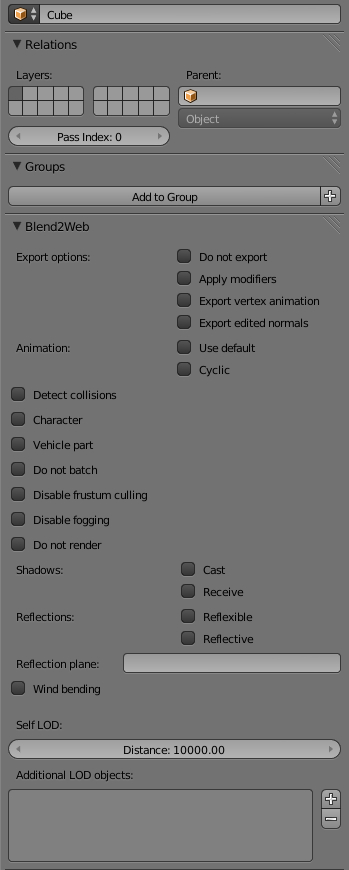
\includegraphics[width=0.600\linewidth]{object_setup.jpg}
\end{figure}
\begin{description}
\item[{\emph{Transform \textgreater{} Location}}] \leavevmode
Координаты местоположения.

\item[{\emph{Transform \textgreater{} Rotation}}] \leavevmode
Углы вращения. Должен быть выставлен режим по умолчанию \code{XYZ Euler}.

\item[{\emph{Transform \textgreater{} Scale}}] \leavevmode
Масштабирование. Все 3 компоненты (x, y, z) должны быть одинаковы. Для физических объектов масштабирование не поддерживается.

\item[{\emph{Object Data} (вкладка)}] \leavevmode
Указатель на блок данных, специфичный для объектов разного типа.

\item[{\emph{Relation \textgreater{} Parent}}] \leavevmode
Указатель на родительский объект.

\item[{\emph{Blend4Web \textgreater{} Do not export}}] \leavevmode
Не экспортировать.

\item[{\emph{Blend4Web \textgreater{} Apply modifiers}}] \leavevmode
Применить модификаторы объекта при экспорте.

\item[{\emph{Blend4Web \textgreater{} Export vertex animation}}] \leavevmode
Экспортировать предварительно созданную и сохраненную вертексную анимацию.

\item[{\emph{Blend4Web \textgreater{} Export edited normals}}] \leavevmode
Экспортировать предварительно отредактированные и сохраненные нормали.

\item[{\emph{Blend4Web \textgreater{} Animation \textgreater{} Use default}}] \leavevmode
Использовать по умолчанию связанную с объектом объектную или скелетную анимацию.

\item[{\emph{Blend4Web \textgreater{} Animation \textgreater{} Cyclic}}] \leavevmode
Циклически повторять связанную с объектом анимацию. Зацикливание анимации влияет также на анимацию системы частиц или спикера (в случае их присутствия).

\item[{\emph{Blend4Web \textgreater{} Detect collisions}}] \leavevmode
Активировать связанную с объектом физику.

\item[{\emph{Blend4Web \textgreater{} Character}}] \leavevmode
Активировать использование объекта в качестве физического каркаса игрового персонажа.

\item[{\emph{Blend4Web \textgreater{} Vehicle part}}] \leavevmode
Активировать использование объекта в качестве составной части транспортного средства.

\item[{\emph{Blend4Web \textgreater{} Do not batch}}] \leavevmode
Запретить комбинирование меша объекта с другими мешами, имеющими одинаковый материал, которое осуществляется в целях оптимизации количества вызовов отрисовки. Объекты, имеющие анимацию или физику, уже рассматриваются как отдельные. Опция применяется исключительно в случаях, когда необходимо обеспечить движение объекта, однако явным образом это не вытекает из имеющихся на нём опций.

\item[{\emph{Blend4Web \textgreater{} Disable frustum culling}}] \leavevmode
Отключить оптимизацию отсечением по зоне видимости.

\item[{\emph{Blend4Web \textgreater{} Disable fogging}}] \leavevmode
Отключить туман для объекта.

\item[{\emph{Blend4Web \textgreater{} Do not render}}] \leavevmode
Отключить рендеринг объекта (например, вспомогательный объект физики).

\item[{\emph{Blend4Web \textgreater{} Shadows: Cast} и \emph{Blend4Web \textgreater{} Shadows: Receive}}] \leavevmode
Отбрасывать и получать тени, соответственно. Могут быть включены одновременно.

\item[{\emph{Blend4Web \textgreater{} Reflections: Reflexible}}] \leavevmode
При включении объект будет отражаться от зеркальных поверхностей.

\item[{\emph{Blend4Web \textgreater{} Reflections: Reflective}}] \leavevmode
При включении объект будет отражать своей поверхностью другие объекты.

\item[{\emph{Blend4Web \textgreater{} Reflections: Reflection plane}}] \leavevmode
Текстовое поле для названия пустого объекта, задающего плоскость отражения.

\item[{\emph{Blend4Web \textgreater{} Wind bending}}] \leavevmode
Включить процедурную анимацию под действием ветра.

\item[{\emph{Blend4Web \textgreater{} Self LOD \textgreater{} Distance}}] \leavevmode
Расстояние от камеры, на котором объект перестает отображаться. Значение по умолчанию 10000.0.

\item[{\emph{Blend4Web \textgreater{} Additional LOD objects}}] \leavevmode
Интерфейс добавления низкополигональных объектов для реализации переключения уровня детализации.

\end{description}


\section{Управление перемещением}
\label{objects:id4}
Для управления перемещением объектов в движке предусмотрены следующие базовые функции модуля \emph{transform}:
\begin{description}
\item[{\emph{set\_translation, set\_translation\_v}}] \leavevmode
Переместить центр объекта в указанное место. Первая функция принимает в качестве параметров отдельные координаты, вторая - трёхмерный вектор (Array или Float32Array).

\item[{\emph{set\_rotation, set\_rotation\_v}}] \leavevmode
Установить кватернион поворота объекта. Первая функция принимает в качестве параметров отдельные координаты, вторая - четырёхмерный вектор (Array или Float32Array).

\item[{\emph{set\_scale}}] \leavevmode
Установить коэффициент увеличения объекта. Единица соответствует исходному состоянию. Значение меньше единицы - уменьшение. Значение больше единицы - увеличение. Не все объекты могут быть увеличены. В частности, увеличение невозможно для физических объектов.

\item[{\emph{get\_translation}}] \leavevmode
Получить координаты центра объекта. Вариант с одним параметром возвращает новый вектор (неоптимизированный варант), варант с двумя требует отдельного вектора для записи результата.

\item[{\emph{get\_rotation}}] \leavevmode
Получить кватернион поворота объекта. По аналогии с \emph{get\_translation} имеется два варианта вызова функции.

\item[{\emph{get\_scale}}] \leavevmode
Получить значение коэффициента увеличения объекта.

\end{description}


\section{Камера}
\label{objects:id5}
Настройки камеры выставляются в панели \code{Properties} на вкладке \code{Object Data}.

\emph{Blend4Web \textgreater{} Move style} -- исходный стиль управления камерой. По умолчанию камера
находится в статическом режиме (\code{Static}), допуская измененение своего
положения только через API. В режиме \code{Target} камера вращается вокруг
фиксированной точки. Режим \code{Eye} позволяет осуществлять вращение и перемещение от первого
лица.

\emph{Blend4Web \textgreater{} Target location} -- доступно в режиме \code{Target}. Позиция точки,
относительно которой будет вращаться камера. Кропка \code{Copy Cursor Location}
позволяет скопировать текущее положение курсора.

\emph{Blend4Web \textgreater{} Use distance limits} -- доступно в режиме \code{Target}. Ограничить
перемещение камеры двумя крайними расстояниями.

\emph{Blend4Web \textgreater{} Use vertical rotation clamping} -- доступно в режиме \code{Target} и \code{Eye}.
Ограничить вертикальный угол расположения камеры двумя крайними значениями.

\emph{Blend4Web \textgreater{} DOF front distance} -- описано в разделе {\hyperref[postprocessing_effects:postprocessing-effects]{\emph{Постпроцессинговые эффекты}}}

\emph{Blend4Web \textgreater{} DOF rear distance} -- описано в разделе {\hyperref[postprocessing_effects:postprocessing-effects]{\emph{Постпроцессинговые эффекты}}}

\emph{Blend4Web \textgreater{} DOF power} -- описано в разделе {\hyperref[postprocessing_effects:postprocessing-effects]{\emph{Постпроцессинговые эффекты}}}
\phantomsection\label{textures:textures}
\index{текстуры}

\chapter{Текстуры}
\label{textures:index-0}\label{textures::doc}\label{textures:id1}
\index{текстуры!типы}

\section{Типы текстур}
\label{textures:id2}\label{textures:index-1}
Опция выбора типа текстуры \code{Type} расположена во вкладке \code{Textures}. Движком поддерживаются текстуры следующих типов:
\begin{enumerate}
\item {} \begin{description}
\item[{\code{Image or Movie}, изображение или фильм}] \leavevmode\begin{itemize}
\item {} 
диффузная (diffuse map)

\item {} 
карта бликов (specular map), может также содержаться в альфа-канале диффузной текстуры

\item {} 
карта нормалей (normal map)

\item {} 
карта высот (height map), может содержатся только в альфа-канале карты нормалей, используется для реализации рельефной поверхности (parallax mapping)

\item {} 
карта прозрачности (alpha map) - применяется отдельно только для рендеринга воды в режиме совместимости, в обычном материале может содержаться в альфа-канале диффузной текстуры

\item {} 
карта смешивания (stencil map)

\end{itemize}

\end{description}

\item {} \begin{description}
\item[{\code{Environment Map}, карта окружения}] \leavevmode\begin{itemize}
\item {} 
карта зеркального отражения (mirror map)

\item {} 
{\hyperref[textures:skydome-texture]{\emph{текстура неба (skydome)}}}.

\end{itemize}

\end{description}

\item {} \begin{description}
\item[{\code{None}, пустая}] \leavevmode\begin{itemize}
\item {} 
применена на кубе в стартовой сцене Blender'a, в движке генерируется серая текстура. Также используется для {\hyperref[textures:render-to-texture]{\emph{рендеринга сцены в текстуру}}}.

\end{itemize}

\end{description}

\item {} \begin{description}
\item[{\code{Blend}, градиент}] \leavevmode\begin{itemize}
\item {} 
используется в {\hyperref[particles:particles-textures]{\emph{системах частиц}}}.

\end{itemize}

\end{description}

\item {} \begin{description}
\item[{\code{Voronoi}, процедурная текстура с разбиением Вороного}] \leavevmode\begin{itemize}
\item {} 
используется для рендеринга воды с целью настройки каустики

\end{itemize}

\end{description}

\end{enumerate}

\index{текстуры!настройки}

\section{Общие настройки}
\label{textures:id3}\label{textures:index-2}\begin{description}
\item[{\emph{Размер}}] \leavevmode
Размер растров для текстур-изображений (длина и ширина изображения в пикселах) должен быть числом 2$^{\text{N}}$, т.е. 4, 8, 16, 32, 64, 128, 256, 512, 1024, 2048, 4096 пикселов. Для корректной работы компрессии текстур размер должен составлять не менее 4 пикселов. Как правило, используются изображения квадратной формы (например, 512 x 512 px), однако могут использоваться и прямоугольные (например, 4 x 128 px). Использование изображений размером более 1024 пикселов не рекомендуется.

\item[{\emph{Image Mapping \textgreater{} Extension}}] \leavevmode
Режим интерпретации текстурных координат (в WebGL - Wrap Mode). Доступен для текстур типа \code{Image or Movie}. В случае значения \code{Repeat} движок устанавливает для текстуры режим \code{REPEAT}. При этом целочисленная часть текстурных координат игнорируется, используется только дробная часть. Во всех остальных случаях (например, \code{Extend}) движок устанавливает \code{CLAMP\_TO\_EDGE}. При этом происходит ограничение текстурных координат отрезком {[}0, 1{]}. Значение по умолчанию \code{Repeat}.

\end{description}

\index{material capture}\index{matcap}\begin{description}
\item[{\emph{Mapping \textgreater{} Coordinates}}] \leavevmode
Тип текстурных координат. Поддерживаются \code{UV} (использовать развертку), \code{Normal} (использовать направление на камеру, только для диффузных текстур, применяется для создания материалов в стиле \textbf{material capture}, \textbf{matcap}). Значение по умолчанию \code{Generated} (!).

\item[{\emph{Mapping \textgreater{} Offset}}] \leavevmode
Не поддерживается.

\item[{\emph{Mapping \textgreater{} Size}}] \leavevmode
Масштабирование развертки по соответствующим осям. Значения по умолчанию 1.0.

\item[{\emph{Blend4Web \textgreater{} Do not export}}] \leavevmode
Не экспортировать текстуру. По умолчанию отключено.

\item[{\emph{Blend4Web \textgreater{} Anisotropic Filtering}}] \leavevmode
Фактор анизотропной фильтрации для индивидуальной текстуры. Имеет приоритет перед аналогичной настройкой для сцены. Значение по умолчанию \code{DEFAULT} (т.е. использовать настройки сцены).

\item[{\emph{Blend4Web \textgreater{} UV translation velocity}}] \leavevmode
Скорость анимации текстурных координат по соответствующим осям. Значения по умолчанию 0.0.

\item[{\emph{Blend4Web \textgreater{} Water Foam}}] \leavevmode
Текстура пены. Используется материалом для рендеринга воды.

\end{description}

\index{текстуры!диффузная}\index{diffuse map}

\section{Диффузная текстура (diffuse map)}
\label{textures:index-4}\label{textures:diffuse-map}
Диффузная текстура применяется для указания распределения цвета рассеянного света (модель Ламберта).


\subsection{Активация}
\label{textures:id4}
Выставить опцию \code{Diffuse \textgreater{} Color} на панели \code{Textures \textgreater{} Influence}.


\subsection{Дополнительные настройки}
\label{textures:id5}\begin{description}
\item[{\emph{Influence \textgreater{} Diffuse \textgreater{} Color}}] \leavevmode
Степень влияния текстуры на диффузный цвет. Значение по умолчанию 1.0.

\item[{\emph{Influence \textgreater{} Blend}}] \leavevmode
Тип взаимодействия с цветом материала (\code{Material \textgreater{} Diffuse \textgreater{} Color}), или с вертексным цветом, если включена опция \code{Vertex Color Paint}. Поддерживаются \code{Mix} (смешивается с цветом), \code{Multiply} (умножается на цвет). Значение по умолчанию \code{Mix}.

\end{description}

\index{текстуры!карта бликов}\index{specular map}

\section{Карта бликов (specular map)}
\label{textures:index-5}\label{textures:specular-map}
Карта бликов применяется для указания распределения цвета отраженного света (модель Фонга).


\subsection{Активация}
\label{textures:id6}
Выставить опцию \code{Specular \textgreater{} Color} на панели \code{Textures \textgreater{} Influence} (опция \code{Specular \textgreater{} Intensity} не поддерживается).


\subsection{Дополнительные настройки}
\label{textures:id7}\begin{description}
\item[{\emph{Influence \textgreater{} Specular \textgreater{} Color}}] \leavevmode
Степень влияния текстуры на цвет отраженного света. Значение по умолчанию 1.0.

\item[{\emph{Influence \textgreater{} Blend}}] \leavevmode
Тип взаимодействия с цветом отраженного света материала (\code{Material \textgreater{} Specular \textgreater{} Color}). Поддерживается только \code{Mix} (смешивается с цветом). Значение по умолчанию \code{Mix}.

\end{description}

Карта бликов может быть упакована в альфа-канал диффузной текстуры в целях оптимизации. В этом случае для текстуры необходимо одновременно выставить опции \code{Diffuse \textgreater{} Color} и \code{Specular \textgreater{} Color}. Цветовой диапазон ограничен оттенками серого цвета.

\index{текстуры!карта нормалей}\index{normal map}

\section{Карта нормалей (normal map)}
\label{textures:index-6}\label{textures:normal-map}
Карта нормалей применяется для указания распределения нормалей (перпендикуляров) к поверхности с целью увеличения уровня детализации ее рельефа. Информация о нормалях должна храниться в текстурном пространстве координат. Карты нормалей в объектном пространстве не поддерживаются.


\subsection{Активация}
\label{textures:id8}
Выставить опцию \code{Geometry \textgreater{} Normal} на панели \code{Textures \textgreater{} Influence}.


\subsection{Дополнительные настройки}
\label{textures:id9}\begin{description}
\item[{\emph{Influence \textgreater{} Geometry \textgreater{} Normal}}] \leavevmode
Степень участия карты в расчетах нормалей. Значение по умолчанию 1.0.

\end{description}

\index{текстуры!карта высот}\index{height map}\index{parallax mapping}

\section{Карта высот (height map). Parallax mapping}
\label{textures:index-7}\label{textures:height-map-parallax-mapping}
Карта высот содержит информацию о распределении относительных высот рельефа. Более высокий уровень поверхности обозначается более светлым цветом. Карта высот в сочетании с картой нормалей требуются в качестве входящих данных для реализации рельефной поверхности (parallax mapping). Карта высот должна содержатся в альфа-канале карты нормалей.


\subsection{Активация}
\label{textures:id10}
Для карты нормалей дополнительно к опции \code{Geometry \textgreater{} Normal} на панели \code{Textures \textgreater{} Influence} выставить опцию \code{Parallax} на панели \code{Textures \textgreater{} Blend4Web}.


\subsection{Дополнительные настройки}
\label{textures:id11}\begin{description}
\item[{\emph{Blend4Web \textgreater{} Parallax Scale}}] \leavevmode
Фактор влияния эффекта рельефной поверхности. Значение по умолчанию 0.03.

\item[{\emph{Blend4Web \textgreater{} Parallax Steps}}] \leavevmode
Количество итераций в расчетах рельефной поверхности. Большее значение приводит к лучшему качеству и к большим затратам вычислительных ресурсов. Значение по умолчанию 10.

\end{description}

{\hfill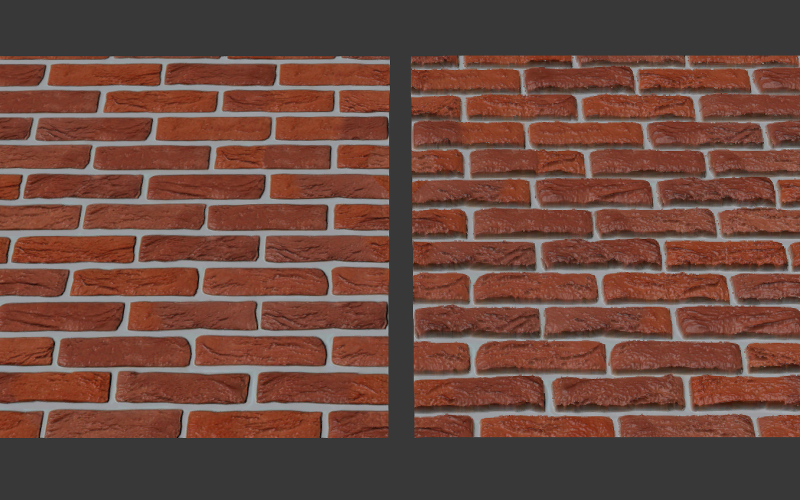
\includegraphics[width=1.000\linewidth]{parallax.jpg}\hfill}

\begin{DUlineblock}{0em}
\item[] 
\end{DUlineblock}

\index{текстуры!карта прозрачности}\index{alpha map}

\section{Карта прозрачности (alpha map)}
\label{textures:alpha-map}\label{textures:texture-alpha-map}\label{textures:index-8}
Отдельная карта прозрачности применяется только для воды в режиме совместимости. В обычном материале может содержаться в альфа-канале диффузной текстуры.


\subsection{Активация}
\label{textures:id12}
Для диффузной текстуры дополнительно к опции \code{Diffuse \textgreater{} Color} на панели \code{Textures \textgreater{} Influence} выставить опцию \code{Diffuse \textgreater{} Alpha}. Для отдельной карты прозрачности выставить опцию \code{Diffuse \textgreater{} Alpha}.


\subsection{Дополнительные настройки}
\label{textures:id13}\begin{description}
\item[{\emph{Influence \textgreater{} Diffuse \textgreater{} Alpha}}] \leavevmode
Не поддерживается.

\item[{\emph{Influence \textgreater{} Blend}}] \leavevmode
Не поддерживается.

\end{description}

{\hfill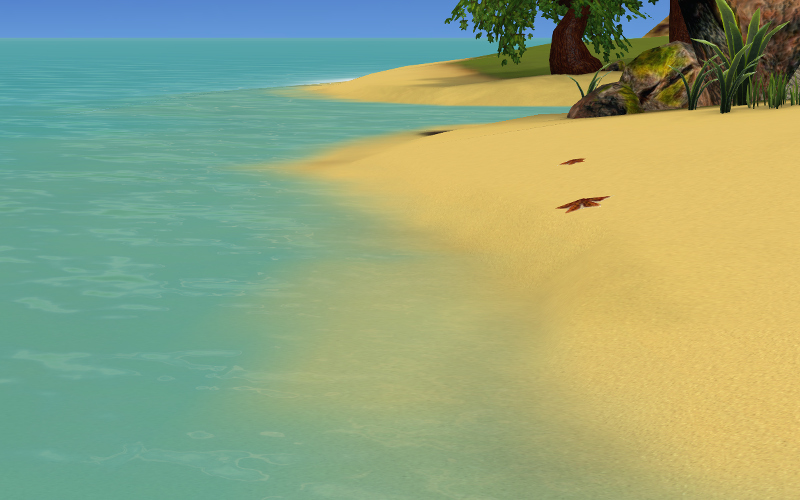
\includegraphics[width=1.000\linewidth]{alpha_map_water.jpg}\hfill}

\begin{DUlineblock}{0em}
\item[] 
\end{DUlineblock}

\index{текстуры!карта смешивания}\index{stencil map}

\section{Карта смешивания (stencil map)}
\label{textures:stencil-map}\label{textures:index-9}
Специальная текстура (цветная или оттенков серого), содержащая информацию о распределении других текстур по поверхности.


\subsection{Активация}
\label{textures:id14}\begin{enumerate}
\item {} 
В случае нодовых материалов карта смешивания должна использоваться соответствующим образом в нодовой структуре.

\item {} 
В случае обычных материалов карта смешивания должна располагаться в текстурном слоте между двумя смешиваемыми диффузными текстурами. Для текстуры смешивания необходимо одновременно выставить опции \code{RGB to Intensity} и \code{Stencil} на панели \code{Textures \textgreater{} Influence}.

\end{enumerate}


\subsection{Дополнительные настройки}
\label{textures:id15}
В случае обычных материалов для одной из смешиваемых диффузных текстур поддерживается тип текстурных координат \code{Normal} (``matcap'').


\subsection{Ограничения}
\label{textures:id16}
В случае обычных материалов движком интерпретируется только красный канал текстуры смешивания. Карта бликов или карта нормалей при их наличии смешиванию не подвергаются. Настройка масштабирования \code{Mapping \textgreater{} Size} извлекается из первой текстуры и применяется ко всем остальным текстурам.


\subsection{Пример}
\label{textures:id17}
Материал яблока имеет текстуры: карту нормалей, диффузную текстуру с картой бликов в альфа-канале, карту смешивания, диффузную карту ``matcap'', карту зеркального отражения.

{\hfill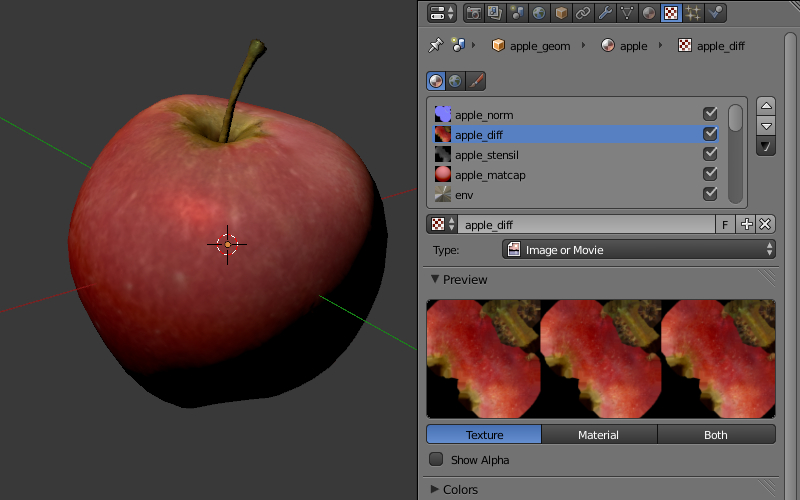
\includegraphics[width=1.000\linewidth]{stencil_apple.jpg}\hfill}

\begin{DUlineblock}{0em}
\item[] 
\end{DUlineblock}

{\hfill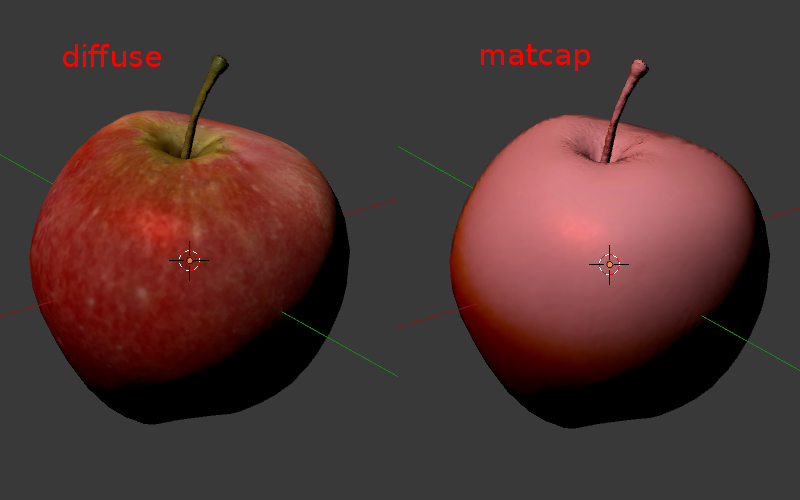
\includegraphics[width=1.000\linewidth]{stencil_apple_separate_textures.jpg}\hfill}

\begin{DUlineblock}{0em}
\item[] 
\end{DUlineblock}

\index{текстуры!карта окружения}\index{environment map}

\section{Карта окружения (environment map)}
\label{textures:environment-map}\label{textures:index-10}
Применяется в качестве карты зеркального отражения (mirror map) и в качестве статической текстуры неба (skydome).

В движке представлена кубической текстурой. Растры для карт окружения должны содержать 6 спроецированных изображений окружающей среды, упакованных в 2 ряда по 3 (формат, используемый в Blender'e). Размер растров для каждого из изображений должен подчиняться правилу 2$^{\text{N}}$ (512, 1024 и т.п.).

Во избежания проявления швов рекомендуется использовать формат без потери качества (PNG).

{\hfill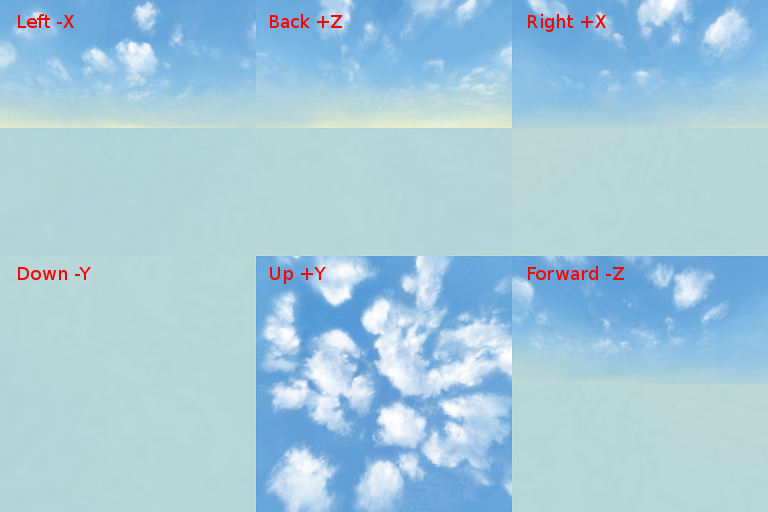
\includegraphics[width=1.000\linewidth]{environment_map.png}\hfill}


\subsection{Создание карты окружения}
\label{textures:id18}
Blender позволяет запекать сцену в карту окружения. Для этого:
\begin{enumerate}
\item {} 
Создать сцену для запекания.

\item {} 
Добавить пустой объект в предполагаемом центре обзора (\code{Add \textgreater{} Empty}).

\item {} 
Перейти во вкладку \code{World}, затем перейти во вкладку \code{Textures}, создать новую текстуру, выбрать тип \code{Environment Map}.

\item {} 
На панели \code{Environment Map} выбрать источник \code{Static}, выбрать созданный пустой объект в поле \code{Viewport Object}, установить разрешение 2$^{\text{N}}$ (512, 1024 и т.п.).

\item {} 
Выполнить рендеринг сцены \code{F12} (требуется наличие камеры).

\item {} 
Сохранить карту окружения в файл.

\end{enumerate}

{\hfill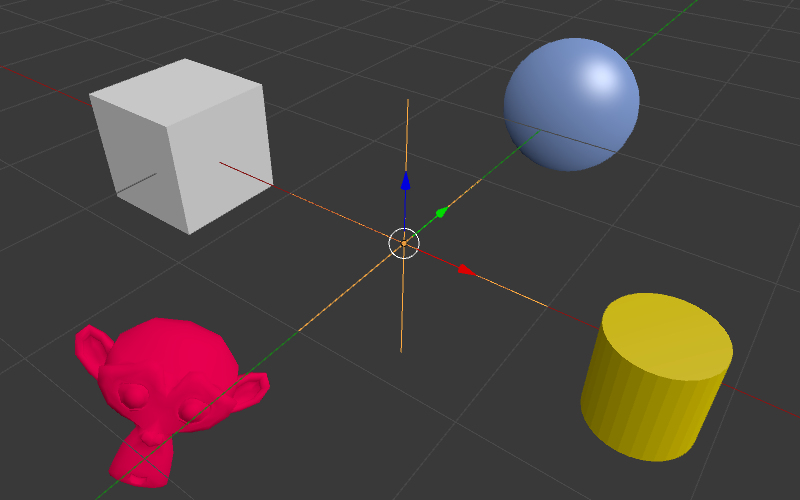
\includegraphics[width=1.000\linewidth]{environment_map_baking_scene.jpg}\hfill}

\begin{DUlineblock}{0em}
\item[] 
\end{DUlineblock}

{\hfill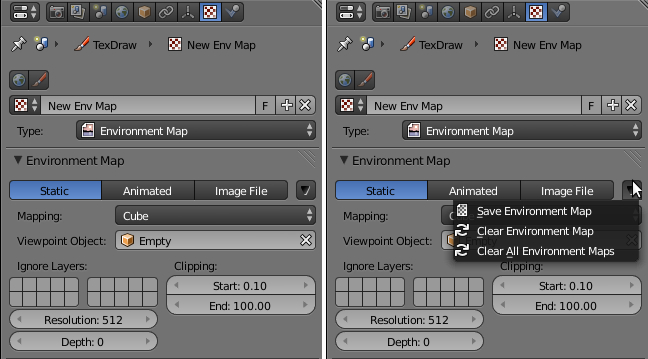
\includegraphics[width=1.000\linewidth]{environment_map_baking_ui.jpg}\hfill}

\index{текстуры!карта зеркального отражения}\index{mirror map}

\section{Карта зеркального отражения (mirror map)}
\label{textures:id19}\label{textures:mirror-map}\label{textures:index-11}
Применяется для визуализации отражающей способности поверхности. Представляет собой карту окружения.


\subsection{Активация}
\label{textures:id20}
Выбрать тип текстуры (\code{Type}) \code{Environment Map}. Выставить опцию \code{Shading \textgreater{} Mirror} на панели \code{Textures \textgreater{} Influence}.


\subsection{Дополнительные настройки}
\label{textures:id21}\begin{description}
\item[{\emph{Influence \textgreater{} Shading \textgreater{} Mirror}}] \leavevmode
Степень влияния карты зеркального отражения текстуры. Значение по умолчанию 1.0.

\end{description}


\strong{See also:}


{\hyperref[materials:reflection-static]{\emph{Статическое отражение}}}.



\index{текстуры!небо}\index{skydome}

\section{Текстура неба (skydome)}
\label{textures:skydome}\label{textures:skydome-texture}\label{textures:index-12}
Применяется для визуализации небесного свода. Представляет собой карту окружения.


\subsection{Активация}
\label{textures:id22}
Создать специальным образом ориентированную плоскость. Создать метериал, выставить опцию \code{Blend4Web \textgreater{} Special: Skydome}. Создать текстуру типа \code{Environment Map}.


\subsection{Дополнительные настройки}
\label{textures:id23}
Во избежания исчезновения изображения при поворотах камеры для объекта плоскости выставить опцию \code{Blend4Web \textgreater{} Disable frustum culling}.

{\hfill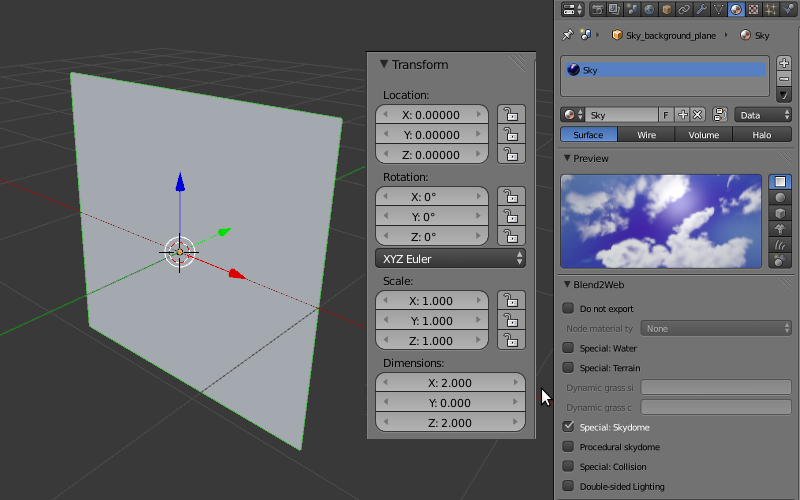
\includegraphics[width=1.000\linewidth]{skydome.jpg}\hfill}

\begin{DUlineblock}{0em}
\item[] 
\end{DUlineblock}
\phantomsection\label{textures:render-to-texture}
\index{текстуры!рендеринг в}\index{render-to-texture}\index{RTT}

\section{Рендеринг в текстуру (render-to-texture, RTT)}
\label{textures:render-to-texture-rtt}\label{textures:index-13}
Изображение 3D сцены может быть использовано в качестве текстуры на объекте другой (``главной'') сцены.


\subsection{Активация}
\label{textures:id24}\begin{enumerate}
\item {} 
Создать дополнительную сцену-источник, переименовать для удобства, создать \code{World}, добавить нужные объекты, настроить вид из камеры.

\item {} 
В главной сцене для текстуры целевого объекта выставить тип \code{None}, в поле \code{Blend4Web \textgreater{} Source scene} указать название сцены-источника. В меню \code{Mapping \textgreater{} Coordinates} выбрать \code{UV}.  Убедиться, что меш объекта имеет развертку.

\end{enumerate}

{\hfill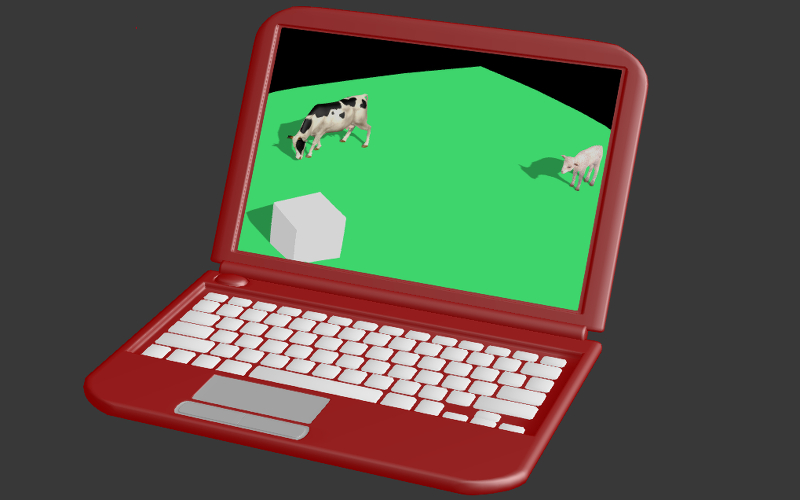
\includegraphics[width=1.000\linewidth]{render_to_texture.jpg}\hfill}


\subsection{Ограничения}
\label{textures:id25}
В настоящее время имеется баг, вынуждающий иметь в обеих сценах один общий источник света.
\phantomsection\label{materials:materials}
\index{материалы}

\chapter{Материалы}
\label{materials:index-0}\label{materials::doc}\label{materials:id1}
Материалы описывают реакцию поверхности объекта на освещение, а также содержат информацию о ее прозрачности, отражающей способности, физических и других параметрах.

Меши могут использовать один или несколько материалов. В случае использования нескольких материалов назначение их различным полигонам происходит в режиме редактирования \code{Edit Mode}. Для этого нужно выделить нужные полигоны, выбрать материал из списка и нажать кнопку \code{Assign}.

Поддерживаются следующие типы материалов: \code{Surface} (поверхность), \code{Halo} (гало).

\index{материалы!параметры освещения}

\section{Параметры освещения}
\label{materials:id2}\label{materials:index-1}\label{materials:material-lighting-params}\begin{figure}[htbp]
\centering

\scalebox{0.500000}{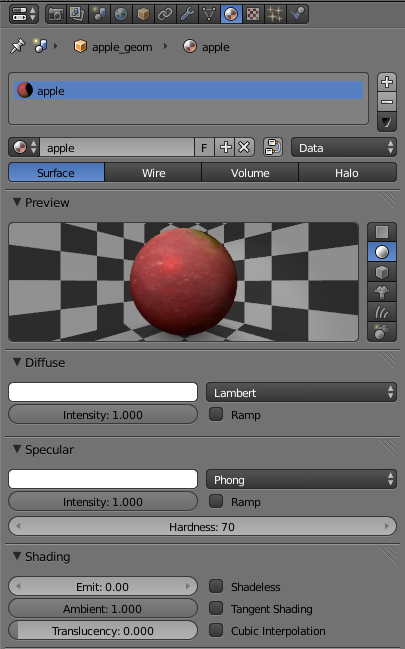
\includegraphics{material_panel_shading.jpg}}
\end{figure}
\begin{description}
\item[{\emph{Diffuse \textgreater{} Color}}] \leavevmode
Цвет диффузного (рассеянного) света. Значение по умолчанию (0.8, 0.8, 0.8). Может взаимодействовать с цветом диффузной текстуры.

\item[{\emph{Diffuse \textgreater{} Intensity}}] \leavevmode
Интенсивность диффузного (рассеянного) света. Значение по умолчанию 0.8.

\item[{\emph{Diffuse \textgreater{} Shader}}] \leavevmode
Алгоритм расчета диффузного (рассеянного) освещения. Игнорируется движком. В движке используется алгоритм Ламберта (\code{Lambert}). Значение по умолчанию \code{Lambert}.

\item[{\emph{Specular \textgreater{} Color}}] \leavevmode
Цвет отраженного света. Значение по умолчанию (1.0, 1.0, 1.0). Может взаимодействовать с цветом карты бликов.

\item[{\emph{Specular \textgreater{} Intensity}}] \leavevmode
Интенсивность отраженного света. Значение по умолчанию 0.5.

\item[{\emph{Specular \textgreater{} Hardness}}] \leavevmode
Степенной показатель в формуле расчета отраженного света (``жесткость'' блика). Значение по умолчанию 50. Алгоритм применения в движке отличается от алгоритма применения в Blender'e.

\item[{\emph{Specular \textgreater{} Shader}}] \leavevmode
Алгоритм расчета отраженного освещения. Игнорируется движком. В движке используется алгоритм Фонга (\code{Phong}). Значение по умолчанию \code{CookTorr}.

\item[{\emph{Shading \textgreater{} Emit}}] \leavevmode
Интенсивность эмиссии (излучения). Значение по умолчанию 0.0.

\item[{\emph{Shading \textgreater{} Ambient}}] \leavevmode
Фактор влияния освещения от окружающей среды на материал. Значение по умолчанию 1.0.

\item[{\emph{Shading \textgreater{} Shadeless}}] \leavevmode
При включении материал не реагирует на освещение. По умолчанию выключено.

\item[{\emph{Game Settings \textgreater{} Backface Culling}}] \leavevmode
При включении обратная сторона полигона не отображается движком. По умолчанию включено.

\item[{\emph{Options \textgreater{} Vertex Color Paint}}] \leavevmode
Опция включает использование вертексного цвета меша вместо диффузного цвета.

\end{description}

\index{материалы!прозрачность}\index{прозрачность}

\section{Прозрачность}
\label{materials:id3}\label{materials:index-2}
\index{прозрачность!типы}

\subsection{Типы}
\label{materials:id4}\label{materials:index-3}
Тип реализации прозрачности выбирается в меню \code{Alpha Blend} на панели \code{Materials \textgreater{} Game Settings} (в режиме \code{Blender Game}).

Движком поддерживаются следующие типы реализации прозрачности, перечисленные в порядке увеличения производительности:
\begin{description}
\item[{\emph{Alpha Sort}}] \leavevmode
Прозрачный с градиентом. Для корректного отображения перекрывания одних прозрачных поверхностей другими движком производится сортировка треугольников по дальности от камеры. Операция требует дополнительных затрат вычислительных ресурсов. Рекомендуется применять для замкнутых прозрачных объектов (бутылка, стекла автомобиля и т.д.).

\item[{\emph{Alpha Blend}}] \leavevmode
Прозрачный с градиентом. Сортировка треугольников не производится. Рекомендуется применять для незамкнутых прозрачных объектов (поверхность воды, декали).

\item[{\emph{Add}}] \leavevmode
Прозрачный c градиентом. Сортировка треугольников не производится. Движок отключает запись в буфер глубины, что приводит к произвольному порядку отображения прозрачных поверхностей. Рекомендуется применять для создания эффектов (системы частиц, светящиеся лучи).

\item[{\emph{Alpha Clip}}] \leavevmode
Прозрачный без градиента. Движок отбрасывает пикселы (discard) с прозрачностью менее 0.5. Сортировка треугольников не производится. Рекомендуется применять с текстурой в качестве маски для визуализации множества мелких деталей (листва деревьев, трава).

\item[{\emph{Opaque}}] \leavevmode
Непрозрачный. Значение по умолчанию.

\end{description}

{\hfill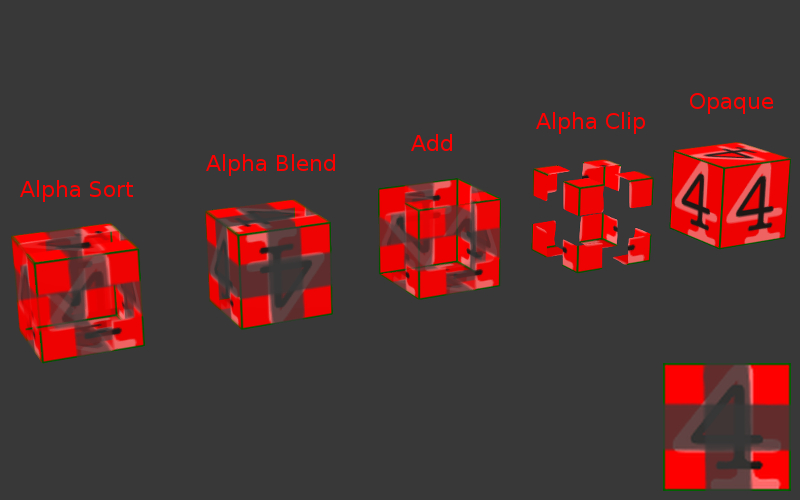
\includegraphics[width=1.000\linewidth]{alpha_types.jpg}\hfill}

\index{прозрачность!настройка}

\subsection{Дополнительные настройки}
\label{materials:index-4}\label{materials:id5}\begin{description}
\item[{\emph{Transparency}}] \leavevmode
Опция включения прозрачности требуется для отображения прозрачных объектов в Blender'e. Движок игнорирует эту опцию, используя вместо нее \code{Alpha Blend}.

\item[{\emph{Transparency \textgreater{} Alpha}}] \leavevmode
Уровень прозрачности материала. При наличии диффузной текстуры движок (в отличие от Blender'a) игнорирует этот параметр, используя вместо него значение прозрачности текстуры.

\item[{\emph{Options \textgreater{} Z Offset}, смещение по глубине}] \leavevmode
Используется для явного указания расположения прозрачных объектов с \textbf{разными} материалами относительно друг друга с целью сортировки по глубине. Может принимать отрицательные и положительные значения. Для корректного отображения дальние объекты должны иметь меньшее значение параметра, чем ближние. Значение по умолчанию 0.0.

\item[{\emph{Transparency \textgreater{} Fresnel}}] \leavevmode
Степень Френеля для прозрачности. Экспортируется, но в настоящее время не используется.

\item[{\emph{Transparency \textgreater{} Blend}}] \leavevmode
Фактор Френеля для прозрачности. Экспортируется, но в настоящее время не используется.

\end{description}

\index{материалы!зеркальное отражение}\index{зеркальное отражение}

\section{Зеркальное отражение}
\label{materials:id6}\label{materials:index-5}\label{materials:material-mirror}
\index{зеркальное отражение!статическое}

\subsection{Статическое отражение}
\label{materials:id7}\label{materials:index-6}\label{materials:reflection-static}
Поверхность отражает одно и то же изображение вне зависимости от изменения окружающей среды. Для активации достаточно использовать {\hyperref[textures:mirror-map]{\emph{карту зеркального отражения}}}.


\strong{See also:}


{\hyperref[materials:fresnel]{\emph{Эффект Френеля для отражения}}}



\index{зеркальное отражение!динамическое}

\subsection{Динамическое отражение}
\label{materials:index-7}\label{materials:id8}
Поверхность отражает текущее расположение определенных объектов. Поддерживается только отражение от плоскости.


\subsubsection{Активация}
\label{materials:id9}\begin{enumerate}
\item {} 
Включить опцию \code{Render reflections} на панели \code{Scene \textgreater{} Blend4Web}.

\item {} 
Добавить пустой объект для задания плоскости отражения \code{Add \textgreater{} Empty \textgreater{} Single Arrow}. Переименовать для удобства.

\item {} 
Для \emph{отражающих} объектов на панели \code{Object \textgreater{} Blend4Web} выставить опцию \code{Reflective} и указать имя пустого объекта в поле \code{Reflection plane}.

\item {} 
Для нужных материалов \emph{отражающих} объектов выставить значение отражающей способности \code{Mirror \textgreater{} Reflectivity}.

\item {} 
Для \emph{отражаемых} объектов на панели \code{Object \textgreater{} Blend4Web} выставить опцию \code{Reflexible}.

\end{enumerate}

\begin{notice}{note}{Note:}
Рекомендуется также включить использование освещения от окружающей среды \code{World \textgreater{} Environment Lighting}.
\end{notice}


\subsubsection{Ограничения}
\label{materials:id10}
В отраженном изображении игнорируется карта нормалей, тени.


\strong{See also:}


{\hyperref[materials:fresnel]{\emph{Эффект Френеля для отражения}}}



\index{зеркальное отражение!эффект Френеля}\index{эффект Френеля}

\subsection{Эффект Френеля для отражения}
\label{materials:id11}\label{materials:fresnel}\label{materials:index-8}
Эффект Френеля проявляется в зависимости интенсивностей проходящего и отраженного света от угла падения. Если угол падения близок к нулю (т.е. свет падает почти перпедикулярно поверхности), доля проходящего света велика, а отраженного мала. И наоборот, если угол падения близок к 90 градусам (т.е. свет падает почти параллельно поверхности), отражается почти весь свет.

Движок использует приближенную формулу Шлика:
\begin{quote}

R = R$_{\text{0}}$ + (1 − R$_{\text{0}}$)(1 - cos \(\theta\))$^{\text{N}}$, где

R - коэффициент отражения,

R$_{\text{0}}$ - коэффициент отражения в случае обзора под прямым углом к поверхности (т.е. при \(\theta\) = 0),

\(\theta\) - угол падения (равный углу отражения, под которым свет попадает в камеру), рассчитывается движком,

N - показатель степени.
\end{quote}


\subsubsection{Настройка}
\label{materials:id12}
Эффект Френеля применяется как для статического, так и для динамического отражения.
\begin{description}
\item[{\emph{Mirror \textgreater{} Fresnel}}] \leavevmode
Степень Френеля для отражения. Показатель степени N в формуле Шлика. В пакете Blender ограничен значениями от 0 до 5. Если этот параметр равен нулю, эффект Френеля не проявляется, происходит \emph{полное} отражение на всех углах. Если этот параметр больше нуля, при обзоре поверхности под углами, близкими к прямому (почти перпендикулярно поверхности), материал становится менее отражающим. Чем больше этот параметр, тем больше отклонение угла от прямого, для которого наблюдается такой эффект.

\item[{\emph{Mirror \textgreater{} Blend}}] \leavevmode
Фактор Френеля для отражения. Приводится к R$_{\text{0}}$ в формуле Шлика: R$_{\text{0}}$ = 1 - \code{Blend} / 5. В пакете Blender ограничен значениями от 0 до 5. Этот параметр показывает интенсивность проявления эффекта Френеля: чем больше фактор \code{Blend}, тем сильнее влияние эффекта Френеля. Если он равен нулю, эффект Френеля не проявляется.

\end{description}

{\hfill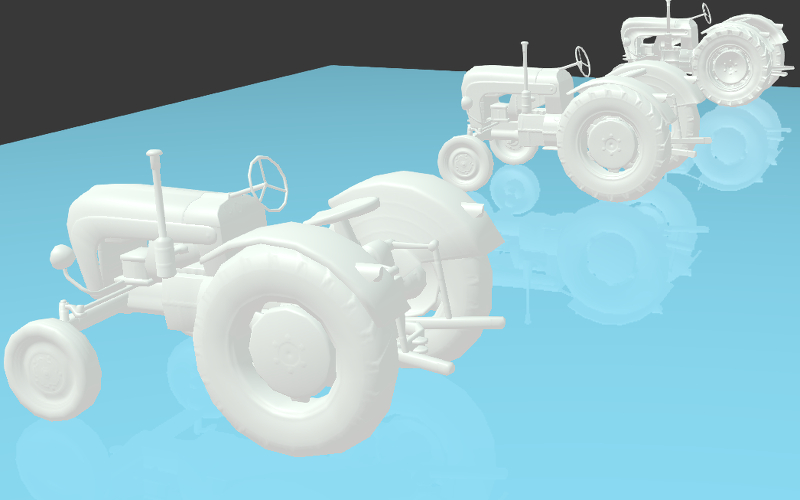
\includegraphics[width=1.000\linewidth]{reflection_dynamic_and_fresnel.jpg}\hfill}

\begin{DUlineblock}{0em}
\item[] 
\end{DUlineblock}

\index{материалы!специальные параметры}

\section{Специальные параметры движка}
\label{materials:id13}\label{materials:index-9}
Располагаются в панели \code{Blend4Web}.
\begin{description}
\item[{\emph{Do not export}}] \leavevmode
Не экспортировать.

\item[{\emph{Special: Water}}] \leavevmode
Специальный материал для рендеринга воды.

\item[{\emph{Special: Skydome}}] \leavevmode
Специальный материал для рендеринга неба.


\strong{See also:}


{\hyperref[textures:skydome-texture]{\emph{Текстура неба (skydome)}}}



\item[{\emph{Special: Collision}}] \leavevmode
Специальный материал для физического объекта.


\strong{See also:}


{\hyperref[physics:physics]{\emph{Физика}}}



\item[{\emph{Double-sided Lighting}}] \leavevmode
Включить двухстороннее освещение. Опция полезна для однослойных непросвечивающих объектов.

\end{description}

\index{материалы!гало}\index{halo}

\section{Материалы гало (Halo)}
\label{materials:material-halo}\label{materials:index-10}\label{materials:halo}
Используются в системах частиц и в статических мешах. Ниже рассматривается использование гало на статических мешах.


\subsection{Активация}
\label{materials:id14}
Выставить тип \code{Halo} во вкладке \code{Materials}. Рекомендуется также выставить тип прозрачности c градиентом (\code{Add}, \code{Alpha Blend} или \code{Alpha Sort}).

{\hfill
\includegraphics[width=1.000\linewidth]{halo.jpg}\hfill}


\subsection{Дополнительные настройки}
\label{materials:id15}\begin{description}
\item[{\emph{Halo \textgreater{} Alpha}}] \leavevmode
Параметр прозрачности материала. Значение по умолчанию 1.0 (непрозрачный).

\item[{\emph{Halo \textgreater{} Color}}] \leavevmode
Цвет материала. Значение по умолчанию (0.8, 0.8, 0.8) (почти белый).

\item[{\emph{Halo \textgreater{} Seed}}] \leavevmode
Не используется.

\item[{\emph{Halo \textgreater{} Size}}] \leavevmode
Размер частиц. Значение по умолчанию 0.5.

\item[{\emph{Halo \textgreater{} Hardness}}] \leavevmode
Показатель степени при расчете градиента. Влияет на видимый размер частиц. Значение по умолчанию 50.

\item[{\emph{Halo \textgreater{} Add}}] \leavevmode
Не используется.

\item[{\emph{Halo \textgreater{} Rings}}] \leavevmode
Использовать кольца. Настраивается относительное количество и цвет.

\item[{\emph{Halo \textgreater{} Lines}}] \leavevmode
Использовать линии. Настраивается относительное количество и цвет.

\item[{\emph{Halo \textgreater{} Star Tips}}] \leavevmode
Использовать звезды. Настраивается количество концов.

\item[{\emph{Blend4Web \textgreater{} Special: Stars}}] \leavevmode
Включает режим рендеринга звездного неба, при этом меш неподвижен относительно камеры. Для лампы необходимо также выставить опцию \code{Blend4Web \textgreater{} Dynamic intensity}. Приложения должны установить ночное время суток.

\item[{\emph{Blend4Web \textgreater{} Blending Height}}] \leavevmode
Диапазон высот, на котором происходит затухание яркости звезд.

\item[{\emph{Blend4Web \textgreater{} Stars Minimum Height}}] \leavevmode
Минимальная высота в локальном пространстве объекта, на которой видны звезды.

\end{description}
\phantomsection\label{node_materials:node-materials}
\index{нодовые материалы}

\chapter{Нодовые материалы}
\label{node_materials:index-0}\label{node_materials::doc}\label{node_materials:id1}
Шейдерные ноды (Shader Nodes) существенно расширяют возможности стандартных материалов Blender, позволяя представить освещение как серию базовых преобразований.

\index{материалы!ноды!}

\section{Стандартные ноды}
\label{node_materials:id2}\label{node_materials:index-1}\label{node_materials:generic-node-materials}
\index{материалы!ноды!}
Полностью поддерживается все возможности Blender, за исключением следующих случаев:
\begin{itemize}
\item {} 
\code{Geometry} - не поддерживаются выходы \code{Local}, \code{Orco} и \code{Vertex Alpha}.

\item {} 
\code{Material}, \code{Extended Material} - допускается не больше одной ноды на материал,
не поддерживаются входы \code{Refl}, \code{Ambient}, \code{SpecTra}, \code{Ray Mirror} и выход \code{AO}.

\item {} 
\code{RGB Curves} - не поддерживается.

\item {} 
\code{Vector Curves} - не поддерживается.

\end{itemize}

Кроме того, в контексте рендеринга в реальном времени, следует учитывать низкую производительность некоторых нод. Не рекомендуется к использованию:
\begin{itemize}
\item {} 
\code{Hue/Saturation}

\item {} 
\code{MixRGB} типы \code{Burn}, \code{Dodge}, \code{Value}, \code{Saturation}, \code{Hue}, \code{Color}

\end{itemize}

Не рекомендуется создавать сложные материалы, особенно использующие большое
количество нод \code{Geometry} и \code{Texture}.


\section{Дополнительные ноды}
\label{node_materials:custom-node-materials}\label{node_materials:id3}
\index{материалы!ноды!}
Дополнительные ноды расширяют функционал стандартных с учётом специфики работы движка. Ноды оформляются в виде нодовых групп (\code{Node groups} или \code{Node tree}) со специально выбранным именем и форматом входов. Для удобства, все дополнительные ноды собраны в файл \code{special\_nodes.blend}.


\subsection{LINEAR\_TO\_SRGB и LINEAR\_TO\_SRGB}
\label{node_materials:linear-to-srgb-linear-to-srgb}
Преобразование цвета из линейного цветового пространства в пространство sRGB и наоборот.


\strong{See also:}


{\hyperref[gamma_alpha:gamma-nodes]{\emph{Коррекция в нодовых материалах}}}




\subsection{REPLACE}
\label{node_materials:replace}
Осуществляет замену входов в зависимости от того, в какой среде работает в данный момент работает текущая сцена. При работе в Blender вход \code{Color1} подключается к выходу \code{Color}, вход \code{Color2} игнорируется. При работе в движке входы меняются местами (\code{Color1} игнорируется, \code{Color2} подключается к выходу).


\subsection{CLAMP}
\label{node_materials:clamp}
Осуществить операцию ограничения над входом. В результате, все элементы вектора на выходе
получают значения от 0 до 1 включительно.


\subsection{NORMAL\_VIEW}
\label{node_materials:normal-view}
Осуществить преобразование нормали в пространство камеры. Преобразование необходимо, поскольку при работе в движке все нормали определены в мировой системе координат. Нормаль используется только для наложения эффектов и не должна подключаться к входу ноды \code{Material} или \code{Extended Material}.


\subsection{PARALLAX}
\label{node_materials:parallax}
Реализует смещение текстурных координат в соответствии с картой высот.


\subsubsection{Входные параметры}
\label{node_materials:id4}\begin{description}
\item[{\emph{UV}}] \leavevmode
Исходные текстурные координаты.

\item[{\emph{Height}}] \leavevmode
RGBA текстура с картой высот в альфа канале.

\item[{\emph{Scale}}] \leavevmode
Коэффициент смещения текстурных координат.

\item[{\emph{Steps}}] \leavevmode
Количество шагов при генерации смещенных текстурных координат. Чем больше данное значение, тем выше качество получаемой текстуры.

\end{description}


\subsubsection{Выходные параметры}
\label{node_materials:id5}\begin{description}
\item[{\emph{UV}}] \leavevmode
Измененные текстурные координаты, которые используются как вход для текстурных нод.

\end{description}


\subsection{TRANSLUCENCY}
\label{node_materials:translucency}
Реализует эффект полупрозрачности (только по отношению к источникам света) для тонких объектов, таких как ткань, листва, бумага и др. Эффект состоит из двух частей: засвечивание обратной по отношению к источнику стороны объекта и появление светового пятна непосредственно в том месте, где должен был находится источник.


\subsubsection{Входные параметры}
\label{node_materials:id6}\begin{description}
\item[{\emph{Color}}] \leavevmode
Одноканальная текстура, определяющая неоднородность материала, белый - максимальный эффект просвечивания, черный - его отсутствие. По умолчанию используется белый.

\item[{\emph{Backside Factor}}] \leavevmode
Коэффицент коррекции цвета материала на обратной от источника света стороне. Основан на визуальном эффекте большей насыщенности цвета при просвечивании.
\begin{itemize}
\item {} 
\emph{Backside Factor \textless{} 1} - коррекция в сторону осветления

\item {} 
\emph{Backside Factor = 1} - без коррекции

\item {} 
\emph{Backside Factor \textgreater{} 1} - коррекция в сторону затемнения

\end{itemize}

Значение по умолчанию: 1.

\item[{\emph{Spot Hardness}}] \leavevmode
\begin{DUlineblock}{0em}
\item[] Коэффициент размытия светового пятна. При увеличении размеры пятна уменьшаются, края становятся более резкими.
\item[] Значение по умолчанию: 1000.
\end{DUlineblock}

\item[{\emph{Spot Intensity}}] \leavevmode
\begin{DUlineblock}{0em}
\item[] Интенсивность светового пятна. При увеличении становится более ярким.
\item[] Значение по умолчанию: 1.
\end{DUlineblock}

\item[{\emph{Spot Diffuse Factor}}] \leavevmode
Коэффициент влияния диффузного цвета материала на цвет светового пятна.
\begin{itemize}
\item {} 
\emph{Spot Diffuse Factor = 0} - световое пятно имеет диффузный цвет

\item {} 
\emph{Spot Diffuse Factor = 1} - световое пятно имеет белый цвет

\end{itemize}

Значение по умолчанию: 1.

\end{description}


\subsubsection{Выходные параметры}
\label{node_materials:id7}\begin{description}
\item[{\emph{Translucency}}] \leavevmode
Выход должен быть подключен ко входу \code{Translucency} ноды \code{Extended Material}.

\end{description}
\phantomsection\label{lighting:lighting}
\index{освещение}

\chapter{Освещение и тени}
\label{lighting:index-0}\label{lighting::doc}\label{lighting:id1}
\index{источники света}

\section{Освещение от источников света}
\label{lighting:id2}\label{lighting:index-1}
На сцене может быть несколько (но не менее одного) источников света разного типа.


\subsection{Типы источников света}
\label{lighting:id3}
Поддерживаются источники света следующих типов:
\begin{description}
\item[{\emph{Point}}] \leavevmode
Точечный. Свет распространяется из одной точки равномерно во все стороны, с постепенным затуханием.

\item[{\emph{Sun}}] \leavevmode
``Солнце''. Свет распространяется из бесконечной плоскости прямолинейно в одном направлении, без затухания.

\item[{\emph{Spot}}] \leavevmode
Прожектор. Свет распространяется из одной точки, с ограничением угла распространения, с постепенным затуханием.

\item[{\emph{Hemi}}] \leavevmode
Полусфера. Свет распространяется из бесконечной полусферы, без затухания.

\end{description}


\subsection{Настройка источников света}
\label{lighting:id4}
Производится во вкладке \code{Object Data} при выборе объекта-лампы.

{\hfill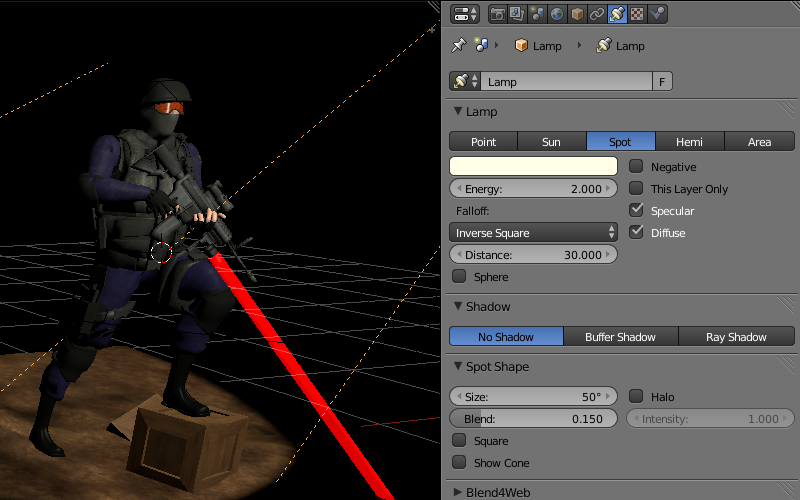
\includegraphics[width=1.000\linewidth]{lighting_setup.jpg}\hfill}

\begin{DUlineblock}{0em}
\item[] 
\end{DUlineblock}
\begin{description}
\item[{\emph{Color}}] \leavevmode
Цветовая характеристика света. Значение по умолчанию (1.0, 1.0, 1.0) (белый).

\item[{\emph{Energy}}] \leavevmode
Интенсивность излучения. Значение по умолчанию 1.0.

\item[{\emph{Falloff}}] \leavevmode
Тип затухания. Значение экспортируется, но в движке всегда используется \code{Inverse Square} (обратный квадратичный). Применяется для источников света типа \code{Point} и \code{Spot}. Значение по умолчанию \code{Inverse Square}.

\item[{\emph{Distance}}] \leavevmode
Параметр затухания. Применяется для источников света типа \code{Point} и \code{Spot}. Значение по умолчанию 25.0.

\item[{\emph{Spot Shape \textgreater{} Size}}] \leavevmode
Угол конуса в градусах. Применяется для источников света типа \code{Spot}. Значение по умолчанию 45º.

\item[{\emph{Spot Shape \textgreater{} Blend}}] \leavevmode
Параметр смягчения края светового пятна. Применяется для источников света типа \code{Spot}. Значение по умолчанию 0.15.

\item[{\emph{Blend4Web \textgreater{} Do not export}}] \leavevmode
Не экспортировать. По умолчанию отключено.

\item[{\emph{Blend4Web \textgreater{} Generate shadows}}] \leavevmode
Источник света используется для расчета падающих теней. Применяется в случае наличия нескольких источников света. По умолчанию отключено.

\item[{\emph{Blend4Web \textgreater{} Dynamic intesity}}] \leavevmode
Источник света используется для расчета изменения времени суток. Применяется для источников света типа ``Солнце''. По умолчанию отключено.

\end{description}


\section{Освещение от окружающей среды}
\label{lighting:id5}
Движком используется простая полусферическая модель освещения, в которой задается цвет горизонта и цвет зенита.


\subsection{Активация}
\label{lighting:id6}
Включить опцию \code{Environment Lighting} во вкладке \code{World}.

{\hfill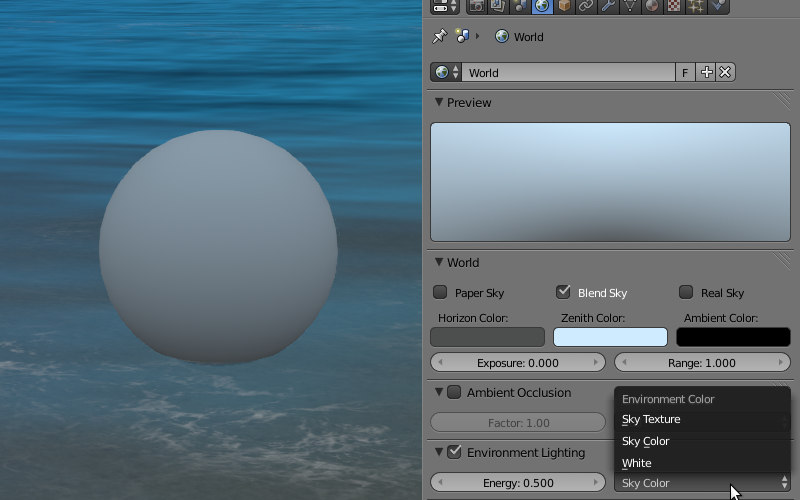
\includegraphics[width=1.000\linewidth]{lighting_environment.jpg}\hfill}


\subsection{Настройка}
\label{lighting:id7}\begin{description}
\item[{\emph{Environment Lighting \textgreater{} Energy}}] \leavevmode
Интенсивность освещения от окружающей среды. Значение по умолчанию 1.0.

\item[{\emph{Environment Lighting \textgreater{} Environment Color}}] \leavevmode
Тип источника освещения, поддерживаются \code{White} и \code{Sky Color}. При выборе \code{White} назначается белый цвет горизонта и белый цвет зенита. При выборе \code{Sky Color} цвет горизонта и цвет зенита задаются цветоподборщиками \code{World \textgreater{} Horizon Color} и \code{World \textgreater{} Zenith Color}. Значение по умолчанию \code{White}.

\item[{\emph{World \textgreater{} Horizon Color} и \emph{World \textgreater{} Zenith Color}}] \leavevmode
Цвет горизонта и цвет зенита. При выборе цвета рекомендуется активировать опцию \code{World \textgreater{} Blend Sky}.

\end{description}


\section{Тени}
\label{lighting:id8}

\subsection{Активация}
\label{lighting:id9}\begin{enumerate}
\item {} 
На объектах, \textbf{отбрасывающих} тени, включить опцию \code{Blend4Web \textgreater{} Shadows: Cast} во вкладке \code{Object}.

\item {} 
На объектах, \textbf{получающих} тени, включить опцию \code{Blend4Web \textgreater{} Shadows: Receive} во вкладке \code{Object}.

\item {} 
Убедиться, что включена опция \code{Blend4Web \textgreater{} Render shadows} во вкладке \code{Scene}.

\end{enumerate}


\subsection{Настройка}
\label{lighting:id10}\begin{description}
\item[{\emph{Направление}}] \leavevmode
В случае наличия нескольких источников света рекомендуется указать, какой именно источник света будет использоваться для расчета падающих теней, включив опцию \code{Blend4Web \textgreater{} Generate shadows} во вкладке \code{Object Data} при выборе объекта-лампы.

\item[{\emph{Цвет}}] \leavevmode
Цвет тени определяется настройками освещения от окружающей среды.

\end{description}

Во вкладке \code{World} на панели \code{Blend4Web \textgreater{} Shadow Settings} находятся дополнительные настройки:
\begin{description}
\item[{\emph{Optimize shadow volume}}] \leavevmode
Оптимизировать пространство для расчета теней. Если опция включена, производится движком производится оптимизация пространства для расчета теней под объем, занимаемый отбрасывающими тень объектами, что приводит к улучшению качества теней для локальных сцен. Если опция выключена, такая оптимизация не производится, что приводит к улучшению качества теней для протяженных сцен. По умолчанию включено.

\end{description}


\subsubsection{Каскады}
\label{lighting:id11}
Для обеспечения приемлемого качества теней и одновременно покрытия значительных пространств необходимо использовать несколько стадий генерации теней (каскадов). При этом вблизи наблюдателя располагается каскад с наилучшим качеством, вдали от наблюдателя — с наихудшим.

{\hfill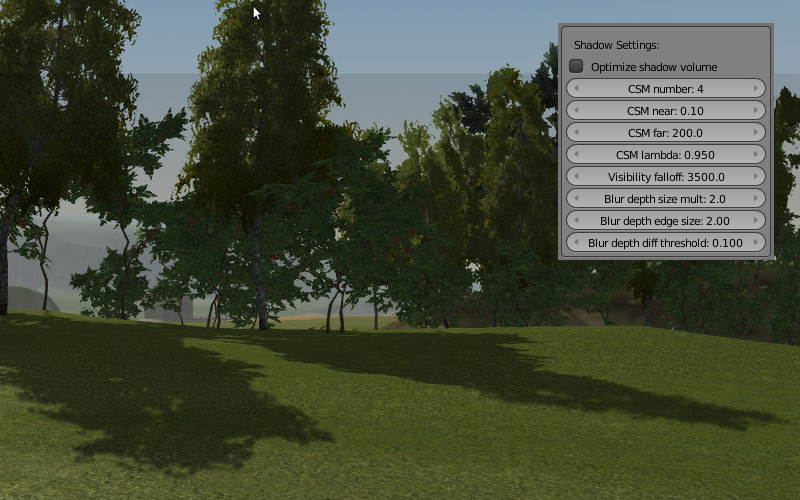
\includegraphics[width=1.000\linewidth]{shadow_cascades.jpg}\hfill}

\begin{DUlineblock}{0em}
\item[] 
\end{DUlineblock}
\begin{description}
\item[{\emph{CSM number}}] \leavevmode
Количество каскадов теней. Поддерживается от 1 до 4 каскадов. Значение по умолчанию 3.

\item[{\emph{CSM near}}] \leavevmode
Ближняя граница отображения теней. Значение по умолчанию 0.1.

\item[{\emph{CSM far}}] \leavevmode
Дальняя граница отображения теней. Значение по умолчанию 100.0.

\item[{\emph{CSM lambda}}] \leavevmode
Фактор распределения границ между каскадами. Рассчитанные значения границ каскадов отображаются в просмотрщике во вкладке \code{Shadows}. Значение по умолчанию 0.875.

\end{description}


\subsubsection{Мягкие тени}
\label{lighting:id12}\begin{description}
\item[{\emph{Visibility falloff}}] \leavevmode
Фактор экспонециального уменьшения видимости тени в зависимости от расстояния от точки отбрасывания до точки получения. Применяется для уменьшения видимости артефактов собственных теней (т.е. отбрасывания объектом тени на себя). Значение по умолчанию 3500.0.

\item[{\emph{Blur depth size mult}}] \leavevmode
Размер ядра сглаживания. Влияет на степень смягчения теней. Значение по умолчанию 1.0.

\item[{\emph{Blur depth edge size}}] \leavevmode
Разница между сэмплами (в текселях) при определении границ. Уменьшает ореол, исключая сглаживание границ. Значение по умолчанию 2.0.

\item[{\emph{Blur depth diff threshold}}] \leavevmode
Максимум разницы глубины при определении границ, умноженный на 1000. Уменьшает ореол, исключая сглаживание границ. Значение по умолчанию 0.1.

\end{description}


\chapter{Постпроцессинговые эффекты}
\label{postprocessing_effects:postprocessing-effects}\label{postprocessing_effects::doc}\label{postprocessing_effects:id1}
\index{размытие при движении}\index{motion blur}

\section{Размытие при движении}
\label{postprocessing_effects:id2}\label{postprocessing_effects:motion-blur}\label{postprocessing_effects:index-0}
Эффект размытия при движении (motion blur) служит целям увеличения реализма интерактивной сцены. Он проявляется при движении камеры или объектов в виде ``смазывания'' изображения.


\subsection{Активация}
\label{postprocessing_effects:id3}
Выставить опцию \code{Enable Motion Blur} на панели \code{Scene \textgreater{} Blend4Web}.


\subsection{Дополнительные настройки}
\label{postprocessing_effects:id4}
На панели \code{World \textgreater{} Blend4Web \textgreater{} Motion blur settings}:
\begin{description}
\item[{\emph{Motion blur factor}}] \leavevmode
Степень проявления эффекта. Чем выше значение, тем сильнее эффект размытие. Значение по умолчанию 0.01.

\item[{\emph{Motion blur decay threshold}}] \leavevmode
Степень плавности размытия. Чем выше значение, тем более резким будет эффект. Значение по умолчанию 0.01.

\end{description}

{\hfill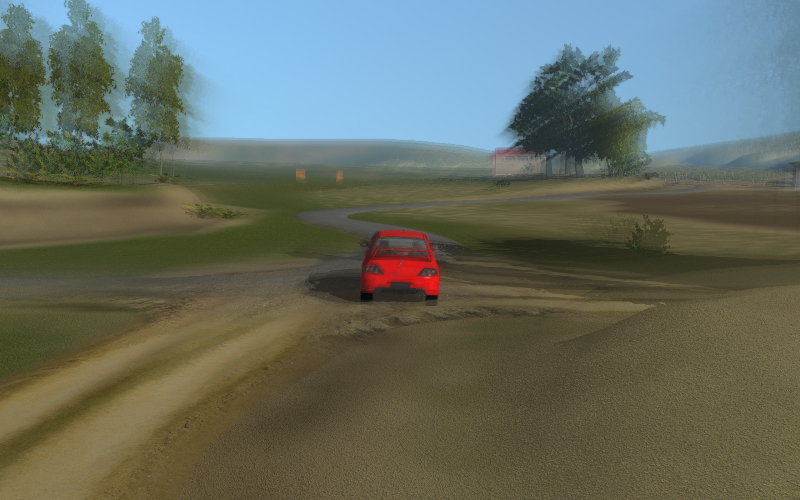
\includegraphics[width=1.000\linewidth]{motion_blur.jpg}\hfill}

\begin{DUlineblock}{0em}
\item[] 
\end{DUlineblock}

\index{глубина резкости камеры}\index{depth of field}\index{DOF}

\section{Глубина резкости камеры}
\label{postprocessing_effects:id5}\label{postprocessing_effects:dof}\label{postprocessing_effects:index-1}
Эффект глубины резкости камеры (depth of field, DOF) акцентирует внимание зрителя на части сцены. Проявляется в размытии изображения ближе и дальше от фокуса камеры.


\subsection{Активация}
\label{postprocessing_effects:id6}\begin{enumerate}
\item {} 
Выбрать активную камеру, перейти на панель ее настроек (\code{Object Data}).

\item {} 
Далее возможны два варианта:
\begin{itemize}
\item {} 
На панели \code{Depth of Field} в меню \code{Focus} выбрать объект, на котором будет сфокусирована камера. В этом случае при удалении или приближении к этому объекту будет происходит соответствующая коррекция фокуса камеры.

\item {} 
На панели \code{Depth of Field} установить ненулевое значение \code{Distance} (в метрах). В этом случае фокус камеры будет располагаться на заданном расстоянии от камеры и перемещаться вместе с ней.

\end{itemize}

\end{enumerate}


\subsection{Дополнительные настройки}
\label{postprocessing_effects:id7}
На панели настроек активной камеры \code{Object Data \textgreater{} Blend4Web}:
\begin{description}
\item[{\emph{DOF front distance}}] \leavevmode
Расстояние от фокуса до ближней к камере плоскости, за которой происходит полное размытие (в метрах). Значение по умолчанию 1.0.

\item[{\emph{DOF rear distance}}] \leavevmode
Расстояние от фокуса до дальней от камеры плоскости, за которой происходит полное размытие (в метрах). Значение по умолчанию 1.0.

\item[{\emph{DOF power}}] \leavevmode
Степень размытия. Значение по умолчанию 3.0.

\end{description}

{\hfill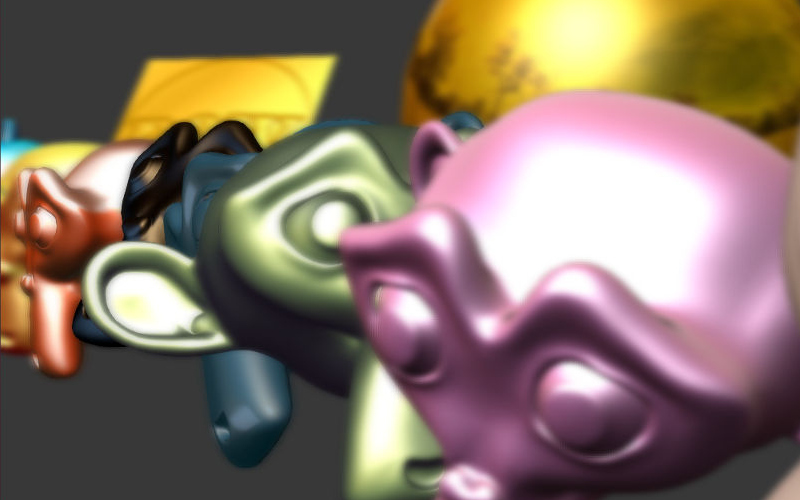
\includegraphics[width=1.000\linewidth]{dof.jpg}\hfill}

\begin{DUlineblock}{0em}
\item[] 
\end{DUlineblock}

\index{взаимное затенение}\index{screen-space ambient occlusion}\index{SSAO}

\section{Взаимное затенение}
\label{postprocessing_effects:index-2}\label{postprocessing_effects:ssao}\label{postprocessing_effects:id8}
Эффект взаимного затенения (screen-space ambient occlusion, SSAO) применяется с целью воспроизведения сложного переотражения света от объектов. Пространство между близкими объектами менее доступно для рассеянного света и поэтому затеняется сильнее.


\subsection{Активация}
\label{postprocessing_effects:id9}
Выставить опцию \code{Enable SSAO} на панели \code{Scene \textgreater{} Blend4Web}.


\subsection{Дополнительные настройки}
\label{postprocessing_effects:id10}
На панели ``мира'' \code{World \textgreater{} Blend4Web \textgreater{} SSAO Settings}:
\begin{description}
\item[{\emph{Radius Increase}}] \leavevmode
Фактор умножения радиуса сферического сэмплинга при переходе от внутреннего кольца к внешнему. Значение по умолчанию 1.7.

\item[{\emph{Dithering Amount}}] \leavevmode
Степень подмешивания случайного шума для уменьшения проявления полос (дитеринг). Значение по умолчанию 0.1.

\item[{\emph{Gauss Center}}] \leavevmode
Математическое ожидание - параметр распределения Гаусса для разницы глубин пиксела и соседнего сэмпла. Значение по умолчанию 0.2.

\item[{\emph{Gauss Width}}] \leavevmode
Стандартное отклонение - параметр распределения Гаусса для разницы глубин пиксела и соседнего сэмпла. Значение по умолчанию 2.0.

\item[{\emph{Gauss Width Left}}] \leavevmode
Стандартное отклонение в случае, когда разница глубин меньше математического ожидания. Значение по умолчанию 0.1.

\item[{\emph{Influence}}] \leavevmode
Степень проявленности эффекта взаимного затенения. Значение по умолчанию 0.7.

\item[{\emph{Distance Factor}}] \leavevmode
Фактор уменьшения проявленности эффекта взаимного затенения с расстоянием. Значение по умолчанию 0.0 (т.е. уменьшения нет).

\item[{\emph{Samples}}] \leavevmode
Количество сэмплов (чем больше, тем лучше качество, но меньше производительность). Значение по умолчанию 16.

\end{description}

{\hfill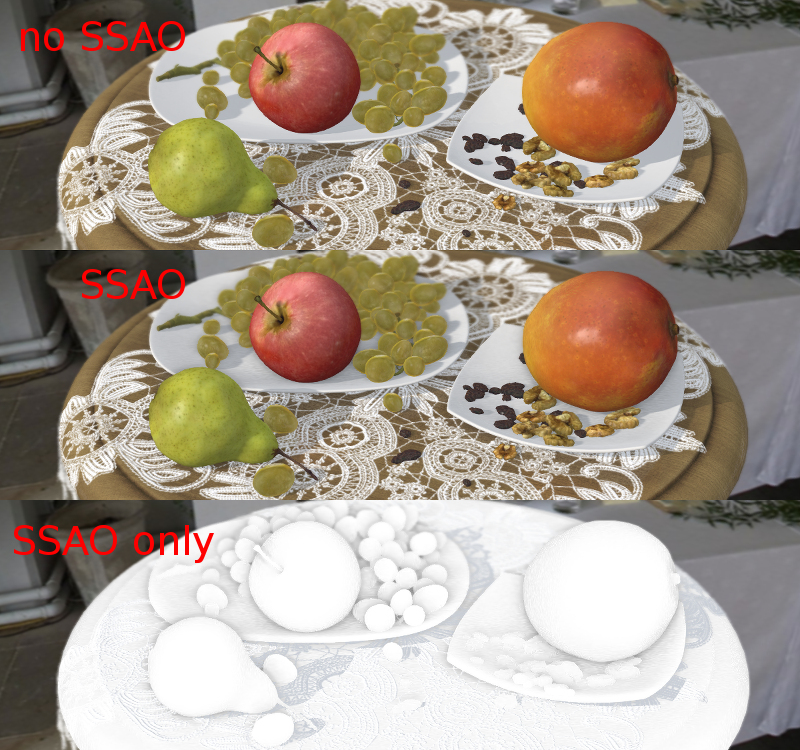
\includegraphics[width=1.000\linewidth]{ssao.jpg}\hfill}

\begin{DUlineblock}{0em}
\item[] 
\end{DUlineblock}

\index{сумеречные лучи}\index{crepuscular rays}\index{god rays}

\section{Сумеречные лучи}
\label{postprocessing_effects:god-rays}\label{postprocessing_effects:id11}\label{postprocessing_effects:index-3}
Эффект сумеречных лучей (crepuscular rays, ``god rays'') симулирует известное природное явление - свечение освещенных областей воздуха.


\subsection{Активация}
\label{postprocessing_effects:id12}
Выставить опцию \code{Enable God Rays} на панели \code{Scene \textgreater{} Blend4Web}.


\subsection{Дополнительные настройки}
\label{postprocessing_effects:id13}
На панели ``мира'' \code{World \textgreater{} Blend4Web \textgreater{} God Rays Settings}:
\begin{description}
\item[{\emph{God Rays Intencity}}] \leavevmode
Степень проявленности эффекта. Значение по умолчанию 0.7.

\item[{\emph{Maximum Ray Length}}] \leavevmode
Фактор длины лучей. Определяет шаг сэмплов радиального размытия. Значение по умолчанию 1.0.

\end{description}

{\hfill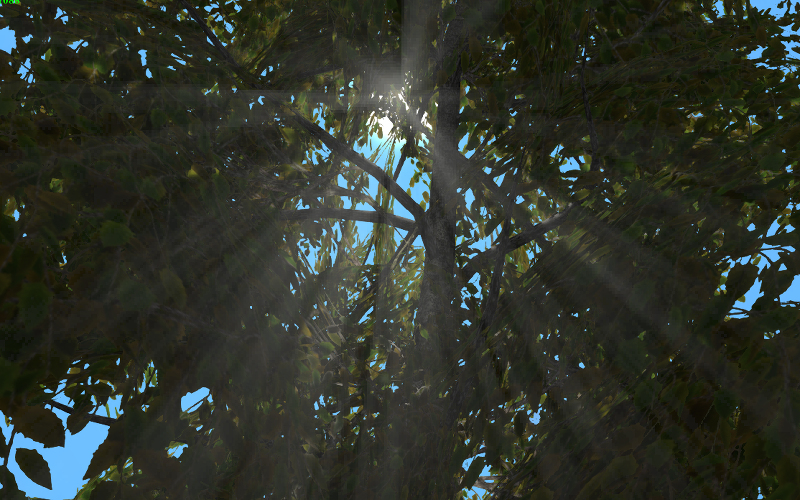
\includegraphics[width=1.000\linewidth]{god_rays.jpg}\hfill}

\begin{DUlineblock}{0em}
\item[] 
\end{DUlineblock}

\index{анаглиф}\index{стереоизображение}\index{anaglyph}

\section{Анаглиф стереоизображение}
\label{postprocessing_effects:anaglyph}\label{postprocessing_effects:index-4}\label{postprocessing_effects:id14}

\subsection{Активация}
\label{postprocessing_effects:id15}
Режим стереоизображения предназначен для просмотра контента в специальных очках и активируется приложением.


\subsection{Дополнительные настройки}
\label{postprocessing_effects:id16}
Нет.

{\hfill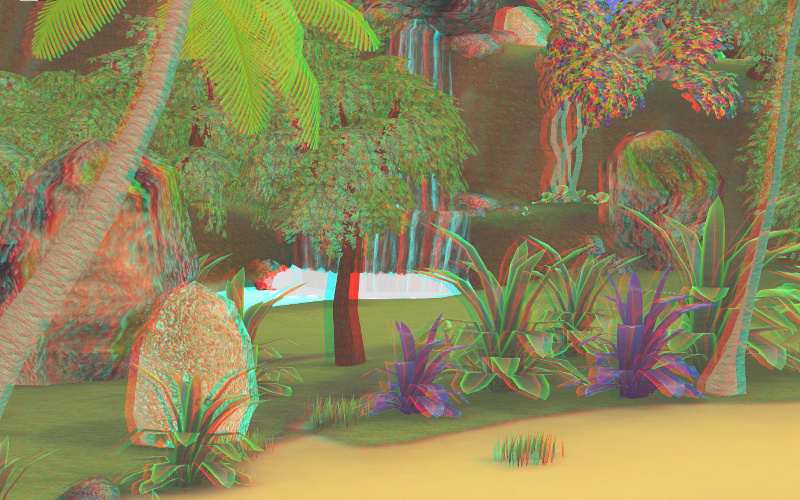
\includegraphics[width=1.000\linewidth]{anaglyph.jpg}\hfill}

\begin{DUlineblock}{0em}
\item[] 
\end{DUlineblock}

\index{коррекция цвета}\index{color correction}

\section{Коррекция цвета}
\label{postprocessing_effects:index-5}\label{postprocessing_effects:color-correction}\label{postprocessing_effects:id17}

\subsection{Активация}
\label{postprocessing_effects:id18}
Выставить опцию \code{Enable Color Correction} на панели \code{Scene \textgreater{} Blend4Web}.


\subsection{Дополнительные настройки}
\label{postprocessing_effects:id19}
На панели ``мира'' \code{World \textgreater{} Blend4Web \textgreater{} Color Correction Settings}:
\begin{description}
\item[{\emph{Brightness}}] \leavevmode
Яркость. Значение по умолчанию 0.0.

\item[{\emph{Contrast}}] \leavevmode
Контрастность. Значение по умолчанию 0.0.

\item[{\emph{Exposure}}] \leavevmode
Экспозиция. Значение по умолчанию 1.0.

\item[{\emph{Saturation}}] \leavevmode
Насыщенность. Значение по умолчанию 1.0.

\end{description}

{\hfill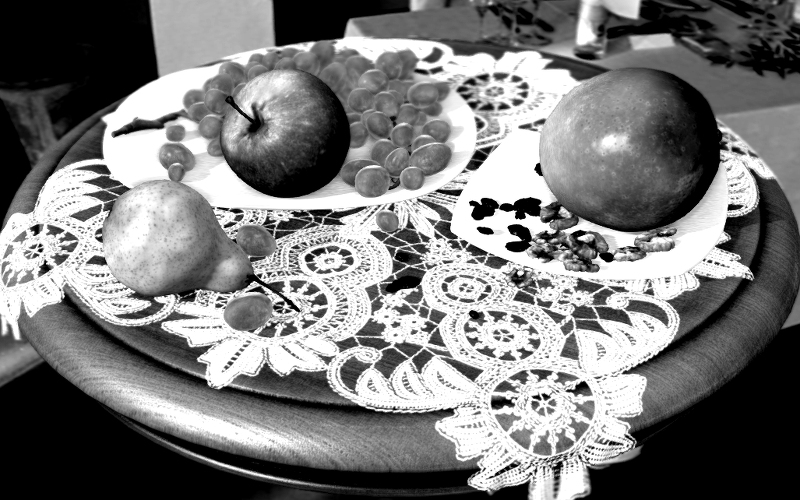
\includegraphics[width=1.000\linewidth]{color_correction.jpg}\hfill}

\begin{DUlineblock}{0em}
\item[] 
\end{DUlineblock}

\index{сглаживание}\index{anti-aliasing}

\section{Сглаживание}
\label{postprocessing_effects:antialiasing}\label{postprocessing_effects:id20}\label{postprocessing_effects:index-6}
Сглаживание (anti-aliasing) необходимо для уменьшения влияния нежелательных артефактов рендеринга (``зубчатости'').


\subsection{Активация}
\label{postprocessing_effects:id21}
Выставить опцию \code{Enable Antialiasing} на панели \code{Scene \textgreater{} Blend4Web}.


\subsection{Дополнительные настройки}
\label{postprocessing_effects:id22}
Приложение может выбрать выбрать режимы сглаживания: FXAA Quality (используется по умолчанию), FXAA ``Light'', или отключить сглаживание.

{\hfill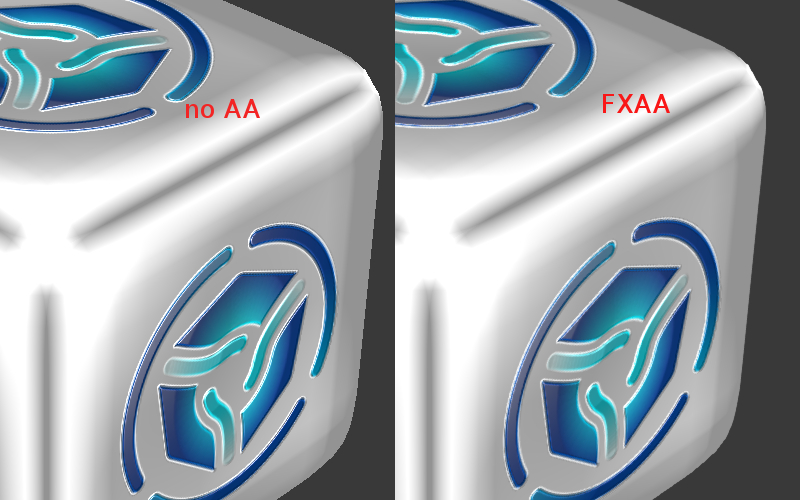
\includegraphics[width=1.000\linewidth]{antialiasing.jpg}\hfill}

\begin{DUlineblock}{0em}
\item[] 
\end{DUlineblock}


\section{Эффект засветки ярких деталей}
\label{postprocessing_effects:id23}
Эффект засветки (Bloom) проявляется при наличии на экране элементов с большой разницей в яркости. Вокруг ярких деталей создается светящийся ореол.


\subsection{Активация}
\label{postprocessing_effects:id24}
Выставить опцию \code{Enable Bloom} на панели \code{Scene \textgreater{} Blend4Web}.


\subsection{Дополнительные настройки}
\label{postprocessing_effects:id25}
На панели ``мира'' \code{World \textgreater{} Blend4Web \textgreater{} Bloom Settings}:
\begin{description}
\item[{\emph{Key}}] \leavevmode
Интенсивность эффекта свечения.

\item[{\emph{Blur}}] \leavevmode
Степень размытия засветки.

\item[{\emph{Edge Luminance}}] \leavevmode
Граничное значение относительной яркости элемента, выше которого начинает проявляться эффект засветки.

\end{description}

{\hfill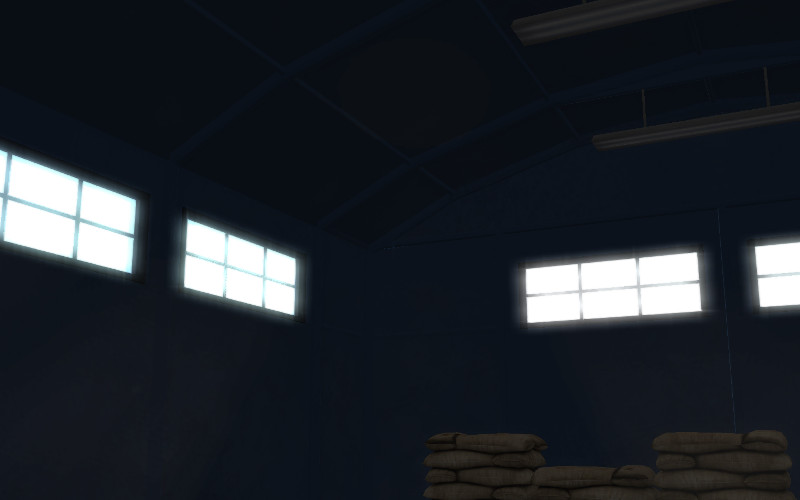
\includegraphics[width=1.000\linewidth]{bloom.jpg}\hfill}

\begin{DUlineblock}{0em}
\item[] 
\end{DUlineblock}

\index{свечение}\index{glow}

\section{Свечение вокруг объекта (Glow)}
\label{postprocessing_effects:id26}\label{postprocessing_effects:index-7}\label{postprocessing_effects:glow}
Эффект Glow заключается в подсвечивании конкретного объекта по контуру некоторым цветом. В результате вокруг объекта будет создан светящийся ореол.


\subsection{Активация}
\label{postprocessing_effects:id27}
Эффект Glow активируется программно через API. Может быть реализован как эффект постоянного свечения, так и затухающего, пульсирующего и любой другой модели. Чтобы разрешить его использование на конкретном объекте, необходимо выставить опцию \code{Selectable} на панели \code{Object \textgreater{} Blend4Web}.


\subsection{Дополнительные настройки}
\label{postprocessing_effects:id28}
На панели \code{Object \textgreater{} Blend4Web}:
\begin{description}
\item[{\emph{Glow duration}}] \leavevmode
Длительность Glow-анимации, сек. Значение по умолчанию 1.

\item[{\emph{Glow period}}] \leavevmode
Период повторения Glow-анимации, сек. Значение по умолчанию 1.

\item[{\emph{Glow relapses}}] \leavevmode
Количество итераций Glow-анимации. В случае 0 анимация будет повторяться бесконечно. Значение по умолчанию 0.

\end{description}

На панели \code{World \textgreater{} Blend4Web}:
\begin{description}
\item[{\emph{Objects glow color}}] \leavevmode
Общий цвет эффекта для всех объектов. Значение по умолчанию (0,0,0).

\item[{\emph{Glow factor}}] \leavevmode
Толщина и яркость ореола, окружающего объект. Падает с уменьшением параметра. Значение по умолчанию 1.

\end{description}

При управлении через API данные настройки воспринимаются как настройки по умолчанию.

{\hfill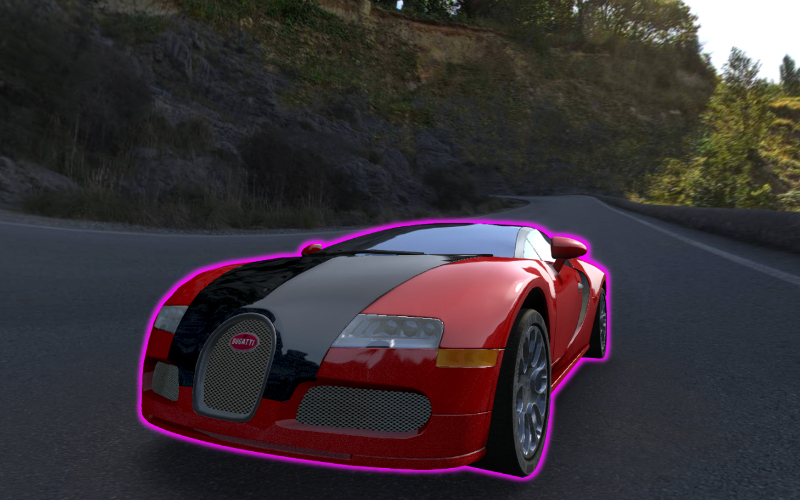
\includegraphics[width=1.000\linewidth]{glow.jpg}\hfill}
\phantomsection\label{particles:particles}
\index{система частиц}

\chapter{Система частиц}
\label{particles:index-0}\label{particles::doc}\label{particles:id1}
Система частиц предназначена для визуализации явлений, обусловленных движением множественных малых объектов, таких как дым, огонь, брызги воды и др.

{\hfill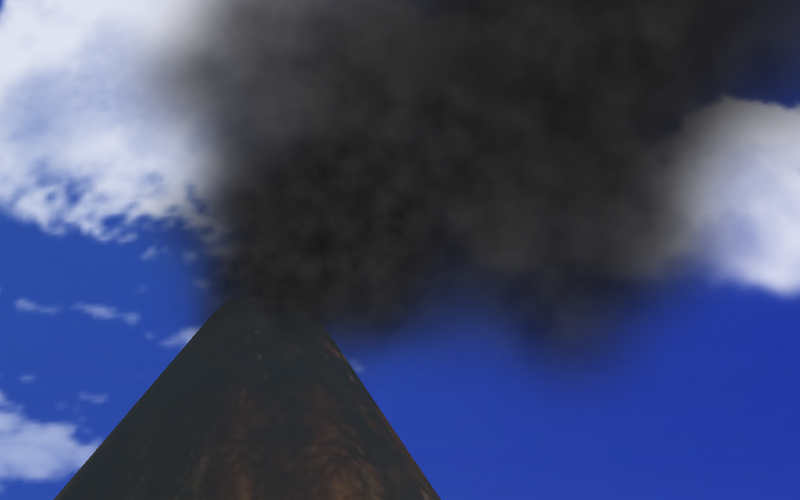
\includegraphics[width=1.000\linewidth]{particles_smoke.jpg}\hfill}

\begin{DUlineblock}{0em}
\item[] 
\end{DUlineblock}

Необходимым элементом системы частиц является эмиттер - объект, определяющий местоположение и направление исходящего потока частиц.


\section{Использование}
\label{particles:id2}

\subsection{Необходимые этапы}
\label{particles:id3}\begin{enumerate}
\item {} 
Добавить на сцену меш - эмиттер.

\item {} 
Создать на эмиттере материал для частиц, например типа \code{Halo}. Поддерживается также материал типа \code{Surface} с обязательной диффузной текстурой.

\item {} 
Добавить на эмиттере систему частиц.

\item {} \begin{description}
\item[{Инициализировать воспроизведение в движке. Возможны два варианта:}] \leavevmode\begin{itemize}
\item {} 
``циклическое испускание'' - для системы частиц выставить опцию \code{Blend4Web \textgreater{} Cyclic emission}.

\item {} 
``нециклическая анимация'' - для эмиттера выставить опцию \code{Blend4Web \textgreater{} Animation \textgreater{} Use default}.

\end{itemize}

\end{description}

\end{enumerate}


\subsection{Рекомендуемые дополнительные настройки}
\label{particles:id4}\begin{enumerate}
\item {} 
Для материала частиц выставить тип прозрачности \code{Add}.

\item {} 
Если отображение эмиттера на сцене не требуется, отключить опцию \code{Particles \textgreater{} Render \textgreater{} Emitter}.

\item {} 
Если отображение эмиттера на сцене необходимо, для него можно использовать дополнительные материалы. В этом случае в настройках системы частиц нужно указать номер материала частиц \code{Particles \textgreater{} Render \textgreater{} Material} (начиная с единицы).

\item {} 
В случае использования для частиц материала типа \code{Surface}, к материалу необходимо подключить диффузную текстуру (обычно с альфа-каналом). В меню \code{Mapping \textgreater{} Coordinates} выбрать \code{UV}.  Убедиться, что меш эмиттера имеет развертку.

\end{enumerate}

{\hfill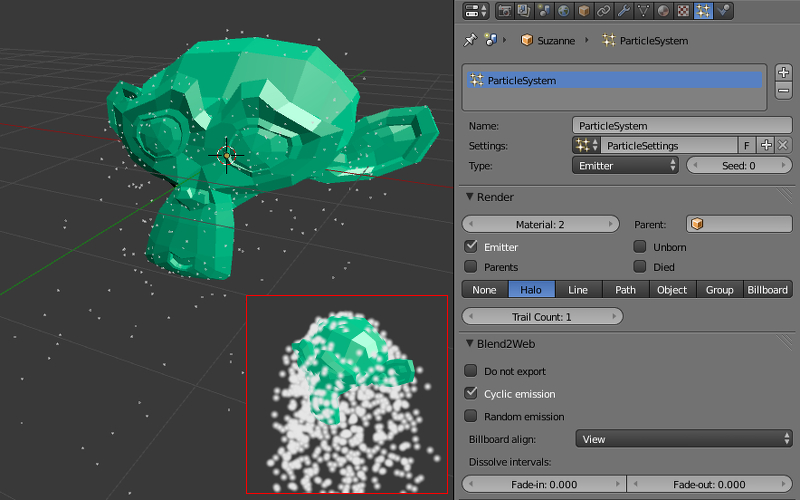
\includegraphics[width=1.000\linewidth]{particles_first_steps.jpg}\hfill}


\section{Настройка}
\label{particles:id5}
Параметры системы частиц настраиваются во вкладке \code{Particles}. Поддерживается несколько систем частиц на одном эмиттере.


\subsection{Общие настройки}
\label{particles:id6}\begin{description}
\item[{\emph{Name}}] \leavevmode
Название системы частиц. Значение по умолчанию ``ParticleSystem''.

\item[{\emph{Settings}}] \leavevmode
Ссылка на блок данных с настройками системы частиц. Блоки данных с настройками могут быть общими для разных систем частиц.

\item[{\emph{Type}}] \leavevmode
Тип системы частиц: \code{Emitter} или \code{Hair}. Системы частиц типа \code{Hair} используются для создания множественных копий (инстансинга) объектов. Значение по умолчанию \code{Emitter}.

\item[{\emph{Seed}}] \leavevmode
Индекс в таблице случайных чисел, используемых для генерации системы частиц. Значение по умолчанию 0.

\end{description}


\subsection{Настройки испускания}
\label{particles:id7}\begin{description}
\item[{\emph{Emission \textgreater{} Number}}] \leavevmode
Количество частиц. Значение по умолчанию 1000.

\item[{\emph{Emission \textgreater{} Start}}] \leavevmode
Первый кадр, после которого начинается испускание частиц. Значение по умолчанию 1.0.

\item[{\emph{Emission \textgreater{} End}}] \leavevmode
Последний кадр, после которого прекращается испускание частиц. Значение по умолчанию 200.0.

\item[{\emph{Emission \textgreater{} Lifetime}}] \leavevmode
Время жизни частиц в кадрах. Значение по умолчанию 50.0.

\item[{\emph{Emission \textgreater{} Lifetime \textgreater{} Random}}] \leavevmode
Фактор случайности для времени жизни. Значение по умолчанию 0.0.

\item[{\emph{Emission \textgreater{} Emit From}}] \leavevmode
Источник испускания. Поддерживаются вершины \code{Verts}, грани \code{Faces}. Значение по умолчанию \code{Faces}.

\item[{\emph{Emission \textgreater{} Emit From \textgreater{} Distribution}}] \leavevmode
Настройки распределения испускания: \code{Jittered}, \code{Random}, \code{Grid}. Игнорируются движком. Всегда используется случайное распределение (\code{Random}). Значение по умолчанию \code{Jittered}.

\end{description}

{\hfill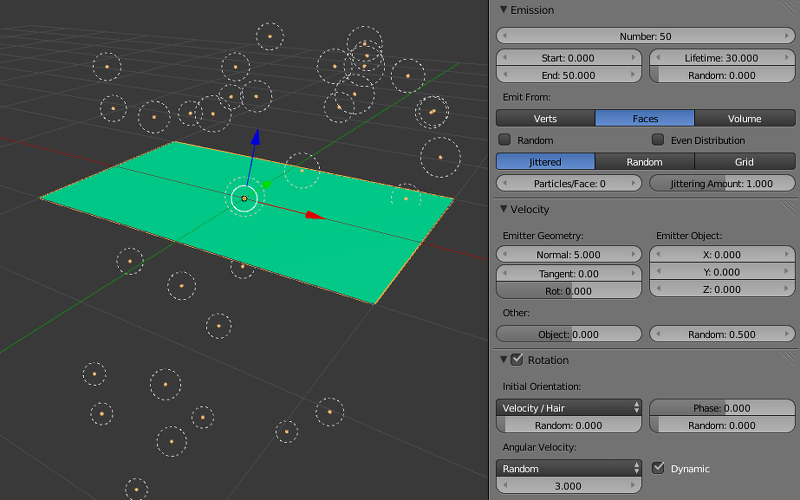
\includegraphics[width=1.000\linewidth]{particles_settings.jpg}\hfill}


\subsection{Настройки направления}
\label{particles:id8}
Поддерживаются только:
\begin{description}
\item[{\emph{Velocity \textgreater{} Emitter Geometry \textgreater{} Normal}}] \leavevmode
Фактор влияния на испускание вдоль нормалей меша эмиттера. Значение по умолчанию 1.0.

\item[{\emph{Velocity \textgreater{} Other \textgreater{} Random}}] \leavevmode
Фактор случайности для направления испускания. Значение по умолчанию 0.0.

\end{description}


\subsection{Настройки вращения}
\label{particles:id9}
Поддерживаются только:
\begin{description}
\item[{\emph{Rotation \textgreater{} Angular Velocity \textgreater{} Mode}}] \leavevmode
Режим собственного вращения биллбордов частиц. Поддерживаются \code{Velocity} (постоянная скорость вращения), \code{Random} (случайное вращение), \code{None} (нет вращения). Значение по умолчанию \code{Velocity}.

\item[{\emph{Rotation \textgreater{} Angular Velocity \textgreater{} Factor}}] \leavevmode
Фактор скорости собственного вращения биллбордов частиц. Значение по умолчанию 0.0.

\end{description}


\subsection{Настройки физики}
\label{particles:id10}
Поддерживаются только:
\begin{description}
\item[{\emph{Physics \textgreater{} Type}}] \leavevmode
Тип расчетов физики: \code{No}, \code{Newtonian}, \code{Keyed}, \code{Boids}, \code{Fluid}. Игнорируется движком. Всегда используется физика Ньютона (\code{Newtonian}). Значение по умолчанию \code{Newtonian}.

\item[{\emph{Physics \textgreater{} Size}}] \leavevmode
Размер частиц. Значение по умолчанию 0.05.

\item[{\emph{Physics \textgreater{} Mass}}] \leavevmode
Масса частиц. Влияет на взаимодействие с силовыми полями (в частности, с ветром). Значение по умолчанию 1.0.

\item[{\emph{Physics \textgreater{} Forces \textgreater{} Brownian}}] \leavevmode
Экспортируется, но не используется движком.

\end{description}

{\hfill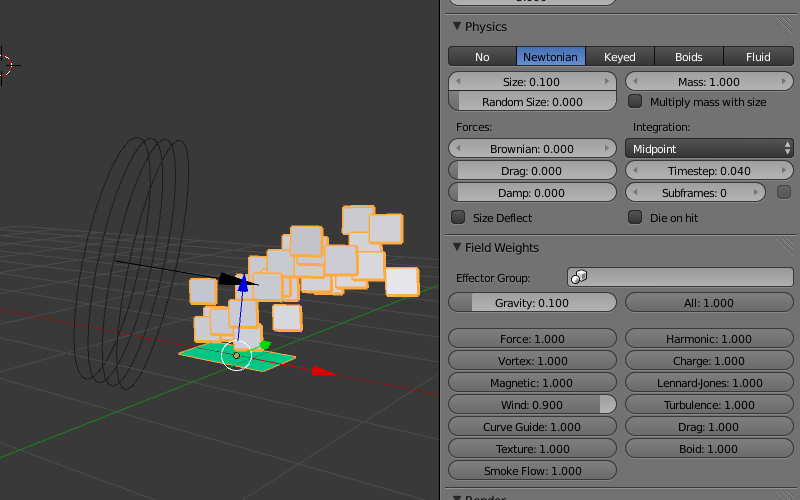
\includegraphics[width=1.000\linewidth]{particles_settings2.jpg}\hfill}


\subsection{Настройки отображения}
\label{particles:id11}
Поддерживаются только:
\begin{description}
\item[{\emph{Render \textgreater{} Material}}] \leavevmode
Номер материала частиц, начиная с единицы. Используется для указания на материал частиц в случае использования эмиттером нескольких материалов. Значение по умолчанию 1.

\item[{\emph{Render \textgreater{} Emitter}}] \leavevmode
Опция включения отображения эмиттера на сцене. По умолчанию включено.

\item[{\emph{Render \textgreater{} Type}}] \leavevmode
Режим отображения частиц: \code{None}, \code{Halo}, \code{Line}, \code{Path}, \code{Object}, \code{Group}, \code{Billboard}. Движком различаются режимы \code{Object} и \code{Group}, использующиеся для инстансинга объектов и групп объектов, соответственно. Другие режимы игнорируются. Для удобства отображения биллбордов рекомендуется включать режим \code{Billboard}. Значение по умолчанию \code{Halo}.

\end{description}


\subsection{Настройки влияния силовых полей}
\label{particles:id12}\label{particles:particles-force-fields}
Поддерживаются только:
\begin{description}
\item[{\emph{Field Weights \textgreater{} Gravity}}] \leavevmode
Фактор влияния гравитационного поля (земное притяжение). Значение по умолчанию 1.0.

\item[{\emph{Field Weights \textgreater{} Wind}}] \leavevmode
Фактор влияния ветра. Необходимо присутствие объекта силового поля (добавляется \code{Add \textgreater{} Force Field}) типа \code{Wind} (ветер). На систему частиц оказывают также настройки направления и силы ветра. Значение по умолчанию 1.0.

\end{description}


\subsection{Специальные настройки движка}
\label{particles:id13}\begin{description}
\item[{\emph{Blend4Web \textgreater{} Do not export}}] \leavevmode
Не поддерживается.

\item[{\emph{Blend4Web \textgreater{} Cyclic emission}}] \leavevmode
Опция включает циклический режим испускания. Применяется для постоянных эффектов (дым, горение, брызги). Рекомендуется выставить нулевое значение \code{Emission \textgreater{} Start}. По умолчанию выключено.

\item[{\emph{Blend4Web \textgreater{} Random emission}}] \leavevmode
Опция устанавливает случайный характер времени испускания частиц. По умолчанию выключено.

\item[{\emph{Blend4Web \textgreater{} Billboard align}}] \leavevmode
Способ ориентирования биллбордов: \code{View} - поворачивать к камере, \code{XY plane}, \code{YZ plane}, \code{ZX plane} - ориентировать в соответствующей плоскости (в мировой системе координат Blender'a). Значение по умолчанию \code{View}.

\item[{\emph{Blend4Web \textgreater{} Dissolve intervals \textgreater{} Fade-in} и \emph{Fade-out}}] \leavevmode
Начальный и конечный интервалы (в кадрах) для постепенного увеличения и уменьшения прозрачности частиц.

\end{description}


\section{Текстуры в системах частиц}
\label{particles:id14}\label{particles:particles-textures}

\subsection{Текстуры материала частиц}
\label{particles:id15}
В материалах частиц типа \code{Surface} \textbf{необходимо} наличие диффузной текстуры (обычно с альфа-каналом). В меню \code{Mapping \textgreater{} Coordinates} выбрать \code{UV}.  Убедиться, что меш эмиттера имеет развертку.

В материалах частиц типа \code{Halo} \textbf{возможно} использование текстуры типа \code{Blend} с линейным (\code{Linear}) градиентом. В меню \code{Mapping \textgreater{} Coordinates} выбрать \code{Strand / Particle}. На текстуре необходимо включить использование рампы (\code{Ramp}). Допускается использование до 4 контрольных точек градиента.

{\hfill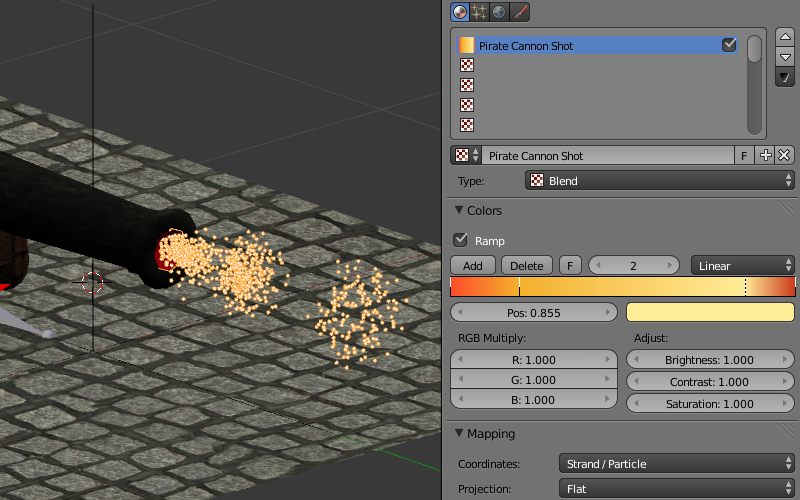
\includegraphics[width=1.000\linewidth]{particles_settings_ramp_color.jpg}\hfill}


\subsection{Текстуры системы частиц}
\label{particles:id16}
Для настройки поведения системы частиц могут быть использованы текстуры. В отличие от текстур, используемых материалами частиц, такие текстуры относятся к блоку данных (datablock) системы частиц, а не к блоку данных материала. Чтобы создать текстуру системы частиц, необходимо \textbf{из вкладки} \code{Particles} перейти во вкладку \code{Textures}, после чего нажать \code{New}.

Поддерживаются только текстуры типа \code{Blend} с линейным (\code{Linear}) градиентом. На текстуре необходимо включить использование рампы (\code{Ramp}). Допускается использование до 4 контрольных точек градиента.

На панели \code{Influence} необходимо выбрать параметр, на который воздействует текстура. В настоящий момент поддерживается только \code{Size} (размер).

{\hfill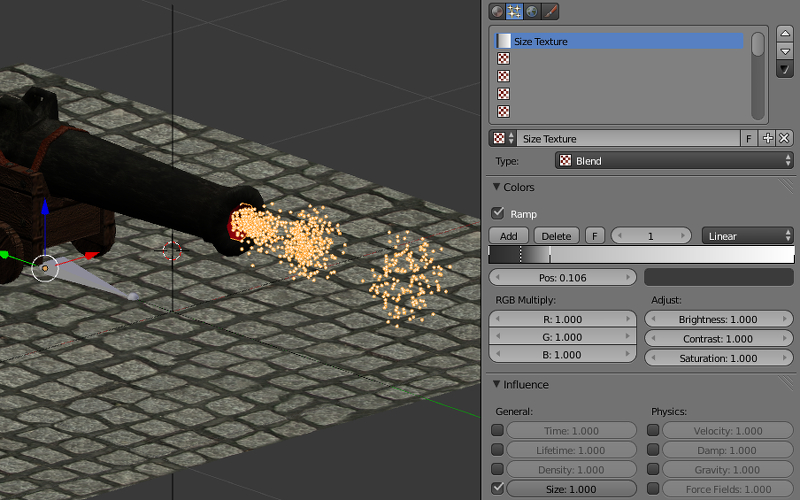
\includegraphics[width=1.000\linewidth]{particles_settings_ramp_size.jpg}\hfill}

\begin{DUlineblock}{0em}
\item[] 
\end{DUlineblock}

Результат применения текстур градиента для материала частиц и для системы частиц:

{\hfill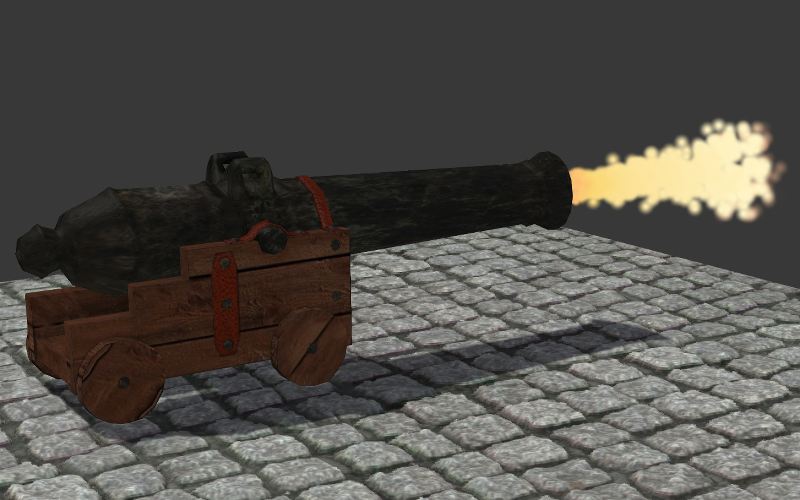
\includegraphics[width=1.000\linewidth]{particles_gun.jpg}\hfill}
\phantomsection\label{particles_instancing:particles-instancing}
\index{система частиц}\index{инстансинг}\index{instancing}

\chapter{Система частиц для инстансинга объектов}
\label{particles_instancing:index-0}\label{particles_instancing::doc}\label{particles_instancing:id1}
Система частиц может использоваться для создания множественных копий объектов (инстансинга).

{\hfill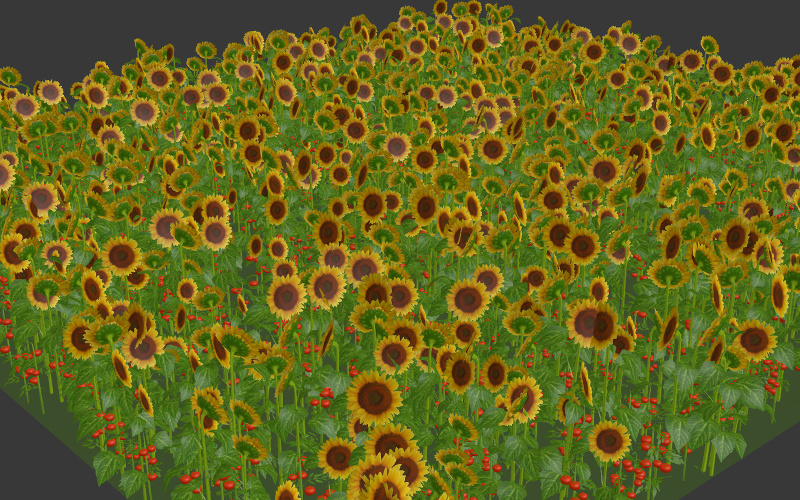
\includegraphics[width=1.000\linewidth]{particles_instancing_example.jpg}\hfill}


\section{Настройки системы частиц}
\label{particles_instancing:id2}
\textbf{Активация}
\begin{enumerate}
\item {} 
На эмиттере создать систему частиц типа \code{Hair}.

\item {} 
В панели \code{Render} выбрать тип отображения \code{Object} (или \code{Group}).

\item {} 
В поле \code{Dupli Object} (или \code{Dupli Group}) выбрать объект (или группу объектов) для инстансинга. Поддерживаются как локальные, так и подключенные по ссылке объекты (или группы).

\end{enumerate}

\textbf{Рекомендуемые дополнительные настройки}
\begin{enumerate}
\item {} 
Для корректного отображения размера установить значение 1.0 для параметров \code{Emission \textgreater{} Hair Length} и \code{Render \textgreater{} Size}.

\item {} 
Для установки корректной ориентации временно включить опцию \code{Advanced}, активировать панель \code{Rotation} и в меню \code{Initial Orientation} выбрать \code{None}. Отключить опцию \code{Advanced}. Также рекомендуется включить опцию \code{Render \textgreater{} Rotation}.

\end{enumerate}

{\hfill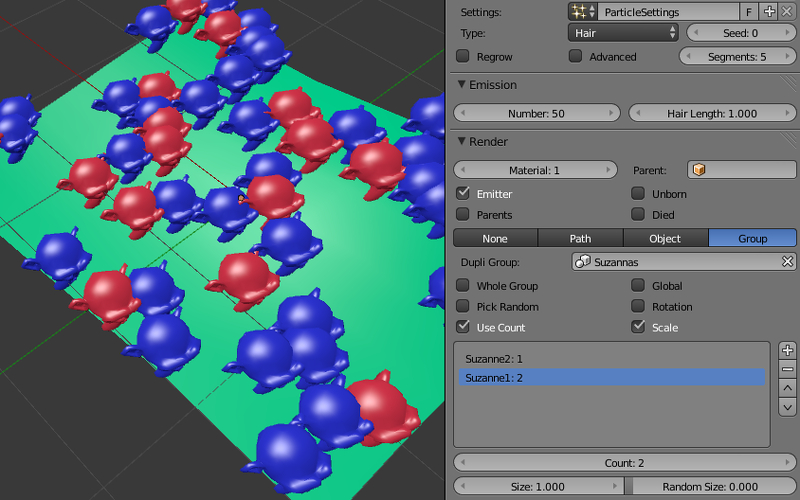
\includegraphics[width=1.000\linewidth]{particles_instancing_setup.jpg}\hfill}

\begin{DUlineblock}{0em}
\item[] 
\end{DUlineblock}

\textbf{Настройка}
\begin{description}
\item[{\emph{Render \textgreater{} Use Count}}] \leavevmode
Опция доступна для групп объектов-частиц. При включении появляется интерфейс установки относительного количества входящих в группу объектов. Движок не воспроизводит точное местонахождение объектов заданных типов.

\item[{\emph{Blend4Web \textgreater{} Random location and size}}] \leavevmode
Опция устанавливает случайный характер расположения и размеров объектов. Если опция включена, движок генерирует случайные координаты и размер (в пределах \(\pm\)25\%) объектов-частиц. Если опция выключена, производится экспорт и использование текущих координат и размеров объектов-частиц. По умолчанию включено.

\item[{\emph{Blend4Web \textgreater{} Initial random rotation}}] \leavevmode
Опция устанавливает случайный характер вращения объектов относительно оси определяемой параметром \code{Rotation type}. Если опция включена, движок генерирует случайные углы вращения объектов-частиц. Если опция выключена, устанавливается нулевой угол вращения. По умолчанию включено.

\item[{\emph{Blend4Web \textgreater{} Rotation type}}] \leavevmode\begin{description}
\item[{Ось случайного поворота объекта (опция доступна при включении \code{Blend4Web \textgreater{} Initial random rotation}). Возможны 2 варианта:}] \leavevmode\begin{itemize}
\item {} 
\code{Z axis} - случайный поворот будет осуществлен относительно вертикальной оси Z

\item {} 
\code{Random axis} - случайный поворот будет осуществлен относительно случайной оси

\end{itemize}

\end{description}

Значение по умолчанию \code{Z axis}.

\item[{\emph{Blend4Web \textgreater{} Rotation strength}}] \leavevmode\begin{description}
\item[{Коэффициент, определяющий диапазон случайных углов поворота, отсчитываемых от направления на камеру (опция доступна при включении \code{Blend4Web \textgreater{} Initial random rotation}). Например:}] \leavevmode\begin{itemize}
\item {} 
\code{Rotation strength = 1} - углы будут лежать в пределах \([-\pi, \pi]\)

\item {} 
\code{Rotation strength = 0.5} - углы будут лежать в пределах \([-0.5 \cdot \pi, 0.5 \cdot \pi]\)

\item {} 
\code{Rotation strength = 0.1} - углы будут лежать в пределах \([-0.1 \cdot \pi, 0.1 \cdot \pi]\)

\end{itemize}

\end{description}

Значение по умолчанию 1.

\item[{\emph{Blend4Web \textgreater{} Billboard}}] \leavevmode
Включение биллбординга для частиц. По умолчанию выключено.

\item[{\emph{Blend4Web \textgreater{} Billboard type}}] \leavevmode\begin{description}
\item[{Тип биллбординга (опция доступна при включении \code{Blend4Web \textgreater{} Billboard}). Доступны 3 типа:}] \leavevmode\begin{itemize}
\item {} 
\code{Basic} - простой односторонний биллбординг: частицы всегда будут повернуты лицевой стороной

\item {} 
\code{Random} - случайный двусторонний биллбординг: частицы чаще всего будут повернуты лицевой, либо обратной стороной, реже - боком; присутствует небольшой случайный поворот; модель создана специально для инстансинга травы

\item {} 
\code{Jittered} - односторонний биллбординг с колебанием частиц в плоскости, обращенной к наблюдателю; модель создана специально для инстансинга листвы деревьев

\end{itemize}

\end{description}

Значение по умолчанию \code{Basic}.

\item[{\emph{Blend4Web \textgreater{} Jitter amplitude}}] \leavevmode
Коэффициент амплитуды колебаний частиц (опция доступна при выборе типа \code{Jittered} в  \code{Blend4Web \textgreater{} Billboard type}). При увеличении параметра амплитуда растет. Значение по умолчанию 0.

\item[{\emph{Blend4Web \textgreater{} Jitter frequency}}] \leavevmode
Частота колебаний частиц, Гц (опция доступна при выборе типа \code{Jittered} в  \code{Blend4Web \textgreater{} Billboard type}). Значение по умолчанию 0.

\item[{\emph{Blend4Web \textgreater{} Billboard geometry}}] \leavevmode\begin{description}
\item[{Тип вращения биллбордов (опция доступна при включении \code{Blend4Web \textgreater{} Billboard}). Доступны 2 типа:}] \leavevmode\begin{itemize}
\item {} 
\code{Spherical} - сферический биллбординг, полная ориентация частиц по отношению к наблюдателю, вращение ничем не ограничено

\item {} 
\code{Cylindrical} - цилиндрический биллбординг, вращение частиц только относительно оси Z

\end{itemize}

\end{description}

Значение по умолчанию \code{Spherical}.

\item[{\emph{Blend4Web \textgreater{} Dynamic Grass}}] \leavevmode
Опция включает режим динамического рендеринга травяного покрова. По умолчанию отключено.

\item[{\emph{Blend4Web \textgreater{} Wind bending}}] \leavevmode\begin{description}
\item[{Наследование частицами настроек Wind bending:}] \leavevmode\begin{itemize}
\item {} 
\code{Parent} - наследование с эмиттера

\item {} 
\code{Instance} - наследование с объекта самой частицы

\end{itemize}

\end{description}

Значение по умолчанию \code{Parent}.

\item[{\emph{Blend4Web \textgreater{} Shadows}}] \leavevmode\begin{description}
\item[{Наследование частицами настроек теней:}] \leavevmode\begin{itemize}
\item {} 
\code{Parent} - наследование с эмиттера

\item {} 
\code{Instance} - наследование с объекта самой частицы

\end{itemize}

\end{description}

Значение по умолчанию \code{Parent}.

\item[{\emph{Blend4Web \textgreater{} Reflection}}] \leavevmode\begin{description}
\item[{Наследование частицами настроек отражений:}] \leavevmode\begin{itemize}
\item {} 
\code{Parent} - наследование с эмиттера

\item {} 
\code{Instance} - наследование с объекта самой частицы

\end{itemize}

\end{description}

Значение по умолчанию \code{Parent}.

\item[{\emph{Blend4Web \textgreater{} Vertex color}}] \leavevmode\begin{description}
\item[{Наследование частицами вертексного цвета с эмиттера. Содержит 2 поля:}] \leavevmode\begin{itemize}
\item {} 
\code{from} - имя существующего у эмиттера вертексного цвета

\item {} 
\code{to} - имя существующего у частицы вертексного цвета

\end{itemize}

\end{description}

По умолчанию наследования не происходит.

\end{description}


\section{Травяной покров}
\label{particles_instancing:id3}\label{particles_instancing:particles-grass}
Инстансинг объектов может использоваться для визуализации травяного покрова на обширных площадях. При этом происходит отрисовка травы вблизи камеры по мере ее движения по ландшафту.

{\hfill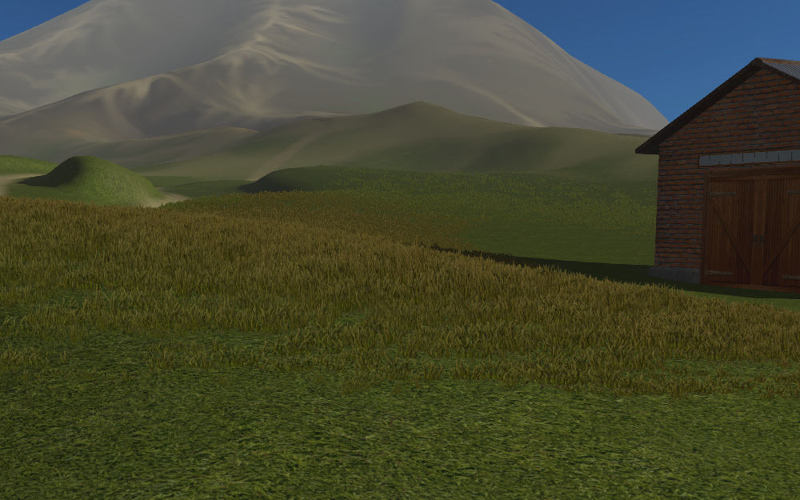
\includegraphics[width=1.000\linewidth]{dynamic_grass.jpg}\hfill}

\begin{DUlineblock}{0em}
\item[] 
\end{DUlineblock}

\textbf{Активация}
\begin{enumerate}
\item {} 
На отдельном объекте-плоскости создать систему частиц для инстансинга объектов. Включить опцию \code{Blend4Web \textgreater{} Dynamic Grass}.

\item {} 
На предполагаемом материале ландшафта включить опцию \code{Blend4Web \textgreater{} Terrain dynamic grass}.

\end{enumerate}

\textbf{Настройка}

Рекомендуется создать несколько плоскостей (например, 3) с размерами, соответствующими желаемому размеру каскада травяного покрова (например, 100, 150 и 250 м).

На \textbf{материале} ландшафта при включении опции \code{Blend4Web \textgreater{} Terrain dynamic grass} становятся активными текстовые поля:
\begin{description}
\item[{\emph{Dynamic grass size (R)}}] \leavevmode
Название слоя вертексного цвета меша ландшафта, предназначенного для модифицирования размера травяного покрова. Размер (``высота'') травяного покрова задается оттенками серого - чем светлее, тем больше.

\item[{\emph{Dynamic grass color (RGB)}}] \leavevmode
Название слоя вертексного цвета меша ландшафта, предназначенного для подкраски травяного покрова. Вертексный цвет умножается на цвет материала травы. Параметр \code{Influence \textgreater{} Blend} диффузной текстуры материала травы должен иметь значение \code{Multiply}.

\end{description}

Слои вертексного цвета с такими названиями должны существовать в меше ландшафта.

Рекомендуется также отключить отображение эмиттера (опция \code{Render \textgreater{} Emitter}).

{\hfill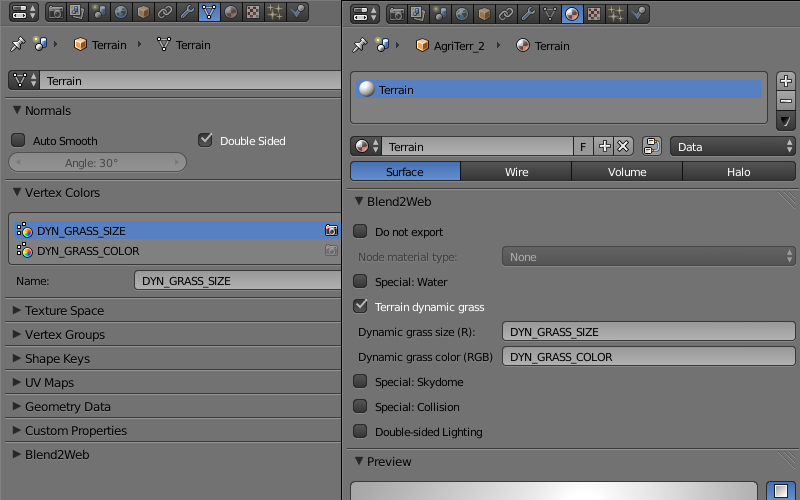
\includegraphics[width=1.000\linewidth]{dynamic_grass_setup.jpg}\hfill}


\section{Листва деревьев}
\label{particles_instancing:particles-leaves}\label{particles_instancing:id4}
Инстансинг хорошо подходит для отображения листвы на деревьях, и позволяет добиться более высокого уровня детализации.

{\hfill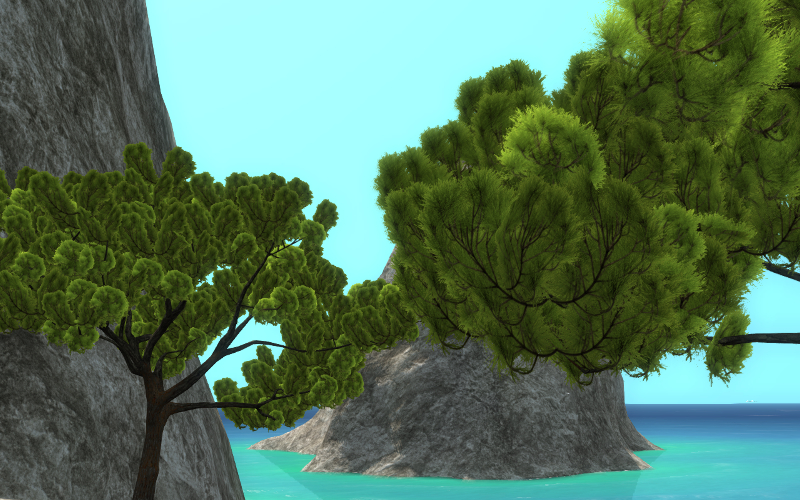
\includegraphics[width=1.000\linewidth]{tree_leaves.jpg}\hfill}

\begin{DUlineblock}{0em}
\item[] 
\end{DUlineblock}

\textbf{Активация}

Осуществляется как описано выше в разделе \code{Настройки системы частиц -\textgreater{} Активация}. Здесь соответственно эмиттером будет выступать дерево, а частицами - ветки, листья и т.д.

Для эмиттера дополнительно можно сделать следующее:
\begin{itemize}
\item {} 
создать вертексную группу, включающую вершины, на которых будут располагаться частицы

\item {} 
создать слой вертексного цвета для настройки Wind Bending дерева и листвы

\item {} 
создать слой вертексного цвета для наследования его частицами (можно использовать, например, для подкраски частиц)

\end{itemize}

\textbf{Настройка}
\begin{enumerate}
\item {} 
\code{Настройки случайного поворота}

\end{enumerate}

Если включена опция \code{Blend4Web \textgreater{} Initial random rotation}, то рекомендуется выставить вертикальную ось случайного поворота - \code{Z axis} (опция \code{Blend4Web \textgreater{} Rotation type}). Опция \code{Blend4Web \textgreater{} Rotation strength} - на свое усмотрение.
\begin{enumerate}
\setcounter{enumi}{1}
\item {} 
\code{Настройки биллбординга}

\end{enumerate}

Рекомендуется включить биллбординг, выставить тип \code{Jittered} (опция \code{Blend4Web \textgreater{} Billboard type}) и сделать его сферическим - \code{Spherical} (опция \code{Blend4Web \textgreater{} Billboard geometry}). Настройки \code{Blend4Web \textgreater{} Jitter amplitude} и \code{Blend4Web \textgreater{} Jitter frequency} - на свое усмотрение.
\begin{enumerate}
\setcounter{enumi}{2}
\item {} 
\code{Настройки расположения частиц}

\end{enumerate}

Рекомендуется выставить опцию \code{Emission \textgreater{} Emit From} в значение \code{Verts}, а в \code{Vertex Group \textgreater{} Density} выбрать вертексную группу эмиттера с вершинами для расположения частиц. Также нужно отключить опцию \code{Blend4Web \textgreater{} Random location and size}.
\begin{enumerate}
\setcounter{enumi}{3}
\item {} 
\code{Настройки Wind Bending}

\end{enumerate}

Рекомендуется включить наследование настроек из эмиттера - выставить \code{Parent} в опции \code{Blend4Web \textgreater{} Wind bending}. Затем у эмиттера в панели \code{Object} выбрать опцию \code{Blend4Web \textgreater{} Wind bending} и настроить параметры бендинга. Для дерева достаточно указать параметры \code{Blend4Web \textgreater{} Main Bending \textgreater{} Angle} и \code{Blend4Web \textgreater{} Main Bending \textgreater{} Frequency}, а также вертексный цвет для бендинга - \code{Blend4Web \textgreater{} Main Bending \textgreater{} Main stiffness}.
\begin{enumerate}
\setcounter{enumi}{4}
\item {} 
\code{Настройки наследования вертексного цвета}

\end{enumerate}

Для наследования частицами вертексного цвета эмиттера нужно указать имя цвета эмиттера и имя цвета частицы соответственно в полях \code{Blend4Web \textgreater{} Vertex Color \textgreater{} from} и \code{Blend4Web \textgreater{} Vertex Color \textgreater{} to}. При наследовании цвет ближайшей к частице вершины эмиттера из \code{from} будет скопирован и размножен в цвет \code{to} частицы.

Полученный таким образом вертексный цвет с именем \code{Blend4Web \textgreater{} Vertex Color \textgreater{} to} можно будет использовать в нодовом материале частицы для ее подкрашивания либо каких-то других эффектов.

{\hfill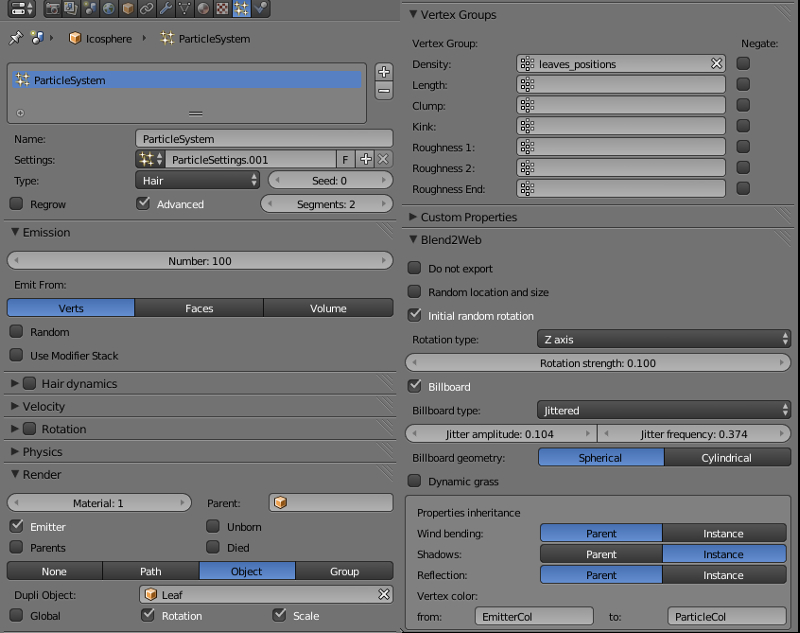
\includegraphics[width=1.000\linewidth]{particle_settings.jpg}\hfill}
\phantomsection\label{animation:animation}
\index{анимация}\index{animation}

\chapter{Анимация}
\label{animation:index-0}\label{animation::doc}\label{animation:id1}
В общем случае, к анимации относятся изменения параметров объектов во времени.
Движком поддерживаются следующие типы анимации:
\begin{itemize}
\item {} 
Перемещение объекта в пространстве как единого целого (объектная анимация).
Изменяемые параметры: координаты центра (\code{Location}), кватернион поворота
(\code{Rotation} в режиме \code{Quaternion(WXYZ)}) и масштабирование (\code{Scaling}).

\item {} 
Деформация объекта с помощью системы костей (скиннинг и скелетная анимация) а
также анимация костей в арматурном объекте для вспомогательных целей.

\item {} 
Покадровая запись деформаций объекта с последующим воспроизведением
(вертексная анимация).

\item {} 
Параметризация параметров источников звука. Изменяемые параметры: громкость
(\code{Volume}) и высота звука (\code{Pitch}).

\item {} 
Процедурная анимация в виде колебаний объекта под действием ветра. Описано
{\hyperref[outdoor_rendering:wind]{\emph{отдельно}}}.

\item {} 
Эмиссия частиц из источника. Описано в {\hyperref[particles:particles]{\emph{соответствующем разделе}}}.

\end{itemize}


\section{Управление анимацией}
\label{animation:id2}
Управление анимацией в движке осуществляется одним из трёх способов:
\begin{enumerate}
\item {} 
Автоматически, с помощью указания свойств \code{Animation: Use default} и
\code{Animation: Cyclic} в свойствах объекта. В данном случае будет осуществлён
поиск доступного метода и в случае положительного результата, объект
анимируется с момента загрузки сцены.

\item {} 
Программно, используя функции модуля \code{animation}.

\item {} 
Автоматически, с помощью редактирования файла \code{assets.json}. В настройках
загрузки сцены добавляется свойство \code{animated\_objects}, являющееся массивом
имён объектов, либо пар {[}''имя объекта-дупликатора группы'', ``имя объекта
внутри группы''{]}. Метод подходит только для приложений, использующих
информацию из файла \code{assets.json} (в настоящий момент к ним относится
просмоторщик сцен \code{viewer}).

\end{enumerate}

В случае анимации меша, необходимо назначение свойства \code{Do not batch} на
вкладке свойств объекта.


\section{Объектная анимация}
\label{animation:id3}
Осуществляется с помощью добавления ключей анимации в программе Blender и
их последующего воспроизведения в движке.

Поддерживаются следующие типы ключей:
\begin{itemize}
\item {} 
\emph{Location}

\item {} 
\emph{Rotation} -- необходимо осуществлять в режиме \code{Quaternion(WXYZ)}.

\item {} 
\emph{Scaling} -- для получения корректных результатов, фактор масштабирования должен быть одинаковым вдоль любых из осей.

\item {} 
\emph{LocRot} -- комбинация \emph{Location} и \emph{Rotation}.

\item {} 
\emph{LocScale} -- комбинация \emph{Location} и \emph{Scale}.

\item {} 
\emph{LocRotScale} -- комбинация \emph{Location}, \emph{Rotation} и \emph{Scale}.

\item {} 
\emph{RotScale} -- комбинация \emph{Rotation} и \emph{Scale}.

\end{itemize}


\section{Скиннинг и скелетная анимация}
\label{animation:id4}
Для осуществленя скелетной анимации, кроме анимированного объекта-меша требуется
объект-арматура. Осуществляется в четыре этапа:
\begin{enumerate}
\item {} 
Создание скелета объекта в арматурном объекте.

\item {} 
Назначение вертексных групп в объекте-меше и их привязка к костям.

\item {} 
Анимация костей в арматурном объекте. Используются те же ключи, что и в случае
объектной анимации.

\item {} 
В случае нетривиальных видов скелетной анимации, включающих инверсную кинематику,
требуется стадия запекания анимационных акторов (блок \code{Action} в Blender).
Запекание производится с помощью интерфейса, вызываемого через пробел:
\code{B4W Animation Bake}.

\end{enumerate}


\section{Вертексная анимация}
\label{animation:id5}
Позволяет зафиксировать и воспроизвести любые манипуляции с геометрией
объекта-меша. С другой стороны, для этого требуется огромное количество
ресурсов (прежде всего возрастает объём загружаемых файлов и количество
используемой видео-памяти).

Для запекания вертексной анимации предусмотрен инструмент \code{B4W Vertex Anim
Baker}, расположенный на панели \code{Object Tools}.


\section{Параметризация источников звука}
\label{animation:id6}
На объектах-спикерах дополнительно поддерживаются следующие типы анимационных
ключей:
\begin{itemize}
\item {} 
\emph{Volume} -- громкость звука источника.

\item {} 
\emph{Pitch} -- высота звука источника.

\end{itemize}


\chapter{Рендеринг наружных сцен}
\label{outdoor_rendering:outdoor-rendering}\label{outdoor_rendering::doc}\label{outdoor_rendering:id1}

\section{Вода}
\label{outdoor_rendering:id2}

\subsection{Активация}
\label{outdoor_rendering:id3}
Для предполагаемого материала воды включить опцию \code{Blend4Web \textgreater{} Special: Water} во вкладке \code{Material}.

{\hfill\includegraphics[width=1.000\linewidth]{water_material_setup.jpg}\hfill}


\subsection{Базовые настройки}
\label{outdoor_rendering:id4}\begin{description}
\item[{\emph{Прозрачность}}] \leavevmode
Рекомендуется включить прозрачность с градиентом \code{Game Settings \textgreater{} Alpha Blend} и настроить значение \code{Transparency \textgreater{} Alpha}.

\item[{\emph{Параметры освещения}}] \leavevmode
Параметры освещения материала воды настраиваются как описано в разделе {\hyperref[materials:material-lighting-params]{\emph{Параметры освещения}}}.

\end{description}


\subsection{Динамика волн}
\label{outdoor_rendering:id5}
Симуляция волн осуществляется картами нормалей с анимированными развертками (в количестве от 0 до 4). Для текстур - карт нормалей используется только одно общее изображение, текстуры различаются параметрами \code{Mapping \textgreater{} Size} и \code{Blend4Web \textgreater{} UV translation velocity}. Меш для воды должен иметь текстурную развертку.
\begin{figure}[htbp]
\centering

\includegraphics[width=0.700\linewidth]{water_texture_setup_normal.jpg}
\end{figure}


\subsection{Смачивание поверхностей}
\label{outdoor_rendering:id6}
Осуществляется автоматически. Для включения эффекта на соответствующих материалах выставляется флаг \code{Wettable}.


\subsection{Отражение и эффект Френеля}
\label{outdoor_rendering:id7}
Для материала воды поддерживается как статическое, так и динамическое зеркальное отражение, с эффектом Френеля. См. раздел {\hyperref[materials:material-mirror]{\emph{Зеркальное отражение}}}.

{\hfill\includegraphics[width=1.000\linewidth]{water_reflection_dynamic.jpg}\hfill}


\subsection{Сглаживание береговой линии}
\label{outdoor_rendering:id8}\begin{description}
\item[{\emph{Blend4Web \textgreater{} Water Settings \textgreater{} Shore smoothing}}] \leavevmode
Включить сглаживание.

\item[{\emph{Blend4Web \textgreater{} Water Settings \textgreater{} Water absorb factor}}] \leavevmode
Коэффициент поглощения света водой. Чем он выше, тем прозрачнее вода.

\end{description}

В режиме совместимости вместо этой опции может использоваться {\hyperref[textures:texture-alpha-map]{\emph{карта прозрачности (alpha map)}}}.


\subsection{Градиент цвета}
\label{outdoor_rendering:id9}
Для создания цветого градиента на материале воды должна быть наложена текстура с включенной опцией \code{Blend4Web \textgreater{} Shore distance map}, генерируемая с помощью {\hyperref[outdoor_rendering:shore-distance-bake]{\emph{скрипта для запекания параметров береговой линии}}}.
\begin{description}
\item[{\emph{Blend4Web \textgreater{} Water Settings \textgreater{} Shallow water color}}] \leavevmode
Цвет воды на мелководье

\item[{\emph{Blend4Web \textgreater{} Water Settings \textgreater{} Shallow water color factor}}] \leavevmode
Коэффициент примешивания цвета воды на мелководье

\item[{\emph{Blend4Web \textgreater{} Water Settings \textgreater{} Shore water color}}] \leavevmode
Цвет воды непосредственно у береговой линии

\item[{\emph{Blend4Web \textgreater{} Water Settings \textgreater{} Shore water color factor}}] \leavevmode
Коэффициент примешивания цвета воды на береговой линии

\end{description}


\subsection{Преломление}
\label{outdoor_rendering:id10}
Во вкладке \code{Scene} включить опцию \code{Blend4Web \textgreater{} Render refractions}.

{\hfill\includegraphics[width=1.000\linewidth]{water_refraction.jpg}\hfill}


\subsection{Пена}
\label{outdoor_rendering:id11}

\subsubsection{Активация}
\label{outdoor_rendering:id12}
Для создания пены необходимо добавить в текстурные слоты материала воды две диффузные текстуры. Для текстур необходимо выставить опцию \code{Blend4Web \textgreater{} Water Foam}.
\begin{figure}[htbp]
\centering

\scalebox{0.700000}{\includegraphics{water_texture_setup_foam.jpg}}
\end{figure}


\subsubsection{Настройка текстур}
\label{outdoor_rendering:id13}\begin{description}
\item[{\emph{Influence \textgreater{} Color}}] \leavevmode
Фактор влияния цвета текстуры. Значение по умолчанию 1.0.

\item[{\emph{Blend4Web \textgreater{} UV Frequency}}] \leavevmode
Частота колебаний анимированной развертки. Значение по умолчанию (1.0, 1.0).

\item[{\emph{Blend4Web \textgreater{} UV Magnitude}}] \leavevmode
Амплитуда колебаний анимированной развертки. Значение по умолчанию (1.0, 1.0).

\end{description}


\subsubsection{Настройка материала}
\label{outdoor_rendering:id14}\begin{description}
\item[{\emph{Blend4Web \textgreater{} Water Settings \textgreater{} Water foam factor}}] \leavevmode
Фактор общего влияния пены. Значение по умолчанию 0.5.

\end{description}


\subsection{Каустика и хроматическая аберрация}
\label{outdoor_rendering:id15}
Для создания каустики необходимо добавить в текстурные слоты материала воды одну текстуру типа \code{Voronoi}.

{\hfill\includegraphics[width=1.000\linewidth]{water_caustics.jpg}\hfill}


\subsubsection{Настройка}
\label{outdoor_rendering:id16}\begin{figure}[htbp]
\centering

\scalebox{0.800000}{\includegraphics{water_texture_setup_caustics.jpg}}
\end{figure}
\begin{description}
\item[{\emph{Voronoi \textgreater{} Coloring: Intensity}}] \leavevmode
Фактор влияния каустики. Значение по умолчанию 1.0.

\item[{\emph{Voronoi \textgreater{} Noise: Size}}] \leavevmode
Размер ячеек процедурной текстуры. Значение по умолчанию 0.25.

\item[{\emph{Blend4Web \textgreater{} UV translation velocity}}] \leavevmode
Скорость анимации текстурных координат. Значение по умолчанию (0.0, 0.0).

\end{description}


\subsection{Подводная среда}
\label{outdoor_rendering:id17}
{\hfill\includegraphics[width=1.000\linewidth]{underwater.jpg}\hfill}


\subsubsection{Настройки видимости (``туман'')}
\label{outdoor_rendering:id18}\begin{description}
\item[{\emph{Blend4Web \textgreater{} Water Settings \textgreater{} Underwater fog density}}] \leavevmode
Экспоненциальный фактор, влияющий на плотность и расстояние. Значение по умолчанию 0.06.

\item[{\emph{Blend4Web \textgreater{} Water Settings \textgreater{} Underwater fog color}}] \leavevmode
Цвет тумана. Значение по умолчанию (0.5, 0.5, 0.5) (серый).

\end{description}

Применяются также настройки {\hyperref[postprocessing_effects:god-rays]{\emph{сумеречных лучей}}}.


\subsection{Граница сред}
\label{outdoor_rendering:id19}
Выключить опцию \code{Game Settings \textgreater{} Backface Culling}.

{\hfill\includegraphics[width=1.000\linewidth]{water_border.jpg}\hfill}


\subsection{Объемные волны}
\label{outdoor_rendering:id20}\label{outdoor_rendering:water-volumetric-waves}

\subsubsection{Активация}
\label{outdoor_rendering:id21}
\emph{Blend4Web \textgreater{} Water Settings \textgreater{} Water Dynamic}

Включить объемные волны.

{\hfill\includegraphics[width=1.000\linewidth]{water_waves.jpg}\hfill}


\subsubsection{Настройка}
\label{outdoor_rendering:id22}\begin{description}
\item[{\emph{Blend4Web \textgreater{} Water Settings \textgreater{} Wave height}}] \leavevmode
Высота волн. Значение по умолчанию 0.0.

\item[{\emph{Blend4Web \textgreater{} Water Settings \textgreater{} Wave length}}] \leavevmode
Длина волн. Значение по умолчанию 1.0.

\item[{\emph{Blend4Web \textgreater{} Water Settings \textgreater{} Dist noise scale 0}}] \leavevmode
Размер первого компонента волн, удаленных от берега

\item[{\emph{Blend4Web \textgreater{} Water Settings \textgreater{} Dist noise scale 1}}] \leavevmode
Размер второго компонента волн, удаленных от берега

\item[{\emph{Blend4Web \textgreater{} Water Settings \textgreater{} Dist noise freq 0}}] \leavevmode
Частота первого компонента волн, удаленных от берега

\item[{\emph{Blend4Web \textgreater{} Water Settings \textgreater{} Dist noise freq 1}}] \leavevmode
Частота второго компонента волн, удаленных от берега

\item[{\emph{Blend4Web \textgreater{} Water Settings \textgreater{} Dir min shore fac}}] \leavevmode
Минимальный коэффициент уменьшения высоты прибрежных волн

\item[{\emph{Blend4Web \textgreater{} Water Settings \textgreater{} Dir frequency}}] \leavevmode
Частота набегания прибрежных волн

\item[{\emph{Blend4Web \textgreater{} Water Settings \textgreater{} Dir noise scale}}] \leavevmode
Размер шума на прибрежных волнах

\item[{\emph{Blend4Web \textgreater{} Water Settings \textgreater{} Dir noise freq}}] \leavevmode
Частота шума на прибрежных волнах

\item[{\emph{Blend4Web \textgreater{} Water Settings \textgreater{} Dir min noise fac}}] \leavevmode
Минимальное значение шума на прибрежных волнах

\item[{\emph{Blend4Web \textgreater{} Water Settings \textgreater{} Dist min fac}}] \leavevmode
Минимальный коэффициент примешивания волн, удаленных от берега

\item[{\emph{Blend4Web \textgreater{} Water Settings \textgreater{} Waves horizontal factor}}] \leavevmode
Коэффициент смещения прибрежных волн в направлении к берегу

\end{description}


\subsection{Настройки генерируемой поверхонсти}
\label{outdoor_rendering:id23}\begin{description}
\item[{\emph{Blend4Web \textgreater{} Water Settings \textgreater{} Generate mesh}}] \leavevmode
Включить генерируемую поверхность

\item[{\emph{Blend4Web \textgreater{} Water Settings \textgreater{} Cascads number}}] \leavevmode
Количество каскадов в генерируемой поверхности

\item[{\emph{Blend4Web \textgreater{} Water Settings \textgreater{} Detailed distance}}] \leavevmode
Максимальное расстояние от камеры до края последнего каскада

\end{description}

\index{параметры берега}\index{береговая линия}

\subsubsection{Создание текстуры с параметрами береговой линии}
\label{outdoor_rendering:index-0}\label{outdoor_rendering:id24}\label{outdoor_rendering:shore-distance-bake}
Выбрать сначала объект ландшафта, затем объект воды. В меню редактирования объекта (по умолчанию - клавиша ``T'') запустить скрипт \code{B4W Shore Distance Baker} с требуемыми настройками максимального расстояния до берега \code{Maximum Distance} и размера получаемой текстуры \code{Texture Size}. Убедиться, что в меше воды создана текстура с названием \code{ShoreDistance}.

При вызове скрипта в материале воды сохраняются некоторые системные свойства. Поэтому, после его работы обязательно нужно сохранять сцену.

В зависимости от размера текстуры и количества вершин в обрабатываемых мешах время выполнения скрипта варьируется от долей секунды до нескольких минут.


\section{Атмосфера}
\label{outdoor_rendering:id25}

\subsection{Рассеивание}
\label{outdoor_rendering:id26}
Создать объект-плоскость для неба, как указано в разделе {\hyperref[textures:skydome-texture]{\emph{Текстура неба (skydome)}}}. Карта окружения не требуется. На материале выставить опции \code{Special: Skydome} и \code{Procedural skydome}.

{\hfill\includegraphics[width=1.000\linewidth]{skydome_procedural.jpg}\hfill}

\begin{DUlineblock}{0em}
\item[] 
\end{DUlineblock}

Настройки расположены во вкладке \code{World}.
\begin{description}
\item[{\emph{Sky Settings \textgreater{} Sky color}}] \leavevmode
Базовый цвет неба. Значение по умолчанию (0.087, 0.255, 0.6) (голубой).

\item[{\emph{Sky Settings \textgreater{} Rayleigh brightness}}] \leavevmode
Яркость рэлеевского рассеяния (на малых частицах). Значение по умолчанию 3.3.

\item[{\emph{Sky Settings \textgreater{} Mie brightness}}] \leavevmode
Яркость рассеяния Ми (на крупных частицах). Значение по умолчанию 0.1.

\item[{\emph{Sky Settings \textgreater{} Spot brightness}}] \leavevmode
Яркость пятна солнца. Значение по умолчанию 20.0.

\item[{\emph{Sky Settings \textgreater{} Scatter strength}}] \leavevmode
Фактор рассеяния света. Значение по умолчанию 0.2.

\item[{\emph{Sky Settings \textgreater{} Rayleigh strength}}] \leavevmode
Фактор рэлеевского рассеяния. Значение по умолчанию 0.2.

\item[{\emph{Sky Settings \textgreater{} Mie strength}}] \leavevmode
Фактор рассеяния Ми. Значение по умолчанию 0.006.

\item[{\emph{Sky Settings \textgreater{} Rayleigh collection power}}] \leavevmode
Степенной коэффицент рэлеевского рассеяния. Значение по умолчанию 0.35.

\item[{\emph{Sky Settings \textgreater{} Mie collection power}}] \leavevmode
Степенной коэффицент рассеяния Ми. Значение по умолчанию 0.5.

\item[{\emph{Sky Settings \textgreater{} Mie distribution}}] \leavevmode
Распределение рассеяния Ми. Значение по умолчанию 0.4.

\end{description}


\subsection{Туман}
\label{outdoor_rendering:id27}
Настраивается во вкладке \code{World}.
\begin{description}
\item[{\emph{Blend4Web \textgreater{} Fog Settings \textgreater{} Fog density}}] \leavevmode
Экспоненциальный фактор, влияющий на плотность и расстояние. Значение по умолчанию 0.0.

\item[{\emph{Blend4Web \textgreater{} Fog Settings \textgreater{} Fog color}}] \leavevmode
Цвет тумана. Значение по умолчанию (0.5, 0.5, 0.5) (серый).

\end{description}

При использовании динамического неба цвет тумана определяется цветом неба.


\subsection{Время суток}
\label{outdoor_rendering:id28}
Для лампы необходимо выставить опцию \code{Blend4Web \textgreater{} Dynamic intensity}.

Время суток устанавливается приложениями.

{\hfill\includegraphics[width=1.000\linewidth]{sunset.jpg}\hfill}


\subsection{Звезды}
\label{outdoor_rendering:id29}
Настраиваются как описано в разделе {\hyperref[materials:material-halo]{\emph{Материалы гало (Halo)}}}.

{\hfill\includegraphics[width=1.000\linewidth]{stars.jpg}\hfill}


\section{Ветер}
\label{outdoor_rendering:id30}\label{outdoor_rendering:wind}\begin{description}
\item[{Сила и направление ветра оказывает воздействие на}] \leavevmode\begin{itemize}
\item {} 
{\hyperref[outdoor_rendering:wind-bending]{\emph{анимацию травы и крон деревьев}}}

\item {} 
{\hyperref[particles:particles-force-fields]{\emph{динамику систем частиц}}}

\item {} 
{\hyperref[outdoor_rendering:water-volumetric-waves]{\emph{частоту колебаний волн воды}}} (в настоящий момент влияет только сила)

\end{itemize}

\end{description}


\subsection{Активация}
\label{outdoor_rendering:id31}
Добавить на сцену объект - силовое поле типа \code{Wind}.


\subsection{Настройка}
\label{outdoor_rendering:id32}\begin{description}
\item[{\emph{Направление}}] \leavevmode
Направление задается посредством вращения объекта - силового поля.

\item[{\emph{Force Fields \textgreater{} Strength}}] \leavevmode
Сила ветра. Располагается во вкладке \code{Physics}. Значение по умолчанию 1.0.

\end{description}


\subsection{Анимация травы и крон деревьев}
\label{outdoor_rendering:wind-bending}\label{outdoor_rendering:id33}
Подготовка ресурсов для рендеринга травы описана в разделе {\hyperref[particles_instancing:particles-grass]{\emph{Травяной покров}}}.


\subsubsection{Активация}
\label{outdoor_rendering:id34}
На объекте травы или дерева включить опцию \code{Blend4Web \textgreater{} Wind bending}.


\subsubsection{Настройка}
\label{outdoor_rendering:id35}
Интерфейс для настроек появляется после активации опции \code{Blend4Web \textgreater{} Wind bending}.

{\hfill\includegraphics[width=1.000\linewidth]{wind_bending_setup.jpg}\hfill}

\begin{DUlineblock}{0em}
\item[] 
\end{DUlineblock}
\begin{description}
\item[{\emph{Main bending \textgreater{} Angle}}] \leavevmode
Амплитуда угла ``основного'' отклонения под действием ветра (в градусах). Значение по умолчанию 10.0.

\item[{\emph{Main bending \textgreater{} Frequency}}] \leavevmode
Частота ``основного'' отклонения под действием ветра. Значение по умолчанию 0.25.

\item[{\emph{Main bending \textgreater{} Main stiffness (A)}}] \leavevmode
Текстовое поле для названия слоя вертексного цвета, содержащего информацию о жесткости ``основного'' отклонения. Может быть оставлено пустым.

\item[{\emph{Detail bending \textgreater{} Detail amplitude}}] \leavevmode
Амплитуда угла ``детализованного'' отклонения под действием ветра (в градусах). Значение по умолчанию 0.1.

\item[{\emph{Detail bending \textgreater{} Branch amplitude}}] \leavevmode
Амплитуда угла отклонения ветвей под действием ветра (в градусах). Значение по умолчанию 0.3.

\item[{\emph{Detail bending \textgreater{} Leaves stiffness (R)}}] \leavevmode
Текстовое поле для названия слоя вертексного цвета, содержащего информацию о жесткости листвы. Может быть оставлено пустым.

\item[{\emph{Detail bending \textgreater{} Leaves phase (G)}}] \leavevmode
Текстовое поле для названия слоя вертексного цвета, содержащего информацию о фазе отклонения листвы. Может быть оставлено пустым.

\item[{\emph{Detail bending \textgreater{} Overall stiffness (B)}}] \leavevmode
Текстовое поле для названия слоя вертексного цвета, содержащего информацию об общей жесткости листвы. Может быть оставлено пустым.

\end{description}

Слои вертексных цветов с указанными в настройках названиями должны существовать в меше.

{\hfill\includegraphics[width=1.000\linewidth]{wind_bending_vcolors.jpg}\hfill}


\chapter{Gamma-correction and transparency}
\label{gamma_alpha::doc}\label{gamma_alpha:gamma}\label{gamma_alpha:id1}

\section{Общее описание}
\label{gamma_alpha:id2}
Сущность гамма-коррекции заключается в упаковке яркости канала изображения в 8
битах информации. Особенности восприятия человеческого глаза и технические
характеристики электронно-лучевых трубок имеют вторичное значение.

Графические редакторы обычно работают в нелинейном цветовом пространстве,
где тёмные компоненты кодируются большим числом битов чем светлые. Это означает,
что значению 0.5 от реальной интенсивности света (физической величины, называемой
освещённость) будет соответствовать большее значение каналов RGB (в самом
простом случае 0.5 \textasciicircum{} (1/2.2) = 0.73).

{\hfill\includegraphics[width=1.000\linewidth]{gamma.jpg}\hfill}

\begin{DUlineblock}{0em}
\item[] 
\end{DUlineblock}

Изображения всегда сохраняются в нелинейном пространстве, в противном случае 8
бит информации не достаточно для кодирования интенсивности света, что приведёт к
тому, что тёмные тона будут отображаться некорректно.

Веб-браузеры работают в нелинейном пространстве.

Blender при настройке сцены \code{Color Managment \textgreater{} Display Device \textgreater{} sRGB} работает в линейном
пространстве. Значения цветов материалов и настройки источников света
соответствует физическим величинам. При работе с текстурами, за исключением карт
нормалей необходимо выставить настройку изображения \code{Image \textgreater{} Input Color Space \textgreater{} sRGB}.
В этом случае при рендеринге будет производится автоматическая распаковка
изображения: sRGB-\textgreater{}Linear.

Движки и рендереры работают в линейном пространстве, поскольку только оно может
адекватно представлять поведение света в реальном мире. Если взять две
одинаковые лампочки и включать их последовательно, освещённость от воздействия
обеих будет ровно в два раза превышать освещённость только от одной.

Примеры величин освещённости:

\begin{tabulary}{\linewidth}{|L|L|}
\hline
\textsf{\relax 
Описание
} & \textsf{\relax 
Освещённость,лк
}\\
\hline
Летом в полдень
 & 
17 000
\\

Зимой в полдень
 & 
5 000
\\

В пасмурный день
 & 
1 000
\\

В светлой комнате
 & 
100
\\

Ночью в полнолуние
 & 
0.2
\\

В безлунную ночь
 & 
0.001
\\
\hline\end{tabulary}



\section{Человеческое зрение, ЭЛТ-мониторы}
\label{gamma_alpha:id3}
Человеческое восприятие света нелинейно (человек лучше различает градации
тусклого света чем яркого), однако свет, поступающий в глаз,
по-прежнему должен подчиняться физическим законам (см. пример с лампочками).

ЭЛТ-мониторы имеют нелинейную характеристику яркости от приложенного к их входу
электрического напряжения (чаще всего определяется непосредственно значением
канала цветности в видеопамяти), подобную же характеристику копируют мониторы,
основанные на других технологиях. Однако свет, излучаемый такими мониторами,
должен подчиняться физическим законам. В идеальном случае при добавлении второго
источника света на сцену в виртуальном мире, яркость пикселей на экране монитора
должна увеличиваться в два раза.


\section{Гамма}
\label{gamma_alpha:id4}
Используется в формуле:
\begin{quote}

V$_{\text{out}}$ = V$_{\text{in}}$$^{\text{\(\gamma\)}}$
\end{quote}

\(\gamma\) \textless{} 1 - упаковывающая гамма, \(\gamma\) \textgreater{} 1 - распаковывающая гамма. В наиболее простом
случае используются значения 1/2.2 и 2.2 соответственно. Далее вместо термина
``гамма-коррекция'' будут использованы термины ``упаковка'' и ``распаковка''. Сильно
упрощая, под упаковкой понимается преобразование Linear-\textgreater{}sRGB, под распаковкой
sRGB-\textgreater{}Linear.


\section{Коррекция в нодовых материалах}
\label{gamma_alpha:gamma-nodes}\label{gamma_alpha:id5}
При использовании текстур и вертексных цветов в качестве источников цвета,
необходима распаковка (sRGB-\textgreater{}Linear). Нода текстуры уже включает в себя
распаковку, в то время как для вертексного цвета необходимо использовать ноду
\emph{SRGB\_TO\_LINEAR}.

При использовании карт нормалей никакие преобразования не производятся.

При использовании текстур и вертексных цветов в качестве масок для смешения
цветов или других математических операций в преобразованиях нет необходимости.
Однако в этом случае следует обратить внимание на то, как происходит
преобразование цветов при сохранении изображений в графических редакторах. В
большинстве случаев значения, выставленные в редакторе, попадают в изображения без
изменений. Иногда возможна небольшая коррекция, которая не будет
иметь существенного влияния на итоговый результат.

Как было сказано ранее, ноды текстуры включают в себя распаковку. Это приводит к
необходимости двойного преобразования обратно в нелинейное пространство, для
чего используется нода \emph{LINEAR\_TO\_SRGB}.

Сводная таблица коррекции в нодовых материалах:

\begin{tabulary}{\linewidth}{|L|L|}
\hline
\textsf{\relax 
Случай использования
} & \textsf{\relax 
Коррекция
}\\
\hline
Текстура для окраски
 & 
встроена в ноду текстуры
\\

Вертексный цвет для окраски
 & 
SRGB\_TO\_LINEAR
\\

Карта нормалей
 & 
не требуется
\\

Текстура для маски
 & 
LINEAR\_TO\_SRGB
\\

Вертексный цвет для маски
 & 
не требуется
\\
\hline\end{tabulary}



\section{Альфа-композитинг}
\label{gamma_alpha:id6}
Физически корректный альфа-композитинг осуществляется по формуле:
\begin{quote}

\(C_o = C_a \alpha_a + C_b \alpha_b (1 - \alpha_a)\).
\end{quote}

Формула отличается от классической операции смешивания (mix, выпуклая комбинация) наличием множителя \(\alpha_b\) во втором слагаемом. То есть, для осуществления альфа-композитинга, необходимо знать не только альфу пикселя-источника, то и альфу пикселя, поверх которого осуществляется рендеринг.

В случае предварительного умножения значений альфы на цветовые каналы (т.н.
Premultiplied Alpha):
\begin{quote}

\(C_o = C_a + C_b (1 - \alpha_a)\).
\end{quote}

Последняя формула используется также для расчёта результирующей альфы:
\begin{quote}

\(\alpha_o = \alpha_a + \alpha_b (1 - \alpha_a)\).
\end{quote}

Предварительное умножение цветовых каналов на значение альфы позволяет сэкономить две операции умножения, однако более существенным является тот факт, что полученная формула может использоваться многократно, без необходимости деления исходного пикселя на значение альфы на каждой последующей итерации.

Таким образом, функция смешивания WebGL должна иметь вид:

\begin{Verbatim}[commandchars=\\\{\}]
gl.blendFunc(gl.ONE, gl.ONE\PYGZus{}MINUS\PYGZus{}SRC\PYGZus{}ALPHA);
\end{Verbatim}

Инициализация контекста должна производиться с параметром \emph{premultipliedAlpha : true}. Кроме того, необходимо обеспечить правильный рендеринг прозрачных материалов на выходе шейдера, для чего используется умножение всех каналов цветности на значение альфы.


\chapter{Звуковая подсистема}
\label{audio:audio}\label{audio::doc}\label{audio:id1}
Создание звуковых источников осуществляется в Blender'e. Используется стандартный объект \code{Speaker}.


\section{Настройка звуковых источников}
\label{audio:id2}
Настройки спикера выставляются в панели \code{Properties} на вкладке \code{Object Data}.
\begin{description}
\item[{\emph{Speaker behavior}}] \leavevmode
Поведение звукового источника.

\code{Positional} --- высококачественный звук, допускающий позиционирование и
имеющий направленность (конусность). Для рендеринга используется Web Audio
API. Воспроизведение подобных звуков обладает наименьшей производительностью,
поэтому их использовать целесообразно только для коротких сэмплов.

\code{Background sound} --- высококачественный всенаправленный звук без возможности
позиционирования в пространстве. Для рендеринга используется Web Audio API.
Более производителен, однако нецелесообразен для музыки.

\code{Background music} --- используется для воспроизведения музыки. Максимальная
производительность вследствие использования тега Audio, минимальная гибкость.

\item[{\emph{Disable doppler}}] \leavevmode
Игнорировать смещение частоты источника при его перемещении.

\item[{\emph{Cyclic play}}] \leavevmode
Зацикливать воспроизведение звука.

\item[{\emph{Delay}}] \leavevmode
Задержка в секундах перед началом проигрывания звука.

\item[{\emph{Random delay}}] \leavevmode
Дополнительная рандомизация задержки, результирующее значение определяется
по формуле \(Delay_{result} = Delay + Delay_{random} * Random_{[0-1]}\).

\item[{\emph{Random volume}}] \leavevmode
Дополнительная рандомизация громкости. Результирующее значение определяется
аналогично задержке.

\item[{\emph{Random pitch}}] \leavevmode
Дополнительная рандомизация скорости проигрывания звука. Результирующее значение определяется
аналогично задержке.

\item[{\emph{Fade-in}}] \leavevmode
Интервал плавного включения звука.

\item[{\emph{Fade-out}}] \leavevmode
Интервал плавного выключения звука.

\item[{\emph{Loop}}] \leavevmode
Зацикливать воспроизведение звука. Отличается от \code{Cyclic play},
тем, что способен обеспечить нулевую задержку при повторении. Опция доступна
только для звуковых источников с поведением \code{Positional} или \code{Background
sound}.

\item[{\emph{Loop count}}] \leavevmode
Не реализовано

\item[{\emph{Random loop count}}] \leavevmode
Не реализовано

\item[{\emph{Playlist ID}}] \leavevmode
Не реализовано

\end{description}


\section{Обработка и кодирование}
\label{audio:id3}\label{audio:encoding}

\subsection{Поддерживаемые форматы (контейнеры):}
\label{audio:id4}\begin{itemize}
\item {} 
ogg, кодек Vorbis (Chrome, Firefox)

\item {} 
mp3 (Chrome, Safari)

\item {} 
mp4, кодек AAC (Chrome, Safari)

\end{itemize}

Рекомендуется использовать ogg, как наиболее распространённый в браузерах,
поддерживающих WebGL (Chrome, Firefox). Оптимальным с точки зрения качества и
совместимости является формат 48кГц/16. Одноканальный звук (моно) используется
для хранения коротких сэмплов, двухканальный звук (стерео) - для музыкального
сопровождения.

Встроенный конвертер имеет возможность преобразования исходных форматов для
расширения спектра поддерживаемых платформ. Для этого необходимо выполнить
команду:

\begin{Verbatim}[commandchars=\\\{\}]
\PYGZgt{} ./converter.py convert\PYGZus{}sounds
\end{Verbatim}

Преобразование происходит по схеме:
\begin{itemize}
\item {} 
ogg -\textgreater{} mp4

\item {} 
mp3 -\textgreater{} ogg

\item {} 
mp4 -\textgreater{} ogg

\end{itemize}

Конвертация ресурсов происходит с потерей качества, поэтому сконвертированные
файлы получают суффикс .lossconv.


\chapter{Событийная модель}
\label{event_model:id1}\label{event_model::doc}\label{event_model:event-model}
Событийная модель предоставляет унифицированный интерфейс для описания
изменения состояний 3D сцены, упрощая обработку событий физики и действий
пользователя.

\index{сенсор}\index{sensor}

\section{Сенсоры}
\label{event_model:id2}\label{event_model:index-0}
Основным блоком событийной модели является сенсор (sensor). Сенсор является
программной сущностью, и может быть только активным (1, единица) или неактивным (0, ноль).
Некоторые сенсоры несут полезную нагрузку (payload). Например, сенсор трассировки лучей (Ray Sensor)
предоставляет относительную длину луча пересечения.

\index{сенсор!множество}\index{sensor!manifold}
Управление сенсорами не доступно пользователю в виде открытого API. Вместо этого
каждый сенсор должен присутствовать в одном или нескольких множествах (sensor
manifold). Множество является логическим контейнером, ассоциированным с объектом на сцене.
Оно определяет ответ на групповое событие сенсоров в виде вызова
функции-обработчика. Для определения множества необходимо иметь
следующую информацию (см. функцию \code{b4w.controls.create\_sensor\_manifold()}).
\begin{itemize}
\item {} 
Объект-носитель множества (например, объект персонажа).

\item {} 
Уникальный идентификатор множества (например, ``JUMP'').

\item {} \begin{description}
\item[{Тип вызова функции-обработчика (варианты: \code{CT\_CONTINUOUS} - непрерывный,}] \leavevmode
\code{CT\_LEVEL} - уровень, \code{CT\_SHOT} - одномоментный, \code{CT\_TRIGGER} - переключающий).

\end{description}

\item {} 
Массив сенсоров.

\item {} 
Логическая функция, определяющая при каких состояниях сенсоров будет
вызываться функция-обработчик.

\item {} 
Функция обработчик.

\item {} 
Необязательный параметр, который может быть передан в функцию-обработчик.

\end{itemize}

Например, стоит задача определить взаимодействие некоторого бросаемого
физического объекта с окружающими предметами. Причём при ударе о различные
объекты должен выводиться характерный звук. В простом случае определяется один
сенсор соударения (Collision Sensor) для каждого объекта из окружения. Сенсоры
добавляются в множества по типу издаваемого звука. В качестве логической функции
здесь выступает логическое ИЛИ. В обработчике пишется код для воспроизведения
звука:

\begin{Verbatim}[commandchars=\\\{\}]
\PYG{c+c1}{// array of sensors}
\PYG{k+kd}{var} \PYG{n+nx}{metal\PYGZus{}sens\PYGZus{}array} \PYG{o}{=} \PYG{p}{[}\PYG{n+nx}{sensor\PYGZus{}iron}\PYG{p}{,} \PYG{n+nx}{sensor\PYGZus{}copper}\PYG{p}{]}\PYG{p}{;}

\PYG{c+c1}{// manifold logic callback}
\PYG{k+kd}{var} \PYG{n+nx}{metal\PYGZus{}sens\PYGZus{}logic} \PYG{o}{=} \PYG{k+kd}{function}\PYG{p}{(}\PYG{n+nx}{s}\PYG{p}{)} \PYG{p}{\PYGZob{}}\PYG{k}{return} \PYG{p}{(}\PYG{n+nx}{s}\PYG{p}{[}\PYG{l+m+mi}{0}\PYG{p}{]} \PYG{o}{\textbar{}\textbar{}} \PYG{n+nx}{s}\PYG{p}{[}\PYG{l+m+mi}{1}\PYG{p}{]}\PYG{p}{)}\PYG{p}{\PYGZcb{}}\PYG{p}{;}

\PYG{c+c1}{// callback}
\PYG{k+kd}{var} \PYG{n+nx}{metal\PYGZus{}cb} \PYG{o}{=} \PYG{k+kd}{function}\PYG{p}{(}\PYG{n+nx}{obj}\PYG{p}{,} \PYG{n+nx}{id}\PYG{p}{,} \PYG{n+nx}{value}\PYG{p}{,} \PYG{n+nx}{pulse}\PYG{p}{)} \PYG{p}{\PYGZob{}}
    \PYG{c+c1}{// play sound here}
\PYG{p}{\PYGZcb{}}
\PYG{c+c1}{// create manifold}
\PYG{n+nx}{m\PYGZus{}ctl}\PYG{p}{.}\PYG{n+nx}{create\PYGZus{}sensor\PYGZus{}manifold}\PYG{p}{(}\PYG{n+nx}{throwing\PYGZus{}object}\PYG{p}{,} \PYG{l+s+s2}{\PYGZdq{}METAL\PYGZus{}COLLISION\PYGZdq{}}\PYG{p}{,} \PYG{n+nx}{m\PYGZus{}ctl}\PYG{p}{.}\PYG{n+nx}{CT\PYGZus{}SHOT}\PYG{p}{,}
        \PYG{n+nx}{metal\PYGZus{}sens\PYGZus{}array}\PYG{p}{,} \PYG{n+nx}{metal\PYGZus{}sens\PYGZus{}logic}\PYG{p}{,} \PYG{n+nx}{metal\PYGZus{}cb}\PYG{p}{)}\PYG{p}{;}
\end{Verbatim}


\chapter{Физика}
\label{physics:physics}\label{physics::doc}\label{physics:id1}

\section{Подготовка к использованию}
\label{physics:id2}
Физическая подсистема реализована в независимо загружающемся модуле uranium.js, содержащем портированный на JavaScript физический движок Bullet. Для установки использования физической подсистемы и пути загрузки модуля uranium.js приложения должны использовать API:

\begin{Verbatim}[commandchars=\\\{\}]
\PYG{n+nx}{b4w}\PYG{p}{.}\PYG{n+nx}{config}\PYG{p}{.}\PYG{n+nx}{set}\PYG{p}{(}\PYG{l+s+s2}{\PYGZdq{}physics\PYGZus{}enabled\PYGZdq{}}\PYG{p}{,} \PYG{k+kc}{true}\PYG{p}{)}\PYG{p}{;}
\PYG{n+nx}{b4w}\PYG{p}{.}\PYG{n+nx}{config}\PYG{p}{.}\PYG{n+nx}{set}\PYG{p}{(}\PYG{l+s+s2}{\PYGZdq{}physics\PYGZus{}uranium\PYGZus{}path\PYGZdq{}}\PYG{p}{,} \PYG{l+s+s2}{\PYGZdq{}../../external/deploy/apps/common/uranium.js\PYGZdq{}}\PYG{p}{)}\PYG{p}{;}
\end{Verbatim}

Для задействования физики на сцене необходимо установить флаг \code{Enable physics} в интерфейсе сцены.

\includegraphics[width=1.000\linewidth]{scene.jpg}

\begin{DUlineblock}{0em}
\item[] 
\end{DUlineblock}

Настройка физических параметров производится в режиме \code{Blender Game}.

\includegraphics[width=1.000\linewidth]{info_panel.jpg}

\begin{DUlineblock}{0em}
\item[] 
\end{DUlineblock}


\section{Статический меш}
\label{physics:id3}
Может использоваться как ограничитель движения других объектов, например, для определения столкновений с ландшафтом, стенами и т.д. В настройках физики такого объекта для опции \code{Physics Type} должно быть выбрано значение \code{Static} (значение по умолчанию).
\begin{figure}[htbp]
\centering

\includegraphics[width=0.800\linewidth]{physics_panel_static.jpg}
\end{figure}

\begin{DUlineblock}{0em}
\item[] 
\end{DUlineblock}

Меш может быть покрыт одним или несколькими физическими материалами. В панели материала должен быть установлен флаг \code{Special: Collision}. Среди физических настроек материала поддерживаются: трение (\code{Friction}), упругость (\code{Elasticity}).

\includegraphics[width=1.000\linewidth]{material_panel_physics.jpg}

\begin{DUlineblock}{0em}
\item[] 
\end{DUlineblock}

Поле \code{Collision ID} предназначено для определения столкновения со специфическим материалом, и может быть оставлено пустым. Пример использования \code{Collision ID} - определение нахождения игрового персонажа на разных типах покрытия ландшафта - трава, песок, деревянное покрытие и т.д.

Опция \code{Ghost} исключает материал из физических взаимодействий, но сообщает приложению о контакте с ним. Пример - определение, что игровой персонаж находится на вертикальной лестнице.

\includegraphics[width=1.000\linewidth]{physics_water_tower.jpg}

\begin{DUlineblock}{0em}
\item[] 
\end{DUlineblock}

Поле \code{Collision group} отвечает за физическую группу, к которой относится материал.
Поле \code{Collision mask} определяет все физические группы, с которыми будет взаимодействовать данный материал.


\section{Динамический объект}
\label{physics:id4}
Предназначен для симуляции движения жесткого тела.

\includegraphics[width=1.000\linewidth]{physics_dynamic.jpg}

\begin{DUlineblock}{0em}
\item[] 
\end{DUlineblock}

В настройках физики такого объекта для опции \code{Physics Type} может быть выбрано значение \code{Rigid Body} (с вращениями) или \code{Dynamic} (без вращений). В настройках \code{Collision Bounds} может быть выбран тип коллайдера, поддерживаются: \code{Box}, \code{Capsule}, \code{Sphere}, \code{Cylinder}. Другие поддерживаемые настройки: масса (\code{Mass}), демпфирование (\code{Damping}) - для перемещения (\code{Translation}) и вращения (\code{Rotation}).

Поле \code{Collision group} отвечает за физическую группу, к которой относится объект.

Поле \code{Collision mask} определяет все физические группы, с которыми будет взаимодействовать данный объект.
\begin{figure}[htbp]
\centering

\includegraphics[width=0.800\linewidth]{physics_panel_dynamic.jpg}
\end{figure}

\begin{DUlineblock}{0em}
\item[] 
\end{DUlineblock}

В настройках панели объекта должен быть установлен флаг \code{Detect collisions}. Поле \code{Collision ID} предназначено для определения столкновения со специфическим объектом (например, прикрепленный к камере объект для определения близости FPS персонажа к предметам), и может быть оставлено пустым.
\begin{figure}[htbp]
\centering

\includegraphics[width=0.800\linewidth]{object.jpg}
\end{figure}

\begin{DUlineblock}{0em}
\item[] 
\end{DUlineblock}

Для материала динамического объекта поддерживаются: трение (\code{Friction}), упругость (\code{Elasticity}). В случае использования на одном меше нескольких материалов физические настройки считываются с первого из них.

Для объекта-камеры должна использоваться настройка \code{Physics Type} = \code{Dynamic}, должен быть установлен флаг \code{Detect collisions}.


\section{Ограничители (Constraints)}
\label{physics:constraints}
Физические ограничители используются для уменьшения числа степеней свободы объектов.

\includegraphics[width=1.000\linewidth]{physics_constraints.jpg}

\begin{DUlineblock}{0em}
\item[] 
\end{DUlineblock}

Установка физического ограничителя (\code{Rigid Body Joint}) на объект происходит в панели \code{Object Constraints}. Поддерживаемые типы (\code{Pivot Type}): \code{Ball}, \code{Hinge}, \code{Cone Twist}, \code{Generic 6 DoF}. Физический ограничитель можно установить на один из двух взаимодействующих объектов, при этом другой выступает в качестве цели (\code{Target}). Оба объекта могут быть статическими и/или динамическими. В ограничителях (кроме \code{Ball}) могут настраиваться пределы перемещения и вращения.

\includegraphics[width=1.000\linewidth]{physics_constraints_panel.jpg}

\begin{DUlineblock}{0em}
\item[] 
\end{DUlineblock}


\section{Колесные транспортные средства}
\label{physics:id5}
Модель транспортного средства (ТС) должна состоять из 6 отдельных объектов - шасси, 4 колеса, рулевое колесо. Центр меша шасси должен соответсвовать центру масс. Центры мешей колес и рулевого колеса должны располагаться на осях вращения. Рулевое колесо должно быть ориентировано в локальной системе координат: X - ось вращения, Y - вправо, Z - вверх. Объекты могут иметь любые названия.

\includegraphics[width=1.000\linewidth]{physics_vehicle_wheeled.jpg}

\begin{DUlineblock}{0em}
\item[] 
\end{DUlineblock}

На всех 6 объектах нужно выставить \code{Vehicle part}, указать один и тот же идентификатор в поле \code{Vehicle name}, выбрать соответствующий тип объекта - \code{Chassis}, \code{Steering wheel}, \code{Back right wheel} и т.д. Для колес имеется также настройка компенсирующего хода подвески \code{Suspension rest length}.

Для шасси необходимо указать реалистичную массу (т.к. значение по умолчанию 1 кг). Для этого перейти в настройки физики, для опции \code{Physics Type} выбрать значение \code{Rigid Body}, и выставить нужное значение (например, 1000 кг) в поле \code{Mass}.


\subsection{Параметры настройки для шасси}
\label{physics:id6}\begin{description}
\item[{\emph{Vehicle Settings \textgreater{} Force max}}] \leavevmode
Максимальная движущая сила транспортного средства

\item[{\emph{Vehicle Settings \textgreater{} Brake max}}] \leavevmode
Максимальный коэффициент торможения

\item[{\emph{Vehicle Settings \textgreater{} Suspension compression}}] \leavevmode
Коэффициент демпфирования при растяжении подвески

\item[{\emph{Vehicle Settings \textgreater{} Suspension stiffness}}] \leavevmode
Коэффициент жесткости подвески

\item[{\emph{Vehicle Settings \textgreater{} Suspension damping}}] \leavevmode
Коэффициент амортизации подвески

\item[{\emph{Vehicle Settings \textgreater{} Wheel friction}}] \leavevmode
Константа трения колес о поверхность. Для реалистичных Т.С. должен быть в районе 0.8. Но может быть значительно увеличен, для улучшения управляемости (1000 и более)

\item[{\emph{Vehicle Settings \textgreater{} Roll influence}}] \leavevmode
Снижает вращающий момент от колес, уменьшая вероятность переворота транспортного средства (0 - нет вращающего момента, 1 - реальное физическое поведение)

\item[{\emph{Vehicle Settings \textgreater{} Max suspension travel cm}}] \leavevmode
Максимальный ход подвески в сантиметрах

\end{description}

Для рулевого колеса(\code{Steering wheel}) необходимо указать максимальный угол поворота(\code{Steering max}) и передаточное отношение угла поворота руля к
передним колесам (\code{Steering ratio}). Максимальное значение угла поворота укзывается в оборотах. Один оборот равен 360 градусам. Таким образом,
поставив \code{Steering max} равным единице, а \code{Steering ratio} равным 10, максимальный поворот руля получится равным 360 градусав, а максимальный
поворот передних колес 36 градусов.

На этом этапе можно произвести экспорт и загрузить сцену в движок. Рекомендуется создать дорожную поверхность с физическим материалом. В просмотрщике нажать клавишу \code{Q} для установки контролируемого объекта, и выбрать шасси. Использовать \code{W}, \code{A}, \code{S}, \code{D} для управления.

Дополнительно можно настроить демпфирование \code{Damping} перемещения (\code{Translation}) и вращения (\code{Rotation}). Свойство влияет на скорость перемещения и инерционность ТС.

Настройка трения и эластичности физического материала дорожного покрытия не влияют на поведение ТС.


\section{Плавающие объекты}
\label{physics:id7}
\includegraphics[width=1.000\linewidth]{physics_floater.jpg}

\begin{DUlineblock}{0em}
\item[] 
\end{DUlineblock}

Для того, чтобы объект мог плавать на поверхности воды (объекта с материалом \code{Special water}), необходимо выставить свойство \code{Floating}. Существует два типа частей плавающего объекта: \code{Main body} - непосредственно сам плавающий объект и \code{Bob} - вспомогательный объект-поплавок, на который будет действовать выталкивающая из воды сила. Плавающий объект может иметь неограниченное количество объектов типа \code{Bob}. В качестве поплавков могут использоваться как меши, так и объекты типа \code{Empty}.

Всем объектам, входящим в состав одного плавающего объекта необходимо выставить одинаковое имя в поле \code{Floater name}


\subsection{Параметры настройки плавающего объекта}
\label{physics:id8}\begin{description}
\item[{\emph{Floating settings \textgreater{} Floating factor}}] \leavevmode
Коэффициент выталкивания объекта из воды

\item[{\emph{Floating settings \textgreater{} Water linear damping}}] \leavevmode
Демпфирование линейной скорости при нахождении отбъекта на поверхности воды (или под водой). Когда объект находится вне воды, используется значение из настроек физики.

\item[{\emph{Floating settings \textgreater{} Water rotation damping}}] \leavevmode
Демпфирование вращения при нахождении отбъекта на поверхности воды (или под водой). Когда объект находится вне воды, используется значение из настроек физики.

\end{description}


\section{Плавающие транспортные средства}
\label{physics:id9}
\includegraphics[width=1.000\linewidth]{physics_boat.jpg}

\begin{DUlineblock}{0em}
\item[] 
\end{DUlineblock}

Плавающие транспортные средства используют часть параметров из настроек \code{Vehicle settings} и все настройки аналогичные \code{Floating settings}. На основном объекте необходимо выставить \code{Vehicle part}, типа \code{Hull}. Так же как и плавающий объект плавающее транспортное средство требует наличия вспомогательных объектов типа \code{Bob}.


\subsection{Параметры настройки плавающего транспортного средства}
\label{physics:id10}\begin{description}
\item[{\emph{Vehicle Settings \textgreater{} Force max}}] \leavevmode
Максимальная движущая сила транспортного средства

\item[{\emph{Vehicle Settings \textgreater{} Brake max}}] \leavevmode
Максимальный коэффициент торможения

\item[{\emph{Floating settings \textgreater{} Floating factor}}] \leavevmode
Коэффициент выталкивания объекта из воды

\item[{\emph{Floating settings \textgreater{} Water linear damping}}] \leavevmode
Демпфирование линейной скорости при нахождении отбъекта на поверхности воды (или под водой). Когда объект находится вне воды, используется значение из настроек физики.

\item[{\emph{Floating settings \textgreater{} Water rotation damping}}] \leavevmode
Демпфирование вращения при нахождении отбъекта на поверхности воды (или под водой). Когда объект находится вне воды, используется значение из настроек физики.

\end{description}


\chapter{Методики создания ресурсов}
\label{assets_creation::doc}\label{assets_creation:id1}

\section{Карты нормалей}
\label{assets_creation:normal-mapping}\label{assets_creation:id2}
Качество 3D-моделей напрямую зависит от уровня ее детализации. С ростом числа полигонов возрастает объем данных, время их загрузки и обработки, уменьшается скорость отрисовки. С целью обхода указанных ограничений применяется метод изготовления карт нормалей. Смысл метода заключается в создании высокополигональной модели, детализация которой затем переносится (``запекается'') на основную низкополигональную модель в виде специальной текстуры (карты нормалей).

{\hfill\includegraphics[width=1.000\linewidth]{normals_1.png}\hfill}

Пример высокополигональной модели и полученной на ее основе низкополигональной.


\subsection{Что такое ``нормали''}
\label{assets_creation:id3}
Нормаль - перпендекуляр к поверхности - имеет важное значение для расчета освещения. При отображении 3D-объекта в графическом движке происходит сравнение нормали в каждой точке с направлением падения света. В результате поверхность, нормаль которой находится по одну сторону с направлением света, отображается как освещенная (если наоборот - то как затемненная).

{\hfill\includegraphics[width=1.000\linewidth]{normals_2.png}\hfill}

Ориентация нормалей на поверхности трехмерного объекта.


\subsection{Что такое ``карта нормалей''}
\label{assets_creation:id4}
Для реализации освещения (без карты нормалей) графический движок использует нормали, рассчитанные в каждой точке меша - т.е. для каждого вертекса. Для отображения пикселов, расположенных между вертексами, используются усредненные нормали. Карта нормалей позволяет использовать ``точные'', указанные художником, нормали вместо усредненных.

{\hfill\includegraphics[width=1.000\linewidth]{normals_3.png}\hfill}

Затенение объекта без карты нормалей.

{\hfill\includegraphics[width=1.000\linewidth]{normals_4.png}\hfill}

Карта нормалей полученная с высокополигонального объекта.

{\hfill\includegraphics[width=1.000\linewidth]{normals_5.png}\hfill}

Затенение объекта c картой нормалей.


\chapter{Проблемы и решения}
\label{problems_and_solutions:problems-and-solutions}\label{problems_and_solutions::doc}\label{problems_and_solutions:id1}

\section{Инициализация WebGL}
\label{problems_and_solutions:webgl}\label{problems_and_solutions:webgl-not-working}
Сайт \href{http://get.webgl.org/}{http://get.webgl.org/} при просмотре в браузерах Chrome или Firefox последней версии сообщает о проблемах. Что делать?

\textbf{На Windows}:
\begin{enumerate}
\item {} 
Установить доступные \href{http://support.microsoft.com/kb/311047/ru}{обновления} для системы. Установить последнюю версию \href{http://www.microsoft.com/downloads/ru-ru/details.aspx?FamilyID=2da43d38-db71-4c1b-bc6a-9b6652cd92a3\&displayLang=ru}{DirectX}. Перезагрузить систему.

\item {} 
В некоторых случаях может понадобиться установка драйверов от производителей графических карт. Чтобы определить тип и производителя карты, можно воспользоваться средством диагностики DirectX...

\end{enumerate}

{\hfill\includegraphics[width=1.000\linewidth]{dxdiag.jpg}\hfill}

или ввести about:gpu в адресную строку браузера Chrome.

{\hfill\includegraphics[width=1.000\linewidth]{about_gpu_directx.jpg}\hfill}

Необходимо загрузить драйверы с соответствующего центра поддержки (например, \href{http://downloadcenter.intel.com/Default.aspx?lang=rus}{Intel}, \href{http://www.nvidia.com/Download/index.aspx?lang=ru}{Nvidia}, \href{http://support.amd.com/us/gpudownload/Pages/index.aspx}{AMD/ATI}). После установки драйверов перезагрузить систему.
\begin{enumerate}
\setcounter{enumi}{2}
\item {} 
Если в результате вышеперечисленных действий инициализировать рендеринг не удается (или нет возможности обновить систему), можно попробовать изменить настройки браузера.

\end{enumerate}

\emph{В Chrome}:

Ввести about:flags в адресную строку браузера, нажать \code{Включить} (\code{Enable}) под опцией \code{Переопределение списка программного рендеринга} (\code{Override software rendering list}) и перезапустить браузер.

{\hfill\includegraphics[width=1.000\linewidth]{about_flags_force_webgl.jpg}\hfill}

\emph{В Firefox}:

Ввести about:config в адресную строку браузера, найти параметр \code{webgl.force-enabled} и переключить его двойным щелчком мыши из \code{false} в \code{true}.

{\hfill\includegraphics[width=1.000\linewidth]{about_config_force_webgl.jpg}\hfill}

\textbf{На Linux}:
\begin{enumerate}
\item {} 
Ввиду неполной реализации OpenGL стека в драйверах с открытым кодом в настоящий момент рекомендуется использовать проприетарные драйверы текущей версии для графических процессоров Nvidia и AMD.

\item {} 
Форсирование графической акселерации из п. 3 для Windows происходит аналогично для Chrome. В случае Firefox предлагается использовать переменную окружения:

\begin{Verbatim}[commandchars=\\\{\}]
\PYGZgt{} MOZ\PYGZus{}GLX\PYGZus{}IGNORE\PYGZus{}BLACKLIST=1 firefox
\end{Verbatim}

\end{enumerate}


\section{Настройка браузера для загрузки локальных ресурсов}
\label{problems_and_solutions:browser-for-local-loading}\label{problems_and_solutions:id3}
Движок является Web-приложением, и его работа происходит при просмотре html-файла в браузере. После инициализации происходит загрузка ресурсов (сцен, текстур), которая подчиняется \href{http://ru.wikipedia.org/wiki/Правило\_ограничения\_домена}{правилу ограничения домена}, запрещающему, в частности, загрузку из локальной директории. Простым способом обхода этого ограничения может быть настройка браузера (рекомендуется). Другой способ заключается в использовании {\hyperref[problems_and_solutions:local-web-server]{\emph{локального web-сервера}}}.

\begin{notice}{note}{Note:}
Рекомендуется использовать такой браузер только для просмотра локального контента, поскольку изменение настроек может привести к понижению безопасности.
\end{notice}

\emph{Chrome на Windows}:

Правой кнопкой мыши нажать на ярлыке на рабочем столе, выбрать \code{Свойства} (\code{Properties}), после чего в поле для пути к исполняемому файлу добавить после пробела \code{-{-}allow-file-access-from-files}. Нажать \code{ОК}.

{\hfill\includegraphics[width=1.000\linewidth]{chrome_file_access.jpg}\hfill}

Для удобства можно предварительно создать копию ярлыка и изменить ее для локального просмотра, оставив оригинальную версию ярлыка для запуска браузера в обычном режиме.

\emph{Chrome/Chromium на Linux}:

Запустить браузер с параметром:

\begin{Verbatim}[commandchars=\\\{\}]
\PYGZgt{} google\PYGZhy{}chrome \PYGZhy{}\PYGZhy{}allow\PYGZhy{}file\PYGZhy{}access\PYGZhy{}from\PYGZhy{}files
\end{Verbatim}

или:

\begin{Verbatim}[commandchars=\\\{\}]
\PYGZgt{} chromium\PYGZhy{}browser \PYGZhy{}\PYGZhy{}allow\PYGZhy{}file\PYGZhy{}access\PYGZhy{}from\PYGZhy{}files
\end{Verbatim}

\emph{Firefox на Windows/Linux}:

Ввести about:config в адресную строку браузера, найти параметр \code{security.fileuri.strict\_origin\_policy} и переключить его двойным щелчком мыши из \code{true} в \code{false}.

{\hfill\includegraphics[width=1.000\linewidth]{firefox_strict_origin.jpg}\hfill}


\section{Использование локального web-сервера}
\label{problems_and_solutions:local-web-server}\label{problems_and_solutions:web}
Простым вариантом может быть запуск web-сервера из стандартной библиотеки \href{http://ru.wikipedia.org/wiki/Python}{Python}.

\emph{На Windows}:
\begin{enumerate}
\item {} 
Загрузить и инсталлировать последнюю версию Python с \href{http://www.python.org/download/releases/}{официального сайта}. На сегодняшний день это версия 3.2, и по умолчанию установка произойдет в директорию \code{Python32} на диске \code{C}.

\item {} 
Запустить командную строку (Command Prompt).

\item {} 
Выполнить команды:

\begin{Verbatim}[commandchars=\\\{\}]
\PYGZgt{} c:
\PYGZgt{} /Python32/python \PYGZhy{}m http.server
\end{Verbatim}

\item {} 
Перейти на страницу \href{http://localhost:8000}{http://localhost:8000}, на которой выбрать нужный файл для отображения.

\end{enumerate}

\emph{На Linux}:

\begin{Verbatim}[commandchars=\\\{\}]
\PYGZgt{} python \PYGZhy{}m SimpleHTTPServer
\end{Verbatim}

или:

\begin{Verbatim}[commandchars=\\\{\}]
\PYGZgt{} python3 \PYGZhy{}m http.server
\end{Verbatim}

Можно указать порт дополнительным параметром:

\begin{Verbatim}[commandchars=\\\{\}]
\PYGZgt{} python \PYGZhy{}m SimpleHTTPServer 8080
\end{Verbatim}


\section{Проблемы при запуске рендерера}
\label{problems_and_solutions:id6}\label{problems_and_solutions:renderer-not-working}
\emph{1. Появляется сообщение ``browser not supported''.}

Браузер не поддерживается.

\emph{2. Появляется сообщение ``underlying error''.}

Следует выполнить действия, описанные в разделе {\hyperref[problems_and_solutions:webgl-not-working]{\emph{Инициализация WebGL}}}.

\emph{3. Видны элементы интерфейса и фон, но не виден куб или он отображается не корректно. При этом тестовый сайт http://get.webgl.org/ и другие примеры работают корректно.}

Вероятные причины:
\begin{itemize}
\item {} 
Браузер не настроен или не правильно настроен для работы с локальными ресурсами. {\hyperref[problems_and_solutions:browser-for-local-loading]{\emph{Настройка браузера для загрузки локальных ресурсов}}}.

\item {} 
Файлы ресурсов, которые пытается загрузить рендерер, были перемещены или удалены.

\item {} 
На Linux при использовании графических процессоров Intel, а также Nvidia и AMD с открытыми драйверами, это может происходить по причине использования рендерером возможностей (стандартных), в настоящий момент не реализованных в Mesa (таких как uniform массивы в шейдерах).

\end{itemize}


\chapter{Разработчикам}
\label{developers:developers}\label{developers::doc}\label{developers:id1}

\section{Подключение движка и дополнений}
\label{developers:id2}
Простейшее приложение на движке может иметь вид:

\begin{Verbatim}[commandchars=\\\{\}]
\PYG{c+cp}{\PYGZlt{}!DOCTYPE html\PYGZgt{}}
\PYG{n+nt}{\PYGZlt{}html}\PYG{n+nt}{\PYGZgt{}}
\PYG{n+nt}{\PYGZlt{}head}\PYG{n+nt}{\PYGZgt{}}
\PYG{n+nt}{\PYGZlt{}script }\PYG{n+na}{src=}\PYG{l+s}{\PYGZdq{}b4w.min.js\PYGZdq{}}\PYG{n+nt}{\PYGZgt{}}\PYG{n+nt}{\PYGZlt{}/script\PYGZgt{}}
\PYG{n+nt}{\PYGZlt{}script}\PYG{n+nt}{\PYGZgt{}}
\PYG{k+kd}{function} \PYG{n+nx}{hello}\PYG{p}{(}\PYG{p}{)} \PYG{p}{\PYGZob{}}
    \PYG{k+kd}{var} \PYG{n+nx}{m\PYGZus{}version} \PYG{o}{=} \PYG{n+nx}{b4w}\PYG{p}{.}\PYG{n+nx}{require}\PYG{p}{(}\PYG{l+s+s2}{\PYGZdq{}version\PYGZdq{}}\PYG{p}{)}\PYG{p}{;}
    \PYG{n+nb}{document}\PYG{p}{.}\PYG{n+nx}{body}\PYG{p}{.}\PYG{n+nx}{innerHTML} \PYG{o}{=} \PYG{l+s+s2}{\PYGZdq{}Hello, Blend4Web \PYGZdq{}} \PYG{o}{+} \PYG{n+nx}{m\PYGZus{}version}\PYG{p}{.}\PYG{n+nx}{version}\PYG{p}{(}\PYG{p}{)} \PYG{o}{+} \PYG{l+s+s2}{\PYGZdq{}!\PYGZdq{}}\PYG{p}{;}
\PYG{p}{\PYGZcb{}}
\PYG{n+nt}{\PYGZlt{}/script\PYGZgt{}}
\PYG{n+nt}{\PYGZlt{}/head\PYGZgt{}}

\PYG{n+nt}{\PYGZlt{}body} \PYG{n+na}{onload=}\PYG{l+s}{\PYGZdq{}hello()\PYGZdq{}}\PYG{n+nt}{\PYGZgt{}}\PYG{n+nt}{\PYGZlt{}/body\PYGZgt{}}

\PYG{n+nt}{\PYGZlt{}/html\PYGZgt{}}
\end{Verbatim}

Базовый модуль движка подключается с помощью тега \code{\textless{}script src="..."\textgreater{}}. Далее,
приложение ожидает окончания загрузки страницы и выводит сообщение с текущей
версией в окне браузера.

Для того, чтобы загрузить трёхмерную сцену, требуется выполнить следующую
последовательность действий:
\begin{enumerate}
\item {} 
Разместить на странице элемент \code{\textless{}canvas\textgreater{}}, на котором будет производиться
рендеринг.

\item {} 
После загрузки страницы, для инициализации контекста WebGL, вызвать функцию
\code{m\_main.init()} с идентификатором созданного элемента.

\item {} 
Вызвать функцию \code{m\_data.load()} для загрузки трёхмерной сцены.

\end{enumerate}

\begin{Verbatim}[commandchars=\\\{\}]
\PYG{c+cp}{\PYGZlt{}!DOCTYPE html\PYGZgt{}}
\PYG{n+nt}{\PYGZlt{}html}\PYG{n+nt}{\PYGZgt{}}
\PYG{n+nt}{\PYGZlt{}head}\PYG{n+nt}{\PYGZgt{}}
\PYG{n+nt}{\PYGZlt{}script }\PYG{n+na}{src=}\PYG{l+s}{\PYGZdq{}b4w.min.js\PYGZdq{}}\PYG{n+nt}{\PYGZgt{}}\PYG{n+nt}{\PYGZlt{}/script\PYGZgt{}}
\PYG{n+nt}{\PYGZlt{}script}\PYG{n+nt}{\PYGZgt{}}
\PYG{k+kd}{function} \PYG{n+nx}{hello}\PYG{p}{(}\PYG{p}{)} \PYG{p}{\PYGZob{}}
    \PYG{k+kd}{var} \PYG{n+nx}{m\PYGZus{}main} \PYG{o}{=} \PYG{n+nx}{b4w}\PYG{p}{.}\PYG{n+nx}{require}\PYG{p}{(}\PYG{l+s+s2}{\PYGZdq{}main\PYGZdq{}}\PYG{p}{)}\PYG{p}{;}
    \PYG{k+kd}{var} \PYG{n+nx}{m\PYGZus{}data} \PYG{o}{=} \PYG{n+nx}{b4w}\PYG{p}{.}\PYG{n+nx}{require}\PYG{p}{(}\PYG{l+s+s2}{\PYGZdq{}data\PYGZdq{}}\PYG{p}{)}\PYG{p}{;}

    \PYG{k+kd}{var} \PYG{n+nx}{canvas\PYGZus{}elem} \PYG{o}{=} \PYG{n+nb}{document}\PYG{p}{.}\PYG{n+nx}{getElementById}\PYG{p}{(}\PYG{l+s+s2}{\PYGZdq{}canvas\PYGZus{}id\PYGZdq{}}\PYG{p}{)}\PYG{p}{;}
    \PYG{n+nx}{m\PYGZus{}main}\PYG{p}{.}\PYG{n+nx}{init}\PYG{p}{(}\PYG{n+nx}{canvas\PYGZus{}elem}\PYG{p}{)}\PYG{p}{;}
    \PYG{n+nx}{m\PYGZus{}data}\PYG{p}{.}\PYG{n+nx}{load}\PYG{p}{(}\PYG{l+s+s2}{\PYGZdq{}some\PYGZus{}scene.json\PYGZdq{}}\PYG{p}{)}\PYG{p}{;}
\PYG{p}{\PYGZcb{}}
\PYG{n+nt}{\PYGZlt{}/script\PYGZgt{}}
\PYG{n+nt}{\PYGZlt{}/head\PYGZgt{}}

\PYG{n+nt}{\PYGZlt{}body} \PYG{n+na}{onload=}\PYG{l+s}{\PYGZdq{}hello()\PYGZdq{}}\PYG{n+nt}{\PYGZgt{}}\PYG{n+nt}{\PYGZlt{}canvas} \PYG{n+na}{id=}\PYG{l+s}{\PYGZdq{}canvas\PYGZus{}id\PYGZdq{}}\PYG{n+nt}{\PYGZgt{}}\PYG{n+nt}{\PYGZlt{}/canvas\PYGZgt{}}\PYG{n+nt}{\PYGZlt{}/body\PYGZgt{}}

\PYG{n+nt}{\PYGZlt{}/html\PYGZgt{}}
\end{Verbatim}

Следует отметить, что реальное приложение должно включать в себя проверку
ошибок, настройку движка перед инициализацией, а также базовую систему
взаимодействия с пользователем.

Поскольку создание приложения с нуля может быть достаточно сложной операцей,
особенно для начинающих пользователей, в движке существует специальное
дополнение \code{app.js}. Дополнение подключается аналогично основному модулю
\code{b4w.min.js} и доступно в приложении через модуль \code{app}:

\begin{Verbatim}[commandchars=\\\{\}]
\PYG{c+cp}{\PYGZlt{}!DOCTYPE html\PYGZgt{}}
\PYG{n+nt}{\PYGZlt{}html}\PYG{n+nt}{\PYGZgt{}}
\PYG{n+nt}{\PYGZlt{}head}\PYG{n+nt}{\PYGZgt{}}
\PYG{n+nt}{\PYGZlt{}script }\PYG{n+na}{src=}\PYG{l+s}{\PYGZdq{}b4w.min.js\PYGZdq{}}\PYG{n+nt}{\PYGZgt{}}\PYG{n+nt}{\PYGZlt{}/script\PYGZgt{}}
\PYG{n+nt}{\PYGZlt{}script }\PYG{n+na}{src=}\PYG{l+s}{\PYGZdq{}app.js\PYGZdq{}}\PYG{n+nt}{\PYGZgt{}}\PYG{n+nt}{\PYGZlt{}/script\PYGZgt{}}
\PYG{n+nt}{\PYGZlt{}script}\PYG{n+nt}{\PYGZgt{}}

\PYG{k+kd}{var} \PYG{n+nx}{m\PYGZus{}app} \PYG{o}{=} \PYG{n+nx}{b4w}\PYG{p}{.}\PYG{n+nx}{require}\PYG{p}{(}\PYG{l+s+s2}{\PYGZdq{}app\PYGZdq{}}\PYG{p}{)}\PYG{p}{;}
\PYG{k+kd}{var} \PYG{n+nx}{m\PYGZus{}data} \PYG{o}{=} \PYG{n+nx}{b4w}\PYG{p}{.}\PYG{n+nx}{require}\PYG{p}{(}\PYG{l+s+s2}{\PYGZdq{}data\PYGZdq{}}\PYG{p}{)}\PYG{p}{;}

\PYG{n+nx}{m\PYGZus{}app}\PYG{p}{.}\PYG{n+nx}{init}\PYG{p}{(}\PYG{p}{\PYGZob{}}
    \PYG{n+nx}{canvas\PYGZus{}container\PYGZus{}id}\PYG{o}{:} \PYG{l+s+s2}{\PYGZdq{}body\PYGZus{}id\PYGZdq{}}\PYG{p}{,}
    \PYG{n+nx}{callback}\PYG{o}{:} \PYG{n+nx}{load\PYGZus{}cb}
\PYG{p}{\PYGZcb{}}\PYG{p}{)}\PYG{p}{;}

\PYG{k+kd}{function} \PYG{n+nx}{load\PYGZus{}cb}\PYG{p}{(}\PYG{p}{)} \PYG{p}{\PYGZob{}}
    \PYG{n+nx}{m\PYGZus{}data}\PYG{p}{.}\PYG{n+nx}{load}\PYG{p}{(}\PYG{l+s+s2}{\PYGZdq{}some\PYGZus{}scene.json\PYGZdq{}}\PYG{p}{)}\PYG{p}{;}
\PYG{p}{\PYGZcb{}}

\PYG{n+nt}{\PYGZlt{}/script\PYGZgt{}}
\PYG{n+nt}{\PYGZlt{}/head\PYGZgt{}}

\PYG{n+nt}{\PYGZlt{}body} \PYG{n+na}{id=}\PYG{l+s}{\PYGZdq{}body\PYGZus{}id\PYGZdq{}}\PYG{n+nt}{\PYGZgt{}}\PYG{n+nt}{\PYGZlt{}/body\PYGZgt{}}

\PYG{n+nt}{\PYGZlt{}/html\PYGZgt{}}
\end{Verbatim}

В данном случае модуль \code{app} создаст элемент \code{\textless{}canvas\textgreater{}} внутри контейнера с
указанным идентификатором \code{body\_id}, осуществит инициализацию движка при
загрузке страницы и сообщит о её окончинии с помощью обработчика \code{load\_cb}.


\section{Система модулей}
\label{developers:id3}
Несмотря на то, что движок предоставляет прикладному программисту API в объёме
десятков модулей, в процессе работы он занимает в глобальном пространстве имён
единственный объект \code{b4w}. При необходимости обращения к модулю, последний
импортируется с помощью вызова функции \code{b4w.require}.

Допустима регистрация сторонних модулей, если их имена не пересекаются с
имеющимися. Регистрация происходит посредством вызова \code{b4w.register}.
Проверка наличия модуля с некоторым именем может быть осуществлена с помощью
\code{b4w.module\_check}.

Пример:

\begin{Verbatim}[commandchars=\\\{\}]
\PYG{c+c1}{// check if module exists}
\PYG{k}{if} \PYG{p}{(}\PYG{n+nx}{b4w}\PYG{p}{.}\PYG{n+nx}{module\PYGZus{}check}\PYG{p}{(}\PYG{l+s+s2}{\PYGZdq{}my\PYGZus{}module\PYGZdq{}}\PYG{p}{)}\PYG{p}{)}
    \PYG{k}{throw} \PYG{l+s+s2}{\PYGZdq{}Failed to register module: my\PYGZus{}module\PYGZdq{}}\PYG{p}{;}

\PYG{c+c1}{// register my\PYGZus{}module}
\PYG{n+nx}{b4w}\PYG{p}{.}\PYG{n+nx}{register}\PYG{p}{(}\PYG{l+s+s2}{\PYGZdq{}my\PYGZus{}module\PYGZdq{}}\PYG{p}{,} \PYG{k+kd}{function}\PYG{p}{(}\PYG{n+nx}{exports}\PYG{p}{,} \PYG{n+nx}{require}\PYG{p}{)} \PYG{p}{\PYGZob{}}

    \PYG{c+c1}{// import module \PYGZdq{}version\PYGZdq{}}
    \PYG{k+kd}{var} \PYG{n+nx}{m\PYGZus{}version} \PYG{o}{=} \PYG{n+nx}{require}\PYG{p}{(}\PYG{l+s+s2}{\PYGZdq{}version\PYGZdq{}}\PYG{p}{)}\PYG{p}{;}

    \PYG{c+c1}{// export print\PYGZus{}build\PYGZus{}date() from module \PYGZdq{}my\PYGZus{}module\PYGZdq{}}
    \PYG{n+nx}{exports}\PYG{p}{.}\PYG{n+nx}{print\PYGZus{}build\PYGZus{}date} \PYG{o}{=} \PYG{k+kd}{function}\PYG{p}{(}\PYG{p}{)} \PYG{p}{\PYGZob{}}
        \PYG{c+c1}{// exec function date() from module \PYGZdq{}version\PYGZdq{}}
        \PYG{n+nx}{console}\PYG{p}{.}\PYG{n+nx}{log}\PYG{p}{(}\PYG{l+s+s2}{\PYGZdq{}Engine build date: \PYGZdq{}} \PYG{o}{+} \PYG{n+nx}{m\PYGZus{}version}\PYG{p}{.}\PYG{n+nx}{date}\PYG{p}{(}\PYG{p}{)}\PYG{p}{)}\PYG{p}{;}
    \PYG{p}{\PYGZcb{}}
\PYG{p}{\PYGZcb{}}\PYG{p}{)}\PYG{p}{;}

\PYG{c+c1}{// import module \PYGZdq{}my\PYGZus{}module\PYGZdq{}}
\PYG{k+kd}{var} \PYG{n+nx}{m\PYGZus{}my\PYGZus{}module} \PYG{o}{=} \PYG{n+nx}{b4w}\PYG{p}{.}\PYG{n+nx}{require}\PYG{p}{(}\PYG{l+s+s2}{\PYGZdq{}my\PYGZus{}module\PYGZdq{}}\PYG{p}{)}\PYG{p}{;}

\PYG{c+c1}{// exec function print\PYGZus{}build\PYGZus{}date() from module \PYGZdq{}my\PYGZus{}module\PYGZdq{}}
\PYG{n+nx}{m\PYGZus{}my\PYGZus{}module}\PYG{p}{.}\PYG{n+nx}{print\PYGZus{}build\PYGZus{}date}\PYG{p}{(}\PYG{p}{)}\PYG{p}{;}
\end{Verbatim}


\section{Файловая структура репозитория}
\label{developers:id4}\label{developers:repo-file-structure}\begin{description}
\item[{\textbf{apps\_dev}}] \leavevmode
исходный код приложений

\item[{\textbf{closure-compiler}}] \leavevmode
компилятор Google Closure, файлы исключений к нему, генераторы файлов исключений

\item[{\textbf{csrc}}] \leavevmode
исходный код бинарной части экспортера движка и других утилит на языке C

\item[{\textbf{dia}}] \leavevmode
файлы диаграмм
\begin{description}
\item[{\textbf{graph.dia}}] \leavevmode
схема рендеринга движка в формате Dia

\item[{\textbf{modules\_graph.dia}}] \leavevmode
схема взаимосвязей модулей движка в формате Dia

\item[{\textbf{node\_materials\_limits.svg}}] \leavevmode
ограничения нодовых материалов

\item[{\textbf{shader\_graph.dia}}] \leavevmode
схема системы освещения движка в формате Dia

\end{description}

\item[{\textbf{doc\_src}}] \leavevmode
исходный код настоящего руководства пользователя на языке разметки reST

\end{description}

\textbf{external}
\begin{quote}
\begin{description}
\item[{\textbf{blender}}] \leavevmode
рабочие файлы художников группы разработки движка

\item[{\textbf{blender\_scripts}}] \leavevmode
экспортный и вспомогательные скрипты для Blender'а

\end{description}

\textbf{deploy}
\begin{quote}
\begin{description}
\item[{\textbf{api\_doc}}] \leavevmode
документация API движка для разработчиков в формате HTML

\item[{\textbf{apps}}] \leavevmode
3D-приложения, предназначенные для развертывания

\item[{\textbf{assets}}] \leavevmode
загружаемые ресурсы: сцены, текстуры, звуковые файлы
\begin{description}
\item[{\textbf{assets.json}}] \leavevmode
метаданные с информацией о сценах, загружаемых просмотрощиком
viewer.js

\end{description}

\item[{\textbf{doc}}] \leavevmode
настоящее руководство пользователя в формате HTML

\item[{\textbf{globals\_detect}}] \leavevmode
вспомогательный код для определения глобальных переменных

\item[{\textbf{webglreport}}] \leavevmode
страница для определения WebGL параметров

\item[{\textbf{website}}] \leavevmode
сайт разработчиков Lixer, предназначенный для развертывания

\end{description}
\end{quote}
\begin{description}
\item[{\textbf{reexporter.py} и \textbf{Makefile}}] \leavevmode
Python-скрипт и файл сборки для автоматического экспорта всех сцен в \emph{external/deploy/assets}

\item[{\textbf{renamer.py}}] \leavevmode
Python-скрипт для автоматического переименования свойств в .blend -
файлах.

\end{description}
\end{quote}

\textbf{glsl\_utils}
\begin{quote}
\begin{description}
\item[{\textbf{compiler}}] \leavevmode
компилятор GLSL шейдеров движка
\begin{description}
\item[{\textbf{out}}] \leavevmode
результат компиляции GLSL шейдеров движка

\end{description}

\item[{\textbf{pegjs}}] \leavevmode
грамматики парсер-генератора PEG.js для реализации препроцессора GLSL, а также скрипт для генерации модулей парсеров из этих грамматик

\end{description}
\end{quote}
\begin{description}
\item[{\textbf{index.html}}] \leavevmode
web-страница со ссылками на 3D-приложения

\item[{\textbf{js\_bench}}] \leavevmode
тестовые файлы, баг-репорты
\begin{description}
\item[{\textbf{node\_test.js}}] \leavevmode
пример NodeJS-скрипта, запускающего модуль движка

\end{description}

\item[{\textbf{license}}] \leavevmode
файлы с текстами лицензионных соглашений

\item[{\textbf{Makefile}}] \leavevmode
файл сборки для компиляции движка, приложений, документации, развертывания на удаленном сервере

\end{description}

\textbf{scripts}
\begin{quote}
\begin{description}
\item[{\textbf{assets\_cleanup.py}}] \leavevmode
скрипт для автоматической очистки файла assets.json

\item[{\textbf{chrome\_debug.sh}}] \leavevmode
скрипт, запускающий браузер Chrome в режиме отладки

\item[{\textbf{compile\_b4w.sh}}] \leavevmode
скрипт для вызова Google Closure Compiler с целью минификации и обфускации кода движка и приложений

\item[{\textbf{converter.py}}] \leavevmode
скрипт, осуществляющий: уменьшение разрешения текстур вдвое, компрессию текстур в формат dds, конвертацию звуковых файлов в форматы mp4 и ogg

\item[{\textbf{custom\_json\_encoder.py}}] \leavevmode
форк Python-модуля json, сортирует ключи по алфавиту в обратном порядке

\item[{\textbf{gen\_glmatrix.sh}}] \leavevmode
скрипт для генерации математического модуля на основе исходных файлов из
репозитория glMatrix 2

\item[{\textbf{gpu\_shader\_analyzer\_server.py}}] \leavevmode
скрипт, запускающий локальный веб-сервер, который осуществляет подсчет сложности шейдеров с помощью утилиты AMD GPUShaderAnalyzer

\item[{\textbf{graph.sh}}] \leavevmode
генератор текущего графа сцены в формате svg

\item[{\textbf{listing.sh}}] \leavevmode
генератор листинга всех исходных кодов движка

\item[{\textbf{make\_dist.sh}}] \leavevmode
построитель внешних дистрибутивов движка

\item[{\textbf{memory.sh}}] \leavevmode
скрипт для проверки обычной (RAM) и видео-памяти (VRAM)

\item[{\textbf{netem.sh}}] \leavevmode
эмулятор поведения медленных и ненадёжных каналов связи

\item[{\textbf{plot.sh}}] \leavevmode
построитель графиков отладочной информации

\item[{\textbf{remove\_alpha\_channel.sh}}] \leavevmode
скрипт для удаления альфа-канала изображения

\item[{\textbf{report\_unused\_resources.py}}] \leavevmode
скрипт для проверки и сообщения о неиспользуемых ресурсах (изображения и
звуки, на которые ссылаются экспотируемые файлы)

\item[{\textbf{screencast.sh}}] \leavevmode
скрипт для записи видео с экрана

\end{description}
\end{quote}
\begin{description}
\item[{\textbf{shaders}}] \leavevmode
GLSL шейдеры движка

\item[{\textbf{src}}] \leavevmode
основной исходный код ядра движка
\begin{description}
\item[{\textbf{addons}}] \leavevmode
исходный код, являющийся внешним по отношению к ядру движка

\item[{\textbf{ext}}] \leavevmode
исходный код ядра движка, содержащий объявления API движка

\item[{\textbf{third\_party}}] \leavevmode
код сторонних библиотек, использующихся в ядре движка

\end{description}

\item[{\textbf{ubuntu\_setup}}] \leavevmode
вспомогательный скрипт для обновления системы, файл справки, запускные файлы Chrome и Blender с настроенными путями и опциями

\item[{\textbf{uranium}}] \leavevmode
исходный код и скрипты сборки физического движка Uranium

\item[{\textbf{website\_src}}] \leavevmode
исходный код и контент сайта разработчиков Lixer (устарел)

\end{description}


\section{Зависимости}
\label{developers:dependencies}\label{developers:id5}
Для ведения эффективной разработки движка и приложений, необходим ряд сторонних
программ (зависимостей). Большинство этих зависимостей находится в составе
современных дистрибутивов GNU/Linux, таких как Ubuntu. В других Unix-подобных
системах (Apple OS X, FreeBSD) их установка из исходных кодов или иных
источников не представляет существенных проблем.

В таблице ниже перечислены все зависимости, в порядке убывания важности для
разработки.

\begin{tabulary}{\linewidth}{|L|L|L|}
\hline
\textsf{\relax 
Название
} & \textsf{\relax 
Пакет в дистрибутиве Ubuntu
12.04
} & \textsf{\relax 
Назначение
}\\
\hline
Bash
 & 
в составе по умолчанию
 & 
интерпретатор скриптов
\\

Python 3
 & 
в составе по умолчанию
 & 
интерпретатор скриптов
\\

NodeJS
 & 
nodejs
 & 
компиляция шейдеров
\\

Java
 & 
default-jre
 & 
компиляция и обфускация
модулей движка
\\

LLVM, Clang
 & 
llvm, clang
 & 
сборка Uranium
\\

Emscripten
 & 
из исходных текстов
 & 
сборка Uranium
\\

ImageMagick, GraphicsMagick
 & 
imagemagick, graphicsmagick
 & 
конвертация ресурсов
\\

NVIDIA Texture Tools
 & 
libnvtt-bin
 & 
конвертация ресурсов
\\

FFmpeg (libav)
 & 
ffmpeg
 & 
конвертация ресурсов
\\

Gnuplot
 & 
gnuplot
 & 
отладка
\\

Graphviz
 & 
graphviz
 & 
отладка
\\

xsel
 & 
xsel
 & 
отладка
\\

Sphinx
 & 
sphinx-doc
 & 
сборка документации
(HTML-версия)
\\

sphinx-intl
 & 
устанавливается с помощью PIP
 & 
сборка документации
(перевод)
\\

TeX Live
 & 
texlive, texlive-latex-extra
texlive-lang-cyrillic
 & 
сборка документации
(PDF-версия)
\\

JSDoc 3
 & 
из исходных текстов
 & 
сборка документации
(документация на API)
\\

PIP
 & 
python3-pip
 & 
разработка сайта
\\

Django, Pillow, unidecode
 & 
устанавливается с помощью PIP
 & 
разработка сайта
\\
\hline\end{tabulary}



\section{Стиль оформления кода}
\label{developers:id6}\label{developers:coding-style}
Применяется структурное программирование. Код организуется в модули. Подходы ООП не используются, классы не определяются, наследование не осуществляется и т.п.

Используется \href{http://en.wikipedia.org/wiki/1\_true\_brace\_style\#K.26R\_style}{K\&R стиль}, за исключением того, что открывающая скобка для составного оператора ставится на той же строке, например:

\begin{Verbatim}[commandchars=\\\{\}]
\PYG{k+kd}{function} \PYG{n+nx}{foo\PYGZus{}bar}\PYG{p}{(}\PYG{p}{)} \PYG{p}{\PYGZob{}}
    \PYG{c+c1}{// ...}
\PYG{p}{\PYGZcb{}}

\PYG{k}{if} \PYG{p}{(}\PYG{n+nx}{a} \PYG{o}{\PYGZgt{}} \PYG{n+nx}{b}\PYG{p}{)} \PYG{p}{\PYGZob{}}
    \PYG{c+c1}{// ...}
\PYG{p}{\PYGZcb{}}
\end{Verbatim}

Для выравнивания используются 4 пробела (табуляция запрещена).


\subsection{Примеры}
\label{developers:id7}
В именах переменных и функций используется знак подчеркивания:

\begin{Verbatim}[commandchars=\\\{\}]
\PYG{k+kd}{var} \PYG{n+nx}{foo\PYGZus{}bar} \PYG{o}{=} \PYG{l+m+mi}{123}\PYG{p}{;}  \PYG{c+c1}{// correct}
\PYG{k+kd}{var} \PYG{n+nx}{fooBar} \PYG{o}{=} \PYG{l+m+mi}{123}\PYG{p}{;}   \PYG{c+c1}{// wrong}
\end{Verbatim}

Все глобальные переменные начинаются со знака подчеркивания:

\begin{Verbatim}[commandchars=\\\{\}]
\PYG{k+kd}{var} \PYG{n+nx}{\PYGZus{}foo\PYGZus{}bar} \PYG{o}{=} \PYG{k+kc}{null}\PYG{p}{;}
\end{Verbatim}

Константы пишутся прописными буквами и никогда не начинаются со знака подчеркивания:

\begin{Verbatim}[commandchars=\\\{\}]
\PYG{k+kd}{var} \PYG{n+nx}{FOO\PYGZus{}BAR} \PYG{o}{=} \PYG{l+m+mi}{100}\PYG{p}{;}
\end{Verbatim}

Для внешних API названия методов и свойств пишутся как строка во избежание обфускации:

\begin{Verbatim}[commandchars=\\\{\}]
\PYG{n+nx}{exports}\PYG{p}{[}\PYG{l+s+s2}{\PYGZdq{}FOO\PYGZus{}BAR\PYGZdq{}}\PYG{p}{]} \PYG{o}{=} \PYG{l+m+mi}{123}\PYG{p}{;}

\PYG{n+nx}{exports}\PYG{p}{[}\PYG{l+s+s2}{\PYGZdq{}foo\PYGZus{}bar\PYGZdq{}}\PYG{p}{]} \PYG{o}{=} \PYG{k+kd}{function}\PYG{p}{(}\PYG{p}{)} \PYG{p}{\PYGZob{}}

\PYG{p}{\PYGZcb{}}
\end{Verbatim}


\subsection{Комментарии}
\label{developers:id8}
Комментарии только на английском языке. Стиль комментирования - JSDoc.


\section{Способ именования идентификаторов (функций, объектов, переменных)}
\label{developers:debugging}\label{developers:id9}\begin{description}
\item[{\emph{init\_}}] \leavevmode
создание абстрактного объекта.

\item[{\emph{create\_}}] \leavevmode
создание конкретного объекта.

\item[{\emph{update\_}}] \leavevmode
обновить состояние имеющегося объекта.

\item[{\emph{attach\_/detach\_}}] \leavevmode
добавить/удалить временное свойство к объекту.

\item[{\emph{append\_/remove\_}}] \leavevmode
добавить/удалить временное свойство к уже существующим подобного рода.

\item[{\emph{insert\_/pop\_}}] \leavevmode
добавить/удалить элемент массива (доступ по индексу места).

\item[{\emph{apply\_/clear\_}}] \leavevmode
операция с флагом, бинарной величиной или произвольным параметром.

\item[{\emph{set\_/get\_}}] \leavevmode
установить/получить значение свойства/переменной.

\item[{\emph{\_tmp}}] \leavevmode
глобальная переменная-кеш в виде простого объекта (массив, вектор).

\item[{\emph{\_cache}}] \leavevmode
глобальная переменная-кеш в виде сложного объекта.

\end{description}


\section{Отладка}
\label{developers:id10}
Отладка движка производится с помощью методов модуля \code{debug.js}.

Текущий формат рендеринг-графа может быть сохранён в формате DOT с помощью
вывова \code{b4w.debug.scenegraph\_to\_dot()}. Для этого содержимое консоли после
вызова данного метода сохраняется в файл с расширением .gv. Чтобы получить граф
в графическом виде, необходим набор утилит \href{http://www.graphviz.org/}{graphviz}.
Преобразование в формат SVG выполняется с помощью вызова:

\begin{Verbatim}[commandchars=\\\{\}]
\PYGZgt{} dot \PYGZhy{}Tsvg graph.gv \PYGZhy{}o graph.svg
\end{Verbatim}

где \code{graph.gv} имя файла с сохранённым графом.


\section{Шейдеры}
\label{developers:id11}\label{developers:shaders}
\index{обфускатор шейдеров}

\subsection{Обфускатор}
\label{developers:id12}\label{developers:index-0}
Используемые в движке шейдеры подвергаются обработке обфускатором.
Для запуска обфускации требуется выполнить одну из команд в корне репозитория:
\begin{itemize}
\item {} 
\code{make compile\_shaders} - проверка, обфускация и экспорт скомпилированных шейдеров

\item {} 
\code{make verify\_shaders} - только проверка и обфускация

\end{itemize}

Обфускатор служит для сокращения объема, оптимизации и затруднения понимания
glsl-кода. На данный момент в нем реализованы следующие процедуры:
\begin{itemize}
\item {} 
удаление лишних пробелов, переводов строк и повторяющихся символов '';''

\item {} 
замена пользовательских идентификаторов более короткими односимвольными, двухсимвольными и т.д. именами

\item {} 
вывод сообщений о неиспользуемых переменных и функциях (dead code)

\item {} 
проверка синтаксиса шейдеров

\item {} 
поддержка import/export-механизма и проверка шейдеров на соответствие ему

\end{itemize}

В процессе обфускации сначала осуществляется парсинг или синтаксический анализ
текста шейдера. Соответствующий парсер строится на основе грамматики с помощью генератора \href{http://pegjs.majda.cz/}{PEG.js}. Далее по данным парсинга осуществляются оптимизационные процедуры и валидация шейдеров; затем шейдеры могут быть экспортированы в виде абстрактного синтаксического дерева (АСТ) для непосредственной загрузки движком.

Расположение основных файлов в репозитории:
\begin{itemize}
\item {} 
исходная грамматика - glsl\_utils/pegjs/glsl\_parser.pegjs

\item {} 
скрипт генерации парсера - glsl\_utils/pegjs/gen\_nodejs.sh

\item {} 
парсер - glsl\_utils/compiler/glsl\_parser.js

\end{itemize}

\index{обфускатор шейдеров!директивы import/export}

\subsection{Директивы import/export}
\label{developers:index-1}\label{developers:import-export}
В целях упорядочивания, структурирования и повышения удобочитаемости кода шейдеров в include-файлах используются директивы import и export.
Они указываются в начале файла и должны выглядеть примерно следующим образом:

\begin{Verbatim}[commandchars=\\\{\}]
\PYG{c+cp}{\PYGZsh{}import u\PYGZus{}frame\PYGZus{}factor u\PYGZus{}quatsb u\PYGZus{}quatsa u\PYGZus{}transb u\PYGZus{}transa a\PYGZus{}influence}
\PYG{c+cp}{\PYGZsh{}import qrot}

\PYG{c+cp}{\PYGZsh{}export skin}
\end{Verbatim}

Директива \code{\#import} определяет набор идентификаторов, которые являются внешними для файла (т.е. их обявления содержатся вне этого include-файла), но доступными для использования в нем. Логичным ограничением здесь является требование обязательного объявления таких идентификаторов где-либо выше места поключения include-файла.
Директива \code{\#export} определяет набор идентификаторов, доступных для использования вне данного файла. Такие идентификаторы должны быть обязательно объявлены в этом файле.

Таким образом, шейдер, использующий include-файл, обязан до места подключения содержать объявления, необходимые для импорта, а после него может использовать экспортируемые идентификаторы.

Идентификаторами могут быть как имена переменных, так и функций. По умолчанию при отсутствии директив import/export считается, что include-файл не использует внешние объявления и не предоставляет пользование внутренними.

\index{обфускатор шейдеров!ограничения}

\subsection{Рекомендации и ограничения по использованию обфускатора}
\label{developers:id13}\label{developers:index-2}
В связи с наличием препроцессинга, необходимостью совместной обработки нескольких шейдеров и include-файлов, а также особенностями реализации обфускатора гарантировать работоспособность полученного на выходе кода можно только при соблюдении ряда правил или ограничений на текст исходных шейдеров:
\begin{enumerate}
\item {} 
Обязательное использование специальной директивы \code{\#var} для описания констант, определяемых движком в момент запуска. Например:

\end{enumerate}

\begin{Verbatim}[commandchars=\\\{\}]
\PYG{c+cp}{\PYGZsh{}var AU\PYGZus{}QUALIFIER uniform}
\PYG{n}{AU\PYGZus{}QUALIFIER} \PYG{k}{float} \PYG{n}{a}\PYG{p}{;}
\end{Verbatim}

Синтаксис здесь схож с директивой \#define. Смысл директивы \#var в том, чтобы определяемое ею значение позволило распарсить исходный шейдер. Что это будет конкретно (например, `unform' или `attribute' в пример выше), не важно, т.к. на этом этапе оно все равно неизвестно. Однако, желательно указывать более-менее подходящее описание, а не что-то совершенно произвольное.

\begin{notice}{note}{Note:}
Для констант, используемых не в коде шейдера, а в выражениях препроцессинга, директива \code{\#var} не обязательна.
\end{notice}
\begin{enumerate}
\setcounter{enumi}{1}
\item {} 
Использование при необходимости директив import/export.

\item {} 
Не следует перегружать встроенные функции, только пользовательские.

\item {} 
Не следует объявлять переменные с именем одной из встроенных функций, либо main даже, если это не приводит к ошибке.

\item {} 
Нельзя использовать директивы \#var и \#define для замены отдельных символов в таких операторах, как: ``++'', ``--'', ``*='', ``/='', ``+='', ``-='', ``=='', ``\textless{}='', ``\textgreater{}='', ''!='', ``\&\&'', ``\textbar{}\textbar{}'', ``\textasciicircum{}\textasciicircum{}''.

\end{enumerate}

Например:

\begin{Verbatim}[commandchars=\\\{\}]
\PYG{c+cp}{\PYGZsh{}var EQUAL =}
\PYG{p}{.}\PYG{p}{.}\PYG{p}{.}
\PYG{n}{a} \PYG{o}{*}\PYG{n}{EQUAL} \PYG{n}{b}\PYG{p}{;}
\PYG{p}{.}\PYG{p}{.}\PYG{p}{.}
\end{Verbatim}
\begin{enumerate}
\setcounter{enumi}{5}
\item {} 
Использование директивы \#include, не должно приводить к неоднозначности при обфускации содержимого include-файла. Это может произойти в том случае, когда один и тот же файл включается в несколько разных шейдеров, и в каком-то из них могут повлиять определенные выше директивы, вроде \#var или \#define. Также не стоит использовать в include-файле необъявленные функции и переменные.

\item {} 
Использование вложенных include'ов или множественного включения одного и того же include'a в один и тот же шейдер не поддерживается.

\item {} 
К неработоспособности шейдера приведет (может привести) нетривиальное использование препроцессинга, например, создающее невалидный glsl-код:

\end{enumerate}

\begin{Verbatim}[commandchars=\\\{\}]
\PYG{c+cp}{\PYGZsh{}if TYPE}
\PYG{k}{void} \PYG{n}{function1}\PYG{p}{(}\PYG{p}{)} \PYG{p}{\PYGZob{}}
\PYG{c+cp}{\PYGZsh{}else}
\PYG{k}{void} \PYG{n}{function1}\PYG{p}{(}\PYG{k}{int} \PYG{n}{i}\PYG{p}{)} \PYG{p}{\PYGZob{}}
\PYG{c+cp}{\PYGZsh{}endif}
    \PYG{p}{.}\PYG{p}{.}\PYG{p}{.}
\PYG{p}{\PYGZcb{}}
\end{Verbatim}

\index{WebGL!расширения}

\subsection{Поддержка WebGL-расширений}
\label{developers:webgl}\label{developers:index-3}
Работа обфускатора может зависеть от используемых WebGL-расширений, если они каким-либо образом влияют на шейдерный язык.
На данный момент поддерживаются следующие расширения:
\begin{itemize}
\item {} 
OES\_standard\_derivatives

\end{itemize}

\index{обфускатор шейдеров!ошибки}

\subsection{Ошибки обфускатора}
\label{developers:index-4}\label{developers:id14}
В случае ошибки обфускатор выведет соответствующее сообщение в консоли.

Перечень возможных ошибок:

\begin{tabulary}{\linewidth}{|L|L|}
\hline
\textsf{\relax 
Сообщение об ошибке
} & \textsf{\relax 
Причина
}\\
\hline
Error! Ambiguous obfuscation in
include file `FILE\_NAME'.
 & 
Ошибка! Неоднозначная обфускация
include-файла FILE\_NAME.
\\

Error! Bad preprocessing collision
while obfuscation identifier:
`NAME'. Varying/uniform or
varying/attribute qualifiers
combination. File: `FILE\_NAME'.
 & 
Ошибка в файле FILE\_NAME. Невозможность
обфускации переменной с именем NAME из-за
переопределения при препроцессинге.
Переопределение одной и той же переменной
с разными квалификаторами. Недопустимые
комбинации: varying/uniform,
varying/attribute.
\\

Error! Extension NAME is
unsupported in obfuscator. File:
`FILE\_NAME'.
 & 
Ошибка! WebGL-расширение с именем NAME,
использованное в файле FILE\_NAME, не
поддерживается обфускатором.
\\

Error! Include `FILE\_NAME' not
found.
 & 
Ошибка! При подключении не найден
include-файл FILE\_NAME.
\\

Error! Undeclared TYPE: `NAME'.
File: `FILE\_NAME'.
 & 
Ошибка в файле FILE\_NAME. Необъявленный
идентификатор типа TYPE (переменная,
функция, структура, ...) с именем NAME.
\\

Error! Undeclared TYPE: `NAME'.
Importing data missed. File:
`FILE\_NAME'.
 & 
Ошибка! Необъявленный идентификатор типа
TYPE (переменная, функция, структура, ...
) с именем NAME. Отсутствует объявление
идентификатора, требуемого в
include-файле FILE\_NAME согласно
директиве \code{\#import}.
\\

Error! Undeclared TYPE: `NAME'.
Possibly exporting needed in
include file `INCLUDE\_NAME'. File:
`FILE\_NAME'.
 & 
Ошибка в файле FILE\_NAME. Необъявленный
идентификатор типа TYPE (переменная,
функция, структура, ...) с именем NAME.
Возможно требуется разрешить его экспорт
в include-файле INCLUDE\_NAME.
\\

Error! Undeclared TYPE: `NAME'.
Possibly importing needed. File:
`FILE\_NAME'.
 & 
Ошибка! Необъявленный идентификатор типа
TYPE (переменная, функция, структура, ...
) с именем NAME. Возможно требуется
указать его как импортируемый в
include-файле FILE\_NAME.
\\

Error! Unused export token `NAME'
in include file `FILE\_NAME'.
 & 
Ошибка! В include-файле FILE\_NAME
разрешен для экспорта необъявленный
идентификатор с именем NAME.
\\
\hline\end{tabulary}


\begin{tabulary}{\linewidth}{|L|L|}
\hline

Error! Using reserved word in TYPE
`NAME'. File: `FILE\_NAME'.
 & 
Ошибка в файле FILE\_NAME. Использование
зарезервированного слова при объявлении
идентификатора типа TYPE (переменная,
функция, структура, ...) с именем NAME.
\\

Error! `all' extension cannot have
BEHAVIOR\_TYPE behavior. File:
`FILE\_NAME'.
 & 
Ошибка! Директива \code{\#extension},
указанная для всех (\code{all})
WebGL-расширений в файле FILE\_NAME, не
поддерживает поведение BEHAVIOR\_TYPE.
\\

Syntax Error. ERROR\_MESSAGE. File:
FILE\_NAME, line: LINE\_NUMBER,
column: COL\_NUMBER.
 & 
Ошибка синтаксиса в строке LINE\_NUMBER,
столбце COL\_NUMBER при парсинге шейдера
FILE\_NAME. Исходное описание ошибки
приведено в ERROR\_MESSAGE. В сообщении
прилагается листинг кода в окрестности
соответствующей строки (следует
учитывать особенность pegjs-парсеров,
указывающих чуть далее места, вызвавшего
ошибку).
\\

Warning! Function `NAME' is
declared in {[}include {]}file
FILE\_NAME, but never used.
 & 
В файле FILE\_NAME объявлена функция NAME,
которая нигде не используется.
\\

Warning! Include file `FILE\_NAME'
not used in any shader, would be
omitted!
 & 
Include-файл FILE\_NAME не используется ни
в одном из шейдеров, поэтому будет
исключен из закомпиленной версии.
\\

Warning! Unused import token `NAME'
in include file `FILE\_NAME'.
 & 
Идентификатор с именем NAME импортируется
в include-файле FILE\_NAME, но нигде не
используется.
\\

Warning! Variable `NAME' is
declared in {[}include {]}file
FILE\_NAME, but never used.
 & 
В файле FILE\_NAME объявлена переменная
NAME, которая нигде не используется.
\\
\hline\end{tabulary}


\index{кватернион}

\section{Кватернионы}
\label{developers:index-5}\label{developers:id15}
Кватернионы представляют собой четырёхмерные векторы, используемые для осуществления поворотов. Использование кватернионов обладает рядом преимуществ перед другими способами представления поворотов:
\begin{itemize}
\item {} 
Не имеет неоднозначности и зависимости от порядка применения поворотов, которые имеют место в случае использования углов эйлера.

\item {} 
Более эффективное использование памяти (от 2-х до 4-х раз меньше в зависимости от типа используемой матрицы).

\item {} 
Высокая эффективность вычисления серии поворотов, чем при использовании матриц.

\item {} 
Нейтрализация ошибок умножения, возникающих вследствие неточности чисел с плавающей запятой.

\item {} 
Удобный метод интерполяции.

\end{itemize}
\begin{description}
\item[{Кватернионы имеют ряд недостатков:}] \leavevmode\begin{itemize}
\item {} 
Поворот вектора с помощью кватерниона более сложная в вычислительном плане операция чем поворот с использованием матрицы.

\item {} 
Использование кватернионов для представления отличных от поворота преобразований (перспективная или ортогональная проекция) затруднено.

\end{itemize}

\end{description}

Для удобства работы с кватернионами в движке имеется ряд функций:
\begin{description}
\item[{\emph{quat.multiply}}] \leavevmode
Умножение кватернионов. Умножение кватерниона А на кватернион Б слева A*Б является поворотом на A. То есть у объекта уже имеется некий поворот Б, который мы дополняем новым поворотом на A.

\item[{\emph{quat.setAxisAngle}}] \leavevmode
Кватернион представляет собой иную форму записи поворота относительно произвольной оси (вектора) на произвольный угол. Положительное направление поворота отсчитывается против часовой стрелки, если смотреть с конца вектора. Например вызов \emph{quat.setAxisAngle({[}1,0,0{]}, Math.PI/2, quat)} создаст кватернион, который может быть использован для осуществления поворота относительно оси X на 90 градусов (против часовой стрелки, если смотреть с конца оси X).

\item[{\emph{quat.slerp}}] \leavevmode
Сферическая интерполяция кватернионов. Используется для осуществления плавного разворота объектов и анимации.

\end{description}

Пример:

Требуется повернуть объект \emph{CAR} на 90 градусов в вертикальной плоскости, для того, чтобы осуществить поворот налево. Имеется модель в программе Blender.
\begin{itemize}
\item {} 
Смотрим куда направлен \emph{СAR} в программе Blender. Чаще всего это ось -Y. В результате преобразования координат: X Y Z -\textgreater{} X -Z Y, вертикальная ось Z займёт положение оси Y в движке. Следовательно, для осуществления поворота на 90 градусов налево необходимо осуществить поворот относительно Y против часовой стрелки, что соответствует положительному углу вращения. Код для реализации поворота будет иметь вид:

\end{itemize}

\begin{Verbatim}[commandchars=\\\{\}]
\PYG{c+c1}{// compose quaternion}
\PYG{k+kd}{var} \PYG{n+nx}{quat\PYGZus{}90} \PYG{o}{=} \PYG{n+nx}{b4w}\PYG{p}{.}\PYG{n+nx}{quat}\PYG{p}{.}\PYG{n+nx}{setAxisAngle}\PYG{p}{(}\PYG{p}{[}\PYG{l+m+mi}{0}\PYG{p}{,}\PYG{l+m+mi}{1}\PYG{p}{,}\PYG{l+m+mi}{0}\PYG{p}{]}\PYG{p}{,} \PYG{n+nb}{Math}\PYG{p}{.}\PYG{n+nx}{PI}\PYG{o}{/}\PYG{l+m+mi}{2}\PYG{p}{,} \PYG{n+nx}{b4w}\PYG{p}{.}\PYG{n+nx}{quat}\PYG{p}{.}\PYG{n+nx}{create}\PYG{p}{(}\PYG{p}{)}\PYG{p}{)}\PYG{p}{;}
\PYG{c+c1}{// get old rotation}
\PYG{k+kd}{var} \PYG{n+nx}{quat\PYGZus{}old} \PYG{o}{=} \PYG{n+nx}{b4w}\PYG{p}{.}\PYG{n+nx}{transform}\PYG{p}{.}\PYG{n+nx}{get\PYGZus{}rotation}\PYG{p}{(}\PYG{n+nx}{CAR}\PYG{p}{)}\PYG{p}{;}
\PYG{c+c1}{// compose new rotation: quat90*quat\PYGZus{}old}
\PYG{k+kd}{var} \PYG{n+nx}{quat\PYGZus{}new} \PYG{o}{=} \PYG{n+nx}{b4w}\PYG{p}{.}\PYG{n+nx}{quat}\PYG{p}{.}\PYG{n+nx}{multiply}\PYG{p}{(}\PYG{n+nx}{quat\PYGZus{}90}\PYG{p}{,} \PYG{n+nx}{quat\PYGZus{}old}\PYG{p}{,} \PYG{n+nx}{b4w}\PYG{p}{.}\PYG{n+nx}{quat}\PYG{p}{.}\PYG{n+nx}{create}\PYG{p}{(}\PYG{p}{)}\PYG{p}{)}\PYG{p}{;}
\PYG{c+c1}{// set new rotation}
\PYG{n+nx}{b4w}\PYG{p}{.}\PYG{n+nx}{transform}\PYG{p}{.}\PYG{n+nx}{set\PYGZus{}rotation\PYGZus{}v}\PYG{p}{(}\PYG{n+nx}{CAR}\PYG{p}{,} \PYG{n+nx}{quat\PYGZus{}new}\PYG{p}{)}\PYG{p}{;}
\end{Verbatim}

Оптимизированный вариант:

\begin{Verbatim}[commandchars=\\\{\}]
\PYG{c+c1}{// caches (globals)}
\PYG{k+kd}{var} \PYG{n+nx}{axis\PYGZus{}y} \PYG{o}{=} \PYG{k}{new} \PYG{n+nx}{Float32Array}\PYG{p}{(}\PYG{p}{[}\PYG{l+m+mi}{0}\PYG{p}{,}\PYG{l+m+mi}{1}\PYG{p}{,}\PYG{l+m+mi}{0}\PYG{p}{]}\PYG{p}{)}
\PYG{k+kd}{var} \PYG{n+nx}{quat\PYGZus{}tmp} \PYG{o}{=} \PYG{k}{new} \PYG{n+nx}{Float32Array}\PYG{p}{(}\PYG{l+m+mi}{4}\PYG{p}{)}\PYG{p}{;}
\PYG{k+kd}{var} \PYG{n+nx}{quat\PYGZus{}tmp2} \PYG{o}{=} \PYG{k}{new} \PYG{n+nx}{Float32Array}\PYG{p}{(}\PYG{l+m+mi}{4}\PYG{p}{)}\PYG{p}{;}
\PYG{p}{.}\PYG{p}{.}\PYG{p}{.}
\PYG{c+c1}{// code}
\PYG{n+nx}{b4w}\PYG{p}{.}\PYG{n+nx}{quat}\PYG{p}{.}\PYG{n+nx}{setAxisAngle}\PYG{p}{(}\PYG{n+nx}{axis\PYGZus{}y}\PYG{p}{,} \PYG{n+nb}{Math}\PYG{p}{.}\PYG{n+nx}{PI}\PYG{o}{/}\PYG{l+m+mi}{2}\PYG{p}{,} \PYG{n+nx}{quat\PYGZus{}tmp}\PYG{p}{)}\PYG{p}{;}
\PYG{n+nx}{b4w}\PYG{p}{.}\PYG{n+nx}{transform}\PYG{p}{.}\PYG{n+nx}{get\PYGZus{}rotation}\PYG{p}{(}\PYG{n+nx}{CAR}\PYG{p}{,} \PYG{n+nx}{quat\PYGZus{}tmp2}\PYG{p}{)}\PYG{p}{;}
\PYG{n+nx}{b4w}\PYG{p}{.}\PYG{n+nx}{quat}\PYG{p}{.}\PYG{n+nx}{multiply}\PYG{p}{(}\PYG{n+nx}{quat\PYGZus{}tmp}\PYG{p}{,} \PYG{n+nx}{quat\PYGZus{}tmp2}\PYG{p}{,} \PYG{n+nx}{quat\PYGZus{}tmp}\PYG{p}{)}\PYG{p}{;}
\PYG{n+nx}{b4w}\PYG{p}{.}\PYG{n+nx}{transform}\PYG{p}{.}\PYG{n+nx}{set\PYGZus{}rotation\PYGZus{}v}\PYG{p}{(}\PYG{n+nx}{CAR}\PYG{p}{,} \PYG{n+nx}{quat\PYGZus{}tmp}\PYG{p}{)}\PYG{p}{;}
\end{Verbatim}

\index{git}

\chapter{Краткая справка по git}
\label{git_short_manual:git-short-manual}\label{git_short_manual:index-0}\label{git_short_manual:git}\label{git_short_manual::doc}

\section{Назначение}
\label{git_short_manual:what-is-git}\label{git_short_manual:id1}
Git - система контроля версий файлов. Основная функция git - сохранение истории изменений с возможностью возврата к предыдущим версиям файлов. Другая важная функция - синхронизация с автоматическим слиянием изменений.


\section{Типичный рабочий процесс}
\label{git_short_manual:id2}\label{git_short_manual:git-pipeline}\begin{enumerate}
\item {} 
Каждый сотрудник имеет собственный локальный репозиторий (хранилище).

\item {} 
В ходе работы в репозитории создаются, изменяются или удаляются файлы.

\item {} 
По завершении некоторого логического этапа работы возникает необходимость фиксации изменений (коммит) и/или синхронизации с коллегами.

\item {} 
Проводится подготовка файлов к коммиту - учет измененных, новых и удаленных файлов, а также сброс изменений.

\item {} 
Осуществляется коммит.

\item {} 
Проводится синхронизация с коллегами.

\end{enumerate}

\index{git!индивидуальные настройки}

\section{Индивидуальные настройки}
\label{git_short_manual:id3}\label{git_short_manual:git-config}\label{git_short_manual:index-1}
Новый пользователь устанавливает имя и почтовый адрес командами:

\begin{Verbatim}[commandchars=\\\{\}]
\PYGZgt{} git config \PYGZhy{}\PYGZhy{}global user.name \PYGZdq{}Ivan Petrov\PYGZdq{}
\PYGZgt{} git config \PYGZhy{}\PYGZhy{}global user.email petrov.ivan@brit.co.ru
\end{Verbatim}

\index{git!начало работы}

\section{Пример - начало работы}
\label{git_short_manual:git-example-begin}\label{git_short_manual:id4}\label{git_short_manual:index-2}
Перейти в репозиторий:

\begin{Verbatim}[commandchars=\\\{\}]
\PYGZgt{} \PYG{n+nb}{cd} \PYGZti{}/my\PYGZus{}git\PYGZus{}repo
\end{Verbatim}

Проверить статус:

\begin{Verbatim}[commandchars=\\\{\}]
\PYGZgt{} git status
\end{Verbatim}

Результат команды \code{git status}, если все коммиты проведены и нет новых файлов:

\begin{Verbatim}[commandchars=\\\{\}]
\PYGZsh{} On branch master
\PYGZsh{} Your branch is ahead of \PYGZsq{}origin/master\PYGZsq{} by 2 commits.
\PYGZsh{}
nothing to commit (working directory clean)
\end{Verbatim}

Возможный результат команды \code{git status}, если имеются изменения. Например, файлы \code{apps\_dev/firstperson/firstperson.js} и \code{doc\_src/git\_short\_manual.rst} изменены, и создан новый файл \code{123.txt}:

\begin{Verbatim}[commandchars=\\\{\}]
\PYGZsh{} On branch master
\PYGZsh{} Changes not staged for commit:
\PYGZsh{}   (use \PYGZdq{}git add \PYGZlt{}file\PYGZgt{}...\PYGZdq{} to update what will be committed)
\PYGZsh{}   (use \PYGZdq{}git checkout \PYGZhy{}\PYGZhy{} \PYGZlt{}file\PYGZgt{}...\PYGZdq{} to discard changes in working directory)
\PYGZsh{}
\PYGZsh{}   modified:   apps\PYGZus{}dev/firstperson/firstperson.js
\PYGZsh{}   modified:   doc\PYGZus{}src/git\PYGZus{}short\PYGZus{}manual.rst
\PYGZsh{}
\PYGZsh{} Untracked files:
\PYGZsh{}   (use \PYGZdq{}git add \PYGZlt{}file\PYGZgt{}...\PYGZdq{} to include in what will be committed)
\PYGZsh{}
\PYGZsh{}   123.txt
no changes added to commit (use \PYGZdq{}git add\PYGZdq{} and/or \PYGZdq{}git commit \PYGZhy{}a\PYGZdq{})
\end{Verbatim}

\index{git!подготовка к коммиту}

\section{Пример - подготовка к коммиту}
\label{git_short_manual:id5}\label{git_short_manual:git-example-prepare-to-commit}\label{git_short_manual:index-3}

\subsection{Проверка изменений}
\label{git_short_manual:id6}
Проверить, что изменилось, во всей директории:

\begin{Verbatim}[commandchars=\\\{\}]
\PYGZgt{} git diff
\end{Verbatim}

или только в определенном файле:

\begin{Verbatim}[commandchars=\\\{\}]
\PYGZgt{} git diff apps\PYGZus{}dev/firstperson/firstperson.js
\end{Verbatim}

Возможный результат команды \code{git diff} для текстового файла:

\begin{Verbatim}[commandchars=\\\{\}]
diff \PYGZhy{}\PYGZhy{}git a/apps\PYGZus{}dev/firstperson/firstperson.js b/apps\PYGZus{}dev/firstperson/firstperson.js
index 4381c99..44b3b15 100644
\PYGZhy{}\PYGZhy{}\PYGZhy{} a/apps\PYGZus{}dev/firstperson/firstperson.js
+++ b/apps\PYGZus{}dev/firstperson/firstperson.js
@@ \PYGZhy{}557,8 +557,9 @@ function enable\PYGZus{}camera\PYGZus{}control\PYGZus{}mode() \PYGZob{}
             var cam\PYGZus{}view\PYGZus{}down = CAMERA\PYGZus{}MOVE\PYGZus{}UPDOWN * (Math.sin(\PYGZus{}passed\PYGZus{}time) \PYGZhy{} 1);

             b4w.camera.translate\PYGZus{}view(obj, 0, cam\PYGZus{}view\PYGZus{}down, cam\PYGZus{}view\PYGZus{}angle);
\PYGZhy{}        \PYGZcb{} else
+        \PYGZcb{} else \PYGZob{}
             b4w.camera.translate\PYGZus{}view(obj, 0, 0, 0);
+        \PYGZcb{}
     \PYGZcb{}
\end{Verbatim}


\subsection{Восстановление файлов}
\label{git_short_manual:id7}
Если файл был изменен или удален, но его необходимо восстановить (до состояния, зафиксированного последним коммитом), следует использовать команду:

\begin{Verbatim}[commandchars=\\\{\}]
\PYGZgt{} git checkout doc\PYGZus{}src/git\PYGZus{}short\PYGZus{}manual.rst
\PYGZgt{} git checkout 123.txt
\end{Verbatim}


\subsection{Посторонние файлы}
\label{git_short_manual:id8}
Если файл значится в списке \code{Untracked files} (команда \code{git status}), но контроль версий для него не нужен, его следует удалить или переместить за пределы рабочей директории.

\index{git!добавление и удаление файлов}

\section{Пример - добавление и удаление файлов для коммита}
\label{git_short_manual:index-4}\label{git_short_manual:git-example-add-rm-commit}\label{git_short_manual:id9}

\subsection{Добавление файлов}
\label{git_short_manual:id10}
Если изменения устраивают, добавить нужные измененные и/или новые файлы для коммита:

\begin{Verbatim}[commandchars=\\\{\}]
\PYGZgt{} git add apps\PYGZus{}dev/firstperson/firstperson.js
\PYGZgt{} git add 123.txt
\end{Verbatim}

Снова проверить статус:

\begin{Verbatim}[commandchars=\\\{\}]
\PYGZgt{} git status
\end{Verbatim}

Возможный результат команды \code{git status} после добавления некоторых файлов командой \code{git add}:

\begin{Verbatim}[commandchars=\\\{\}]
\PYGZsh{} On branch master
\PYGZsh{} Changes to be committed:
\PYGZsh{}   (use \PYGZdq{}git reset HEAD \PYGZlt{}file\PYGZgt{}...\PYGZdq{} to unstage)
\PYGZsh{}
\PYGZsh{}   new file:   123.txt
\PYGZsh{}   modified:   apps\PYGZus{}dev/firstperson/firstperson.js
\PYGZsh{}
\PYGZsh{} Changes not staged for commit:
\PYGZsh{}   (use \PYGZdq{}git add \PYGZlt{}file\PYGZgt{}...\PYGZdq{} to update what will be committed)
\PYGZsh{}   (use \PYGZdq{}git checkout \PYGZhy{}\PYGZhy{} \PYGZlt{}file\PYGZgt{}...\PYGZdq{} to discard changes in working directory)
\PYGZsh{}
\PYGZsh{}   modified:   doc\PYGZus{}src/git\PYGZus{}short\PYGZus{}manual.rst
\PYGZsh{}
\end{Verbatim}

Видно, что для коммита добавлены файлы \code{apps\_dev/firstperson/firstperson.js} и \code{123.txt}, а файл \code{doc\_src/git\_short\_manual.rst} остался недобавленным.


\subsection{Удаление файлов}
\label{git_short_manual:id11}
Некоторые файлы могут быть отмечены как удаленные из git после выполнения команды \code{git status}, например:

\begin{Verbatim}[commandchars=\\\{\}]
\PYGZsh{} On branch master
\PYGZsh{} Your branch is ahead of \PYGZsq{}origin/master\PYGZsq{} by 2 commits.
\PYGZsh{}
\PYGZsh{} Changes not staged for commit:
\PYGZsh{}   (use \PYGZdq{}git add/rm \PYGZlt{}file\PYGZgt{}...\PYGZdq{} to update what will be committed)
\PYGZsh{}   (use \PYGZdq{}git checkout \PYGZhy{}\PYGZhy{} \PYGZlt{}file\PYGZgt{}...\PYGZdq{} to discard changes in working directory)
\PYGZsh{}
\PYGZsh{}   deleted:    123.txt
\PYGZsh{}
no changes added to commit (use \PYGZdq{}git add\PYGZdq{} and/or \PYGZdq{}git commit \PYGZhy{}a\PYGZdq{})
\end{Verbatim}

В таком случае, если удаление файла должно быть зафиксировано (т.е. войти в коммит), выполнить команду \code{git rm}, например:

\begin{Verbatim}[commandchars=\\\{\}]
\PYGZgt{} git rm 123.txt
\end{Verbatim}

\index{git!коммит}

\section{Пример - коммит}
\label{git_short_manual:git-commit}\label{git_short_manual:index-5}\label{git_short_manual:id12}

\subsection{Выполнение коммита}
\label{git_short_manual:id13}
Выполнить коммит командой:

\begin{Verbatim}[commandchars=\\\{\}]
\PYGZgt{} git commit
\end{Verbatim}

Появится окно текстового редактора (например, nano или vim), в котором нужно ввести комментарий к коммиту на английском языке.

\begin{Verbatim}[commandchars=\\\{\}]
  GNU nano 2.2.6                                    File: .git/COMMIT\PYGZus{}EDITMSG

My commit message
\PYGZsh{} Please enter the commit message for your changes. Lines starting
\PYGZsh{} with \PYGZsq{}\PYGZsh{}\PYGZsq{} will be ignored, and an empty message aborts the commit.
\PYGZsh{} On branch master
\PYGZsh{} Changes to be committed:
\PYGZsh{}   (use \PYGZdq{}git reset HEAD \PYGZlt{}file\PYGZgt{}...\PYGZdq{} to unstage)
\PYGZsh{}
\PYGZsh{}       new file:   123.txt
\PYGZsh{}       modified:   apps\PYGZus{}dev/firstperson/firstperson.js
\PYGZsh{}
\PYGZsh{} Changes not staged for commit:
\PYGZsh{}   (use \PYGZdq{}git add \PYGZlt{}file\PYGZgt{}...\PYGZdq{} to update what will be committed)
\PYGZsh{}   (use \PYGZdq{}git checkout \PYGZhy{}\PYGZhy{} \PYGZlt{}file\PYGZgt{}...\PYGZdq{} to discard changes in working directory)
\PYGZsh{}
\PYGZsh{}       modified:   doc\PYGZus{}src/git\PYGZus{}short\PYGZus{}manual.rst
\PYGZsh{}

\PYGZca{}G Get Help               \PYGZca{}O WriteOut               \PYGZca{}R Read File              \PYGZca{}Y Prev Page
\PYGZca{}X Exit                   \PYGZca{}J Justify                \PYGZca{}W Where Is               \PYGZca{}V Next Page
\end{Verbatim}

Сохранить изменения и выйти из редактора (в nano Ctrl+O, затем Ctrl+X; в vim ZZ, или ESC :wq).


\subsection{После коммита}
\label{git_short_manual:id14}
После совершения коммита рекомендуется снова проверить статус.

\begin{Verbatim}[commandchars=\\\{\}]
\PYGZgt{} git status
\end{Verbatim}

Возможный результат команды \code{git status} после совершения коммита:

\begin{Verbatim}[commandchars=\\\{\}]
\PYGZsh{} On branch master
\PYGZsh{} Your branch is ahead of \PYGZsq{}origin/master\PYGZsq{} by 1 commit.
\PYGZsh{}
\PYGZsh{} Changes not staged for commit:
\PYGZsh{}   (use \PYGZdq{}git add \PYGZlt{}file\PYGZgt{}...\PYGZdq{} to update what will be committed)
\PYGZsh{}   (use \PYGZdq{}git checkout \PYGZhy{}\PYGZhy{} \PYGZlt{}file\PYGZgt{}...\PYGZdq{} to discard changes in working directory)
\PYGZsh{}
\PYGZsh{}   modified:   doc\PYGZus{}src/git\PYGZus{}short\PYGZus{}manual.rst
\PYGZsh{}
no changes added to commit (use \PYGZdq{}git add\PYGZdq{} and/or \PYGZdq{}git commit \PYGZhy{}a\PYGZdq{})
\end{Verbatim}

Как видно, изменения в файле \code{doc\_src/git\_short\_manual.rst} не зафиксированы. Необходимо завершить добавление файлов и коммиты, либо восстановить измененные файлы. Иначе говоря, необходимо добиться, чтобы команда \code{git status} отображала \code{nothing to commit (working directory clean)}.

\index{git!синхронизация между репозиториями}

\section{Пример - синхронизация между репозиториями}
\label{git_short_manual:index-6}\label{git_short_manual:git-example-repo-sync}\label{git_short_manual:id15}

\subsection{Из удаленного - в локальный}
\label{git_short_manual:id16}
После того как все коммиты сделаны, синхронизировать локальный репозиторий с удаленным:

\begin{Verbatim}[commandchars=\\\{\}]
\PYGZgt{} git pull
\end{Verbatim}

Результат команды \code{git pull}, если в удаленном репозитории нет изменений:

\begin{Verbatim}[commandchars=\\\{\}]
Already up\PYGZhy{}to\PYGZhy{}date.
\end{Verbatim}

Результат команды \code{git pull}, если в удаленном репозитории были изменения, и синхронизация прошла успешно:

\begin{Verbatim}[commandchars=\\\{\}]
remote: Counting objects: 151, done.
remote: Compressing objects: 100\PYGZpc{} (101/101), done.
remote: Total 102 (delta 74), reused 0 (delta 0)
Receiving objects: 100\PYGZpc{} (102/102), 69.77 MiB \textbar{} 4.87 MiB/s, done.
Resolving deltas: 100\PYGZpc{} (74/74), completed with 32 local objects.
From lixer:blend4web
   dbf3877..9f9700c  master     \PYGZhy{}\PYGZgt{} origin/master
Updating dbf3877..9f9700c
Fast\PYGZhy{}forward
 apps\PYGZus{}dev/firstperson/firstperson.js                \textbar{}  338 +\PYGZhy{}\PYGZhy{}
 .../location\PYGZus{}agriculture.blend                     \textbar{}  Bin 25601626 \PYGZhy{}\PYGZgt{} 25598644 bytes
 ...
 src/controls.js                                    \textbar{}   38 +\PYGZhy{}
 src/data.js                                        \textbar{}    5 +
 src/physics.js                                     \textbar{}  185 +\PYGZhy{}
 19 files changed, 1452 insertions(+), 2767 deletions(\PYGZhy{})
 create mode 100644    external/deploy/assets/location\PYGZus{}agriculture/textures/rotonda\PYGZus{}02\PYGZus{}diff.png
\end{Verbatim}

Посмотреть, какие изменения были внесены коллегами:

\begin{Verbatim}[commandchars=\\\{\}]
\PYGZgt{} git diff dbf3877..9f9700c
\end{Verbatim}

Посмотреть лог:

\begin{Verbatim}[commandchars=\\\{\}]
\PYGZgt{} git log
\end{Verbatim}

Результат команды \code{git pull}, если в удаленном репозитории были изменения, но синхронизация не прошла успешно, потому что есть конфликты:

\begin{Verbatim}[commandchars=\\\{\}]
remote: Counting objects: 11, done.
remote: Compressing objects: 100\PYGZpc{} (6/6), done.
remote: Total 6 (delta 5), reused 0 (delta 0)
Unpacking objects: 100\PYGZpc{} (6/6), done.
From lixer:blend4web
   ff715c2..dbf316a  master     \PYGZhy{}\PYGZgt{} origin/master
warning: Cannot merge binary files: external/blender/landscape\PYGZus{}objects/Fallen\PYGZus{}tree.blend (HEAD vs. dbf316af89eb0c7020259250ebeafc530f63ea1c)

Auto\PYGZhy{}merging external/blender/landscape\PYGZus{}objects/Fallen\PYGZus{}tree.blend
CONFLICT (content): Merge conflict in external/blender/landscape\PYGZus{}objects/Fallen\PYGZus{}tree.blend
Automatic merge failed; fix conflicts and then commit the result.
\end{Verbatim}

\index{git!разрешение конфликтов}

\subsection{Разрешение конфликтов}
\label{git_short_manual:index-7}\label{git_short_manual:id17}
Конфликты синхронизации происходят, если выполнены оба условия
\begin{enumerate}
\item {} 
один и тот же файл был изменен как в локальном, так и в удаленном репозитории, и

\item {} 
автоматическое слияние изменений не произошло, поскольку изменения находятся в одном и том же месте файла.

\end{enumerate}

Типичные случаи:
\begin{enumerate}
\item {} 
бинарный файл (текстура, blend-файл) изменен двумя сотрудниками

\item {} 
в текстовой файл в одной и той же строке были внесены разные изменения

\item {} 
один сотрудник изменил файл, а другой - переместил его и т.п.

\end{enumerate}

Хотя конфликты синхронизации - нормальное явление, слишком частое их возникновение замедляет работу. Рекомендуется ставить коллег в известность о начале работ с бинарными файлами, а также чаще проводить синхронизацию.

Первое что необходимо сделать - выполнить команду \code{git status}.

\begin{Verbatim}[commandchars=\\\{\}]
\PYGZsh{} On branch master
\PYGZsh{} Your branch and \PYGZsq{}origin/master\PYGZsq{} have diverged,
\PYGZsh{} and have 7 and 1 different commit each, respectively.
\PYGZsh{}
\PYGZsh{} Unmerged paths:
\PYGZsh{}   (use \PYGZdq{}git add/rm \PYGZlt{}file\PYGZgt{}...\PYGZdq{} as appropriate to mark resolution)
\PYGZsh{}
\PYGZsh{}   both modified:      external/blender/landscape\PYGZus{}objects/Fallen\PYGZus{}tree.blend
\PYGZsh{}
no changes added to commit (use \PYGZdq{}git add\PYGZdq{} and/or \PYGZdq{}git commit \PYGZhy{}a\PYGZdq{})
\end{Verbatim}

Список конфликтующих файлов отображен в разделе \code{Unmerged paths}. На данном этапе конфликтующие файлы находятся в следующем состоянии:
\begin{enumerate}
\item {} 
бинарные файлы - в том состоянии, в котором они находились в локальном репозитории до попытки синхронизации, при этом файлы полностью функциональны (например, открываются графическими редакторами)

\item {} 
текстовые файлы - git'ом вносятся как локальные, так и удаленные изменения одновременно, в особом формате, так что такие текстовые файлы как правило, не работоспособны

\end{enumerate}

В случае конфликта бинарных файлов необходимо выяснить с коллегами или самостоятельно, какую из версий оставить, а какую отобросить. Выбор осуществляется командой \code{git checkout}.

Выбрать локальную версию файла. Его можно открыть и убедиться в этом.

\begin{Verbatim}[commandchars=\\\{\}]
\PYGZgt{} git checkout \PYGZhy{}\PYGZhy{}ours external/blender/landscape\PYGZus{}objects/Fallen\PYGZus{}tree.blend
\end{Verbatim}

Выбрать удаленную версию файла. Его можно открыть и убедиться в этом.

\begin{Verbatim}[commandchars=\\\{\}]
\PYGZgt{} git checkout \PYGZhy{}\PYGZhy{}theirs external/blender/landscape\PYGZus{}objects/Fallen\PYGZus{}tree.blend
\end{Verbatim}

Снова выбрать локальную версию файла.

\begin{Verbatim}[commandchars=\\\{\}]
\PYGZgt{} git checkout \PYGZhy{}\PYGZhy{}ours external/blender/landscape\PYGZus{}objects/Fallen\PYGZus{}tree.blend
\end{Verbatim}

В случае конфликта текстовых файлов можно поступить следующим образом. Файлы, содержащие исходный код, необходимо отредактировать с учетом или без учета внесенных обеими сторонами изменений. Файлы, экспортированные из приложений, проще повторно экспортировать.

После выбора нужных файлов или редактирования изменений, добавить их для коммита:

\begin{Verbatim}[commandchars=\\\{\}]
\PYGZgt{} git add external/blender/landscape\PYGZus{}objects/Fallen\PYGZus{}tree.blend
\PYGZgt{} git status
\end{Verbatim}

Возможный результат выполнения \code{git status} после добавления конфликтующих файлов для коммита:

\begin{Verbatim}[commandchars=\\\{\}]
\PYGZsh{} On branch master
\PYGZsh{} Your branch and \PYGZsq{}origin/master\PYGZsq{} have diverged,
\PYGZsh{} and have 7 and 1 different commit each, respectively.
\PYGZsh{}
nothing to commit (working directory clean)
\end{Verbatim}

Выполнить коммит, комментарий рекомендуется оставить предложенный по умолчанию:

\begin{Verbatim}[commandchars=\\\{\}]
\PYGZgt{} git commit
\PYGZgt{} git status
\end{Verbatim}

\begin{Verbatim}[commandchars=\\\{\}]
\PYGZsh{} On branch master
\PYGZsh{} Your branch is ahead of \PYGZsq{}origin/master\PYGZsq{} by 8 commits.
\PYGZsh{}
nothing to commit (working directory clean)
\end{Verbatim}

Конфликты разрешены, синхронизация с удаленным репозиторием закончена.


\subsection{Из локального - в удаленный}
\label{git_short_manual:id18}
Затем нужно синхронизировать удаленный репозиторий с локальным, чтобы изменения были доступны в удаленном репозитории:

\begin{Verbatim}[commandchars=\\\{\}]
\PYGZgt{} git push
\end{Verbatim}

Результат команды \code{git push}, если в удаленном репозитории уже есть все локальные изменения:

\begin{Verbatim}[commandchars=\\\{\}]
Everything up\PYGZhy{}to\PYGZhy{}date
\end{Verbatim}

Результат команды \code{git push}, если синхронизация прошла успешно:

\begin{Verbatim}[commandchars=\\\{\}]
Counting objects: 25, done.
Delta compression using up to 8 threads.
Compressing objects: 100\PYGZpc{} (14/14), done.
Writing objects: 100\PYGZpc{} (14/14), 1.23 KiB, done.
Total 14 (delta 11), reused 0 (delta 0)
To gfxteam@lixer:blend4web.git
   9f9700c..fa1d6ac  master \PYGZhy{}\PYGZgt{} master
\end{Verbatim}

Результат команды \code{git push}, если синхронизация не прошла, потому что сначала не была выполнена команда \code{git pull}:

\begin{Verbatim}[commandchars=\\\{\}]
To gfxteam@lixer:blend4web.git
 ! [rejected]        master \PYGZhy{}\PYGZgt{} master (non\PYGZhy{}fast\PYGZhy{}forward)
error: failed to push some refs to \PYGZsq{}gfxteam@lixer:blend4web.git\PYGZsq{}
To prevent you from losing history, non\PYGZhy{}fast\PYGZhy{}forward updates were rejected
Merge the remote changes (e.g. \PYGZsq{}git pull\PYGZsq{}) before pushing again.  See the
\PYGZsq{}Note about fast\PYGZhy{}forwards\PYGZsq{} section of \PYGZsq{}git push \PYGZhy{}\PYGZhy{}help\PYGZsq{} for details.
\end{Verbatim}

Необходимо выполнить команду \code{git pull}.

\index{git!тэги}

\section{Памятка по тэгам для разработчиков}
\label{git_short_manual:id19}\label{git_short_manual:index-8}\label{git_short_manual:git-tags}
Просмотреть список тэгов:

\begin{Verbatim}[commandchars=\\\{\}]
\PYGZgt{} git tag
\end{Verbatim}

Создать тэг для релиза от 3 июня 2013 г., указывающий на коммит со стабильной версией проекта:

\begin{Verbatim}[commandchars=\\\{\}]
\PYGZgt{} git tag R130603 67bb597f7ed1643ed0220d57e894f28662e614e5
\end{Verbatim}

Просмотреть информацию о коммите тэга:

\begin{Verbatim}[commandchars=\\\{\}]
\PYGZgt{} git show \PYGZhy{}\PYGZhy{}shortstat R130603
\end{Verbatim}

Перейти к тэгу...

\begin{Verbatim}[commandchars=\\\{\}]
\PYGZgt{} git checkout R130603
\end{Verbatim}

...и вернуться:

\begin{Verbatim}[commandchars=\\\{\}]
\PYGZgt{} git checkout master
\end{Verbatim}

Синхронизировать тэги с удаленным репозиторием:

\begin{Verbatim}[commandchars=\\\{\}]
\PYGZgt{} git push \PYGZhy{}\PYGZhy{}tags
\end{Verbatim}

Удалить тэг (при ошибочном создании):

\begin{Verbatim}[commandchars=\\\{\}]
\PYGZgt{} git tag \PYGZhy{}d R130603
\end{Verbatim}


\section{Другие полезные команды}
\label{git_short_manual:id20}
Просмотреть лог за январь 2012 г, показывать имена файлов, без коммитов слияния:

\begin{Verbatim}[commandchars=\\\{\}]
\PYGZgt{} git log \PYGZhy{}\PYGZhy{}after=\PYGZob{}2012\PYGZhy{}01\PYGZhy{}01\PYGZcb{} \PYGZhy{}\PYGZhy{}before=\PYGZob{}2012\PYGZhy{}01\PYGZhy{}31\PYGZcb{} \PYGZhy{}\PYGZhy{}name\PYGZhy{}only \PYGZhy{}\PYGZhy{}no\PYGZhy{}merges
\end{Verbatim}


\chapter{План развития}
\label{roadmap:id1}\label{roadmap::doc}\label{roadmap:roadmap}

\section{Приоритетные задачи}
\label{roadmap:id2}\begin{itemize}
\item {} 
Динамическая загрузка (добавление) объектов на сцену из отдельных файлов

\item {} 
Оптимизация формата файлов

\item {} 
Улучшение качества и оптимизация теней

\item {} 
Переработка системы управления камерой

\item {} 
Внутрикомнатное освещение: тени от нескольких источников света

\item {} 
Внутрикомнатное освещение: мягкие тени

\item {} 
Адаптация движка для работы с WebGL 2.0

\item {} 
Обеспечение кроссбраузерной совместимости

\item {} 
Точная цветопередача (HDR rendering)

\item {} 
Доработка взаимного затенения объектов (SSAO)

\item {} 
Более детальная модель освещения от окружения (ambient occlusion)

\item {} 
Отладка, оптимизация

\item {} 
Документирование

\end{itemize}


\section{Прочие задачи}
\label{roadmap:id3}\begin{itemize}
\item {} 
Взаимное освещение объектов

\item {} 
Поддержка морфинга для настройки персонажей

\item {} 
Анимационные переходы

\item {} 
Поддержка анимации морфинга

\item {} 
Реалистичная визуализация кожи человека

\item {} 
Мягкие частицы

\item {} 
Погодные эффекты (дождь, гроза)

\item {} 
Нанесение повреждений (например, авто)

\item {} 
Реалистичная визуализация волос человека

\item {} 
Видео-текстуры, поддержка произвольного контента на текстурах

\item {} 
Применение системы частиц для создания реалистичных эффектов

\item {} 
Поддержка инстансинга (отображение многочисленных копий объекта)

\item {} 
Базовая поддержка сетевой подсистемы

\item {} 
Оптимизация по видимости и удаленности объектов

\item {} 
Инструменты для работы со звуком

\item {} 
Разрушаемые объекты

\item {} 
Динамическое наложение декалей (дырки от пуль)

\item {} 
Физика падения персонажей (ragdolls)

\item {} 
Подготовка сайта и дистрибутива движка к релизу

\item {} 
Подготовка демонстрационных приложений к релизу

\item {} 
Динамическая генерация мешей

\item {} 
Терраформирование — редактирование меша

\item {} 
Увеличение для камеры (бинокли, прицелы)

\item {} 
Поиск пути персонажами

\item {} 
Определение видимости объектов ботами

\item {} 
Поддержка 3D шрифтов (динамическая экструзия)

\end{itemize}
\begin{itemize}
\item {} 
\emph{genindex}

\item {} 
\emph{search}

\end{itemize}



\renewcommand{\indexname}{Index}
\printindex
\end{document}
